%%UTF-8
\documentclass[twoside,UTF8]{nputhesis}
%\documentclass[oneside]{nputhesis}

\CTEXsetup[name={第,章}]{chapter}

\newcommand{\upcite}[1]{\textsuperscript{\textsuperscript{\cite{#1}}}}

\usepackage[final]{pdfpages}
\usepackage{amsmath}
\usepackage{amsfonts}
\usepackage{booktabs}
\usepackage{multirow}
\usepackage{graphicx}

\usepackage{lipsum}

\newcommand{\tnewroman}{\fontspec{Times New Roman}}
\newcommand{\adobegothicstdb}{\fontspec{Adobe Gothic Std B}}
\newcommand{\Centaur}{\fontspec{Centaur}}
\usepackage[numbers,sort&compress]{natbib}

\setlength{\bibsep}{0pt}
\setlength{\abovecaptionskip}{0pt}%
\setlength{\belowcaptionskip}{10pt}%


\schoolno{10699}
\classno{TP391}
%\secretlevel{}
\title[3D Shape Recognition and Retrieval Based on Depth Learning]{ 基于深度学习的三维形状识别与检索}
\author[Lei Wang]{王磊}
\authorno{2015260149}
\major[Mathematics]{航空工程}
\supervisor[Shuhui Bu]{布树辉}
\applydate[February 2018]{2018~年~2~月}
\support{本文研究得到国家自然基金(编号:61573284)资助。}

\begin{document}
%% 电子扫描封面添加处 原则是先将扫描图转换为pdf,然后再添加
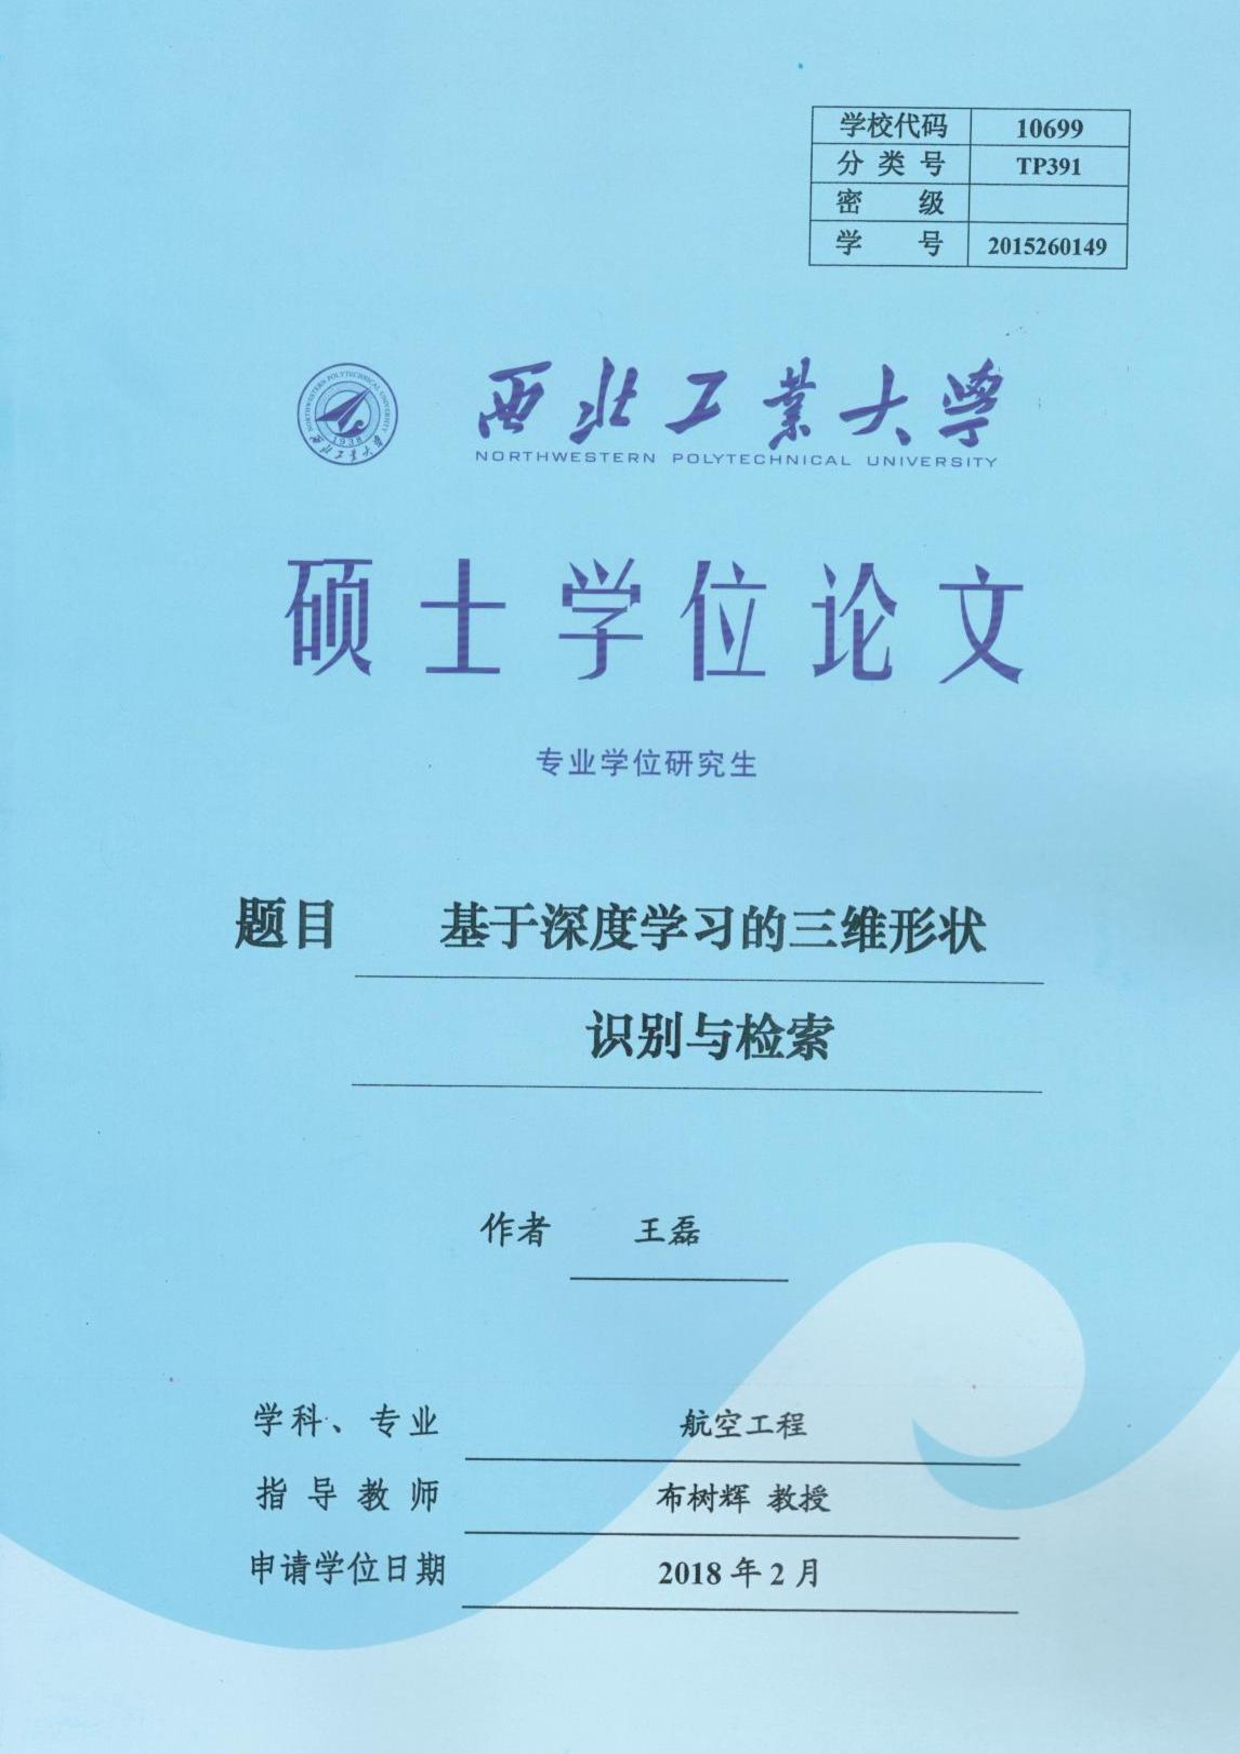
\includepdf{figures/封面.pdf} 
\newpage

\makecover  % 中英文封面
\frontmatter

% 中文摘要
\begin{abstract}

当今人工智能的发展取得了前所未有的成就,无人汽车、虚拟现实、家政机器人等越来越方便人们的生活。由于三维形状物体是人们与外界环境交互的桥梁,因此对三维形状的研究也成为了人工智能研究的方向之一。

如何准确、高效的识别三维形状,其关键就是提取表达能力强、易于区分的三维形状特征。其中,如何设计有效的模型来提取特征是重中之重。三维形状含有比二维图像丰富的信息,例如视觉信息,几何拓扑信息,深度信息等等。在本文中,我们提出了融合视觉信息和几何信息的三维特征学习框架,它有效地结合了不同的模态数据,并通过深度学习来进一步提高单一特征的辨别能力。其中,卷积神经网络(CNN)作用于三维形状的视觉信息,卷积深度置信网络(CDBN)提取了三维形状的几何信息,然后利用两个独立的Deep Belief Networks(DBN)分别从视觉和几何特征中学习高层特征。最后,使用受限玻尔兹曼机(RBM)融合不同模态特征。该融合特征同时表达了三维形状的视觉信息和几何信息,因此具有很强的三维形状表达能力。

%对于3D形状分析来说,一个有效和高效的特征是3D领域推广其应用的关键,其中主要挑战在于设计有效的高级特征。三维形状包含各种有用的信息,其中包括视觉信息,几何关系和其他类型属性。因此提取这些特征的策略是提取有效的三维形态特征的核心。在本文中,我们提出了一种新的三维特征学习框架,它有效地结合了不同的模态数据,通过深度学习来提高单一特征的辨别能力。利用卷积神经网络(CNN)和卷积深信息网络(CDBN)分别提取几何信息和视觉信息,然后利用两个独立的Deep Belief Networks(DBN)从几何和视觉特征中学习高层特征。最后,受限玻尔兹曼机(RBM)训练用于挖掘不同模态之间的深度特征相关性。

于此同时,针对自主机器人的识别要求,探索了利用残缺信息进行三维形状识别,以往的提出的三维形状描述符,具有很强的学习高层次特征的能力,但其中大部分只是使用深度学习方法来提取高层特征,要求数据完备可用。而对于自主机器人而言,获取的信息大多数不具有完备性,因此,本文在对人类识别三维形状的机理的思考上,提出了同时结合深度视觉特征和各个特征之间的时空间关系的模型,来进行三维形状识别。具体而言,使用CNN作为“视觉系统”,利用其具有强大的提取视觉特征的能力,得到高效的视觉特征,然后,利用LSTM这个“记忆系统”学习视觉特征的时空顺序关系,从而得到三维形状特征。该特征综合考虑了从不同视角得到的三维视觉信息的相互关系,因此得到了较好效果。


%同时,在过去的十几年中,一些工作创造性地提出了一些基于深度学习的三维形状描述符,它们具有很强的学习高层次特征的能力,但其中大部分只是使用深度学习方法来提取高层特征,要求数据完备可用。对于自主机器人等实际应用而言,它们不断地从物体上捕捉图像,因此只是利用有限的信息逐步执行物体识别。为了使三维形状识别与检索系统适合移动机器人与环境进行自主交互,需要使用模仿人类的空间相关图像来实现高精度的物体识别。在本文中,我们提出了一种新的三维形状识别和检索框架,它通过记忆机制同时学习高级特征和模型时空信息。具体而言,CNN是“视觉系统”,因为它具有很强的提取有效视觉特征的能力,而LSTM是“记忆系统”,用于学习视觉特征的时空顺序关系。

    \begin{keywords}
        3D形状, 识别, 检索, CNNs, LSTM, 深度学习, 多模态
    \end{keywords}
\end{abstract}

% 英文摘要
\begin{Abstract}

The development of artificial intelligence today has made unprecedented achievements. Unmanned vehicles, virtual reality, domestic robots and other more and more convenient for people's lives. As three-dimensional shape object is a bridge between people and the external environment, the study of three-dimensional shape has also become one of the directions of artificial intelligence research.

How to accurately and efficiently identify three-dimensional shape, the key is to extract the expression ability, easy to distinguish the three-dimensional shape features. Among them, how to design an effective model to extract features is the most important. Three-dimensional shapes contain more information than two-dimensional images, such as visual information, geometric topology information, depth information and so on. In this paper, we propose a three-dimensional feature learning framework that incorporates visual and geometric information that effectively combines different modal data and further enhances the discriminating power of a single feature through deep learning. Among them, the convolutional neural network (CNN) acts on the visual information of the three-dimensional shape. The convolution depth belief network (CDBN) extracts the geometric information of the three-dimensional shape and then uses two independent Deep Belief Networks (DBN) Features learning high-level features. Finally, a Restricted Boltzmann Machines (RBM) is used to fuse different modal features. The fusion feature expresses the visual information and geometric information of the three-dimensional shape at the same time, and therefore has strong ability of three-dimensional shape expression.


At the same time, in view of the requirements of autonomous robots, we explored the use of incomplete information for three-dimensional shape recognition, the previous proposed three-dimensional shape descriptors, has a strong ability to learn high-level features, but most of them just use the depth learning method to extract high-level features, requiring complete data available. For autonomous robots, most of the acquired information is not complete. Therefore, in this paper, we consider the mechanism of human recognition of three-dimensional shape and put forward a model that combines both the deep visual features and the temporal-spatial relationships between the features. For three-dimensional shape recognition. In particular, using CNN as a ``visual system", utilizing its powerful ability of extracting visual features to obtain highly efficient visual features, and then using the ``memory system" of LSTM to learn the spatial-temporal relationship of visual features to obtain a three-dimensional shape feature. This feature takes into account the relationship between the three-dimensional visual information obtained from different perspectives and thus has a good effect.

%For 3D shape analysis, an effective and efficient feature is the key to popularize its applications in 3D domain where the major challenge lies in designing an effective high-level feature. The three-dimensional shape contains various useful information including visual information, geometric relationships, and other type properties. Thus the strategy of exploring these characteristics is the core of extracting effective 3D shape features. In this paper, we propose a novel 3D feature learning framework which combines different modality data effectively to promote the discriminability of uni-modal feature by using deep learning. The geometric information and visual information are extracted by Convolutional Neural Networks (CNNs) and Convolutional Deep Belief Networks (CDBNs), respectively, and then two independent Deep Belief Networks (DBNs) are employed to learn high-level features from geometric and visual features. Finally, a Restricted Boltzmann Machine (RBM) is trained for mining the deep correlations between different modalities. 

%In the past decade, some works creatively proposed kinds of 3D shape descriptors based on deep learning, which have the great ability to learn high-level features.However, most of them just use deep learning methods to extract high-level features, and they require the data completely available.For practical applications such as autonomous robots, they continuously capture images from objects and consequently the object recognition is performed incrementally just using limited information. In order to make the 3D shape recognition and retrieval system suitable for mobile robot to perform autonomous interacting with environment, it is necessary to achieve high accuracy object recognition using spatial-related images which imitates human beings. In this paper, we propose a novel 3D shape recognition and retrieval framework, which learns  high-level features and models spatial-temporal information through memory mechanism simultaneously. In detail, CNNs is `visual system' because it has a strong ability to extract the effective visual feature, while LSTM is `memory system' to learn the spatio-temporal sequential relationship of visual features.
    \begin{Keywords}
        3D Shape,  Recognition, Retrieval,  CNNs,  LSTM, Deep Learning, Multi Modality
    \end{Keywords}
\end{Abstract}



% 目录
\tableofcontents 

\mainmatter  % 

% 第一章
\chapter{绪论}
\section{研究背景及意义}
人类处在一个三维的世界环境中,我们所认识的事物无一不是一个三维的构成的现实物体。人类开展的各种科学研究,都是针对人类所面临的各种科学问题,各种现实问题。这些科学研究有的关于现实世界的感知,有的关于现实物体识别与构建。目前各种智能设备风起云涌,3D场景构建更是炙手可热。这些设备可以对三维场景进行感知,并且模拟出真实的3D场景,从而帮助人们能够在此基础上进行更加高级的运用。例如,虚拟现实技术,无人机、机器人的自主导航技术等等。自动驾驶汽车就是该领域的突出代表,如图\ref{fig_1-1}所示。自动驾驶技术突破了场景识别、场景解析、三维物体识别、三维地图构建、地图构建与定位技术(SLAM)等。

\begin{figure*}[tb]
\begin{center}
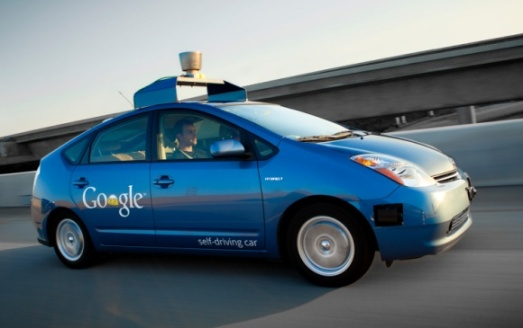
\includegraphics[width=0.4\linewidth, height=5cm]{figures/1-1a.jpg} 
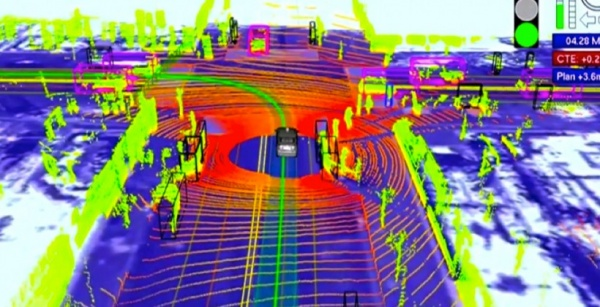
\includegraphics[width=0.4\linewidth, height=5cm]{figures/1-1b.jpg}
\end{center} 
\vspace{-4mm}
\caption{Google自动驾驶汽车和其场景感知的示意} \label{fig_1-1}
\end{figure*}

\begin{figure}[tb]
\begin{center}
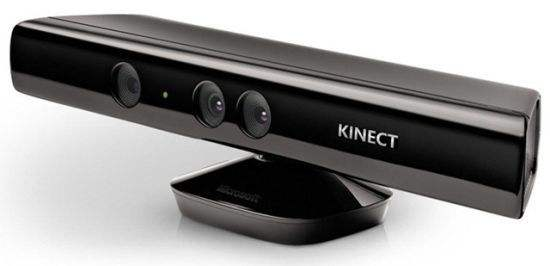
\includegraphics[width=0.4\linewidth]{figures/1-2.jpg} 
\end{center} 
\vspace{-4mm}
\caption{微软发布的首款RGB-D设备Kinect} \label{fig_1-2}
\end{figure}

近年来,业界对三维模型的研究是如火如荼,
%三维模型因为其丰富的形状、颜色、纹理等信息,在多媒体,图形学,虚拟现实,设计,娱乐,工业制造等领域得到了越来越广泛的应用
在工业设计、图形学、虚拟现实等方面被广泛应用\cite{Tangelder2008A}。三维数据库已经硕果累累。同时3D打印技术的出现,使得三维形状模型的应用更加实用化,这种增材制造技术能够完成许多传统减材制造技术所不能完成的复杂产品生产。除此之外,谷歌的Kinect等性价比高的RGB-D设备如图\ref{fig_1-2},更加丰富了三维模型的来源。为了在三维形状的匹配,查找和分类等方面获得优秀的表现,我们需要高效准确的图形检索、分类的方法来处理这些海量三维数据。

三维形状模型与一般的二维图像相比,更丰富真实、更好的符合了人类视觉特性、能够更加清楚的表示现实世界的物体。一般情况下三维形状模型由网格数据结构,包括顶点、面、边等基本数据来表述,因此具有相对复杂的数据结构,与声音、图像相比更加难以处理。三维模型在三维扫描技术与设备以及交互建模技术的发展下迅速增加,方便了研究者的就一步的探索。但由于三维模型较其他类型的数据结构相比复杂,目前仍然存在一些难以解决的问题:前期的三维形状建模工作已经非常成熟,免去了研究者亲自建模的烦恼,可是迅速的识别与检索技术仍然有待解决。另外三维形状匹配还可以在以下领域得到广泛的应用,机器人或无人飞行器通过三维形状匹配在数据库中快速地检索并识别物体,用来寻找并确定目标或者用来躲避障碍物,提高其自身的智能程度;公共安全等领域利用三维匹配技术来查询二维或三维人脸库、三维头颅库等匹配相关信息,能够大大降低恐怖袭击和刑事犯罪对社会的危害;工业现场可以根据图像或图形匹配自动判定控制信息、故障类型等;在生物医学方面,由CT、MRI、PET等断层成像设备产生了大量的三维数据,如何准确快速地查找并处理这些信息,对于提高诊断的准确率并提高我国医疗健康水平,缓解人口老龄化带来的压力至关重要。

传统的三维形状分析技术就是设计出优秀的三维形状特征,这些三维形状特征来自颜色、纹理、形状等不同的属性,能够有效的应对三维形状的分类任务。目前大量用于描述三维模型的特征被提出,例如:平均测地线距离 (Average Geodesic Distance),Si-HKS (Scale-invariant Heat Kernel Signature),SDF (Shape Diameter Function)等,这些特征虽然有一定的效果,但是同时具有一定的局限性。局限一:传统方法的特征要求设计人员具有较强的专业知识和优秀的数学功底;局限二:传统方法的特征针对性很强,即特征只针对某个属性,三维形状的其他信息在提取过程中丢失严重,影响了识别效果。


同时三维形状内容的匹配与检索没有像文本内容匹配与检索那样简单,因为从一篇文章中提取若干关键文字信息,或从一幅图像、一段视频中提取能够代表该图像的描述信息,三维形状的数据结构存在拓扑等复杂结构,因此处理相对复杂,已研究出的特征提取、匹配与检索方法仍存在一定的局限性,因此目前只有具有高级思维的人类才可以完全实现。通过计算机提取多媒体信息的特征仍然是一件困难的事情,也是多媒体匹配与检索的核心技术之一\cite{Tangelder2008A, Funkhouser2005Shape}。三维模型匹配、对齐、分割中,形状特征的提取是非常关键的技术之一,提取的形状特征需要有如下特点:1)良好的类间可分性和类内相似性,用以保证形状描述的准确性;2)对形状变形不敏感,尤其非刚性变形; 3)尽可能低的特征维数,和能够表示三维形状的显著特征,这样就能减少搜索或者匹配的计算量,大大提高计算性能。


%%%%%%%%
%%  \upcite{} 可以使引用变为上标
%%

\section{三维模型的研究状况}

\subsection{国外现状分析}
国外对三维形状识别研究起步较早,研究者主要关注于整体特征的提取,已经获得了大量的研究成果\cite{Tangelder2008A,Funkhouser2005Shape,Krizhevsky2017ImageNet,Kaick2010A,Ullman1985Three, Loncaric1998A, Campbell2001A}。美国Carnegie Mellon大学的Johnson等人\cite{Johnson2002Using}提出了一种经典的局部描述符 Spin Image,该描述符将临近的顶点投影到了一个二维的柱面坐标下,因此复杂的三维形状匹配转化成了相对简单的二维图像的匹配。该方法具有很强的鲁棒性,但这个方法中需要计算并匹配每个顶点的spin image,因此计算效率不高,此外该特征描述符无法很好的应对非刚性变形。之后美国Sarnoff公司的Shan等人\cite{Shan2006Shapeme}提出了使用Shapeme投影的方法来分割需要匹配的形状,从而加速形状匹配的速度; Liu等人\cite{Liu2006Shape}提出了使用Monte Carlo稀疏采样的方法来降低计算量,并使用k-means方法使得到的数据量得到有效的降低从而提高匹配速度。另外希腊Centre for Research and Technology Hellas的Malassiotis等人\cite{Malassiotis2007Snapshots}提出了Snapshot局部特征描述符,该描述符能够很好应对自身的重叠以及假象的影响,并且该方法使用更高效的特征对齐方法,能够获得很好的性能,但仍然无法很好的应对非刚性变形。

大多数情况下,对象物体不仅仅含有刚性变形,还具有非刚性变形,例如弯曲、姿势改变、局部形状变化等。这种变形过程中任意两点测点距离不变,即称之为等距变形。研究者着眼于非刚性形变也做出了巨大贡献。美国ioIMAGE公司的Elad等人\cite{Elad2001Bending}首先在这方面做了尝试,他们根据形状弯曲变形中表面上的长度并未发生变化这一特点,利用MDS(Multidimensional Scaling)完成了测地线距离与欧式距离的转换,相当于复杂的非刚性变形的转化成了简单的刚性形状。之后美国Stanford大学的Emoli等人\cite{M2005A}与以色列的Israel Institute of Technology大学的Bronstein等人\cite{Bronstein2006Efficient}扩展了这项研究,他们使用Gromov-Hausdorff距离来计算形状的相似程度,这样能够有效的降低两个形状建立对应关系时所产生的误差。由于这类方法基于高计算复杂度的最优化方法,因此只能适用于一对一,或者一对少数形状的匹配。德国University of Hannover的Reuter等人\cite{Reuter2006Laplace}尝试使用Laplace-Beltrami谱作为等距变形的形状描述符,这个描述符具有更小的计算复杂度,因此最近受到很大的关注。Wu等人\cite{Wu2010Global}扩展了这个方法,在他们的研究中使用随机采点的方法得到一定数量的顶点,在每个顶点附近选择一个局部区域,选择方法是使用固定面积比率的方式,然后计算该局部区域的Laplace-Beltrami谱,然后与全局的Laplace-Beltrami谱进行结合,这样兼顾了全局和局部特征,因此获得了更好的性能。美国Stanford大学的Sun等人\cite{Sun2009A}提出了HKS(Heat Kernel Signature: HKS)的描述符,通过求解每个顶点的热扩散方程,求取基础解-热核作为局部特征。其优点在于选择不同的扩散时间可以控制所包含的局部范围。该方法只需要特征分解拉普拉斯系数矩阵,效率较高,弱点在于不能应对尺度变换和拉伸变换。以色列的Israel Institute of Technology大学的Bronstein等人\cite{Bronstein2010Scale}改进了热核特征描述符,使之能够应对形状的尺寸变形的影响。

另外一方面,由于三维形状的各个部分的重要程度不同,因此利用区域的重要程度来选择需要匹配的顶点或区域能够极大地降低计算复杂度并提供形状对应、匹配、与检索的速度。首先是美国Maryland大学的Lee等人\cite{Lee2005Mesh}提出了对高斯加权平均曲率做center-surround的网格显著区域提取的方法,通过实验得知该方法能够捕获网格上绝大多数的显著区域,但该方法的缺陷是得到的显著区域过于稀疏,导致形状匹配精度的下降。之后,美国Princeton大学的Shilane等人\cite{Shilane2007Distinctive}提出另一种形状显著区域提取的方法,任意一个给定顶点对已建立的数据库进行检索,使用DCG(discounted cumulative gain)值来进行该点附近的显著区域检测,若使用该区域检索能够获得高的DCG值,则表明该区域是重要,反之则认为是普通的区域相对不重要。该方法能够提供更高精度的局部显著指标,然而这个方法由于计算量大,并且需要事先构建一个形状数据库,因此比较难以在实际中应用。波兰Institute of Theoretical and Applied informatics of PAS的Glomb\cite{G2009Detection}将图像领域的Harris运算符扩展到了三维领域,通过计算顶点附近区域的形状变化来衡量该点局部区域的显著程度。法国INRIA Grenoble Rhone-Alpes的Zaharescu等人\cite{Zaharescu2009Surface}将图像领域内知名的DOG(Difference of Gaussians)方法在三维形状方面进行了尝试,并提出了Mesh DOG方法,该方法具有对方向、旋转、平移和缩放具有较高的鲁棒性,但仍然不能很好的应对非刚性变形。

由于三维形状的匹配与检索相对复杂,很难推导出理论的评价方程,因此常常使用标准形状库来评价各种方法。美国Princeton大学的Shilane等人\cite{Shilane2004The}提出一套三维模型库Princeton Shape Benchmark,该数据库包含了1814个通用物体模型,并分成了训练和测试两组。加拿大McGill大学Siddiqi等人\cite{Siddiqi2008Retrieving}提出了专门针对关节变形物体的形状标准库McGill 3D Shape Benchmark。以色列Israel Institute of Technology大学的Bronstein等人\cite{Bronstein2009Numerical}设计并制作了专门针对非刚性变形的形状标准库TOSCA,可供部分匹配和检索研究之用。美国国家标准与技术研究院提出的SHREC2011非刚性变形形状库\cite{Lian2011SHREC},包含600个非刚性变形的物体,适合包含非刚性变形方面的分析与评价

\subsection{国内现状分析}

国内在三维形状特征描述符方面起步较晚,研究主要集中在全局特征描述符上,经过近几年的努力取得了可喜的研究成果。刘等人\cite{刘志2016基于特征线条的三维模型检索方法}为了避免在三维模型检索中对输入源的限制,提出一种以自然图像为输入源、基于特征线条的三维模型检索方法。黄等人\cite{黄骥2016基于核线性分类分析的三维模型检索算法}为提高检索精确度,提出了一种利用核线性分类分析来对模型特征进行优化的新方法。张等人\cite{张全贵2017融合}针对手绘草图检索三维模型时存在的表达模糊性和绘制随意性等问题,提出基于Fuzzy拓扑关系与角点典型形状上下文(CRSC)的三维模型检索方法。李等人\cite{李闯2016基于平均自旋图的三维形状特征描述}基于自旋坐标和自旋图理论,给出基于平均自旋图的三维形状特征描述方法,用于三维模型检索。周等人\cite{周燕2016基于多特征融合的三维模型检索算法}针对三维模型检索中单一特征检索效果差的难题,首先提出了三维模型的3类特征向量提取算法,即刻画模型表面特性的扩展高斯球面特征向量、反映模型内部结构的Radon变换球面分布特征向量、代表模型投影层次的视图分层压缩感知特征向量。其次,以样本模型的查询结果分类信息熵作为指标并结合监督学习过程,给出了一种多特征融合的加权系数估算方法。

\section{深度学习技术}

深度学习(Deep Learning)由于其出色的表现,逐渐使得其成为研究的热点。针对深层次网络训练的难题,人们提出了BP算法\cite{Rumelhart1988Learning}。BP算法是深度学习的基础算法之一。Yann LeCun等\cite{Lecun2014Backpropagation}提出了卷积神经网络(Convolutional Neural Network)使人们看到深度学习的巨大潜力。然而,能够训练的网络深度只有两到三层,严重抑制了深度学习的发展进步。事情的转机出现在2006年,由于深度置信网络模型(DBN)的巨大突破,使得深度学习开始产生。Hinton等人\cite{Hinton2006A}使用贪婪算法对网络参数进行自底向上进行逐层预训练,由此可对前馈网络模型进行预训练。
%
随着深度学习技术不断发展,大量的新的深度学习算法被提出。其中比较出色的包括自动编码器(AutoEncoder)、卷积神经网络(CNN)、循环神经网络(RNN)、深度神经网络(DNN)、深度玻尔兹曼机(DBM)、卷积深度置信网络(CDBN)等等。2012年,Alex等人利用卷积神经网络设计的算法在Imagenet图像识别竞赛中表现优秀\cite{Krizhevsky2017ImageNet},在后续图像各方面的研究中,这种类型的卷积神经网络都已经被广泛采用。而在声音识别领域,百度公司采用深度学习方法研发出的语音识别系统Deep Speech,也能取得非常好的识别效果\cite{Niu2014Context}。

近年随着深度学习算法的深入研究,深度学习算法已经深入到IT领域的各个方面,各个互联网巨头都不惜重金,发展深度学习,例如腾讯的DX-I框架,阿里巴巴的PAI2.0框架。Google的Deepmind团队的AlphaGo更是在围棋方面战胜世界一流棋手李世石。不久前更是推出了``最强版”AlphaGo Zero。深度学习已经是目前的风口浪尖,其能够通过学习的方式得到表达能力更强的阶层式特征,并对海量数据进行处理,因此深度学习的方法可以应用于三维形状的识别问题。一般的特征包括颜色的直方图,纹理的直方图,Gist,HoG, SIFT, SURF等,尽管这些特征在某些应用中取得了比较理想的效果,但是它们只能刻画图像当中某一方面的信息,也就是说这些特征在不同的任务中,效果并不都是最优的。
%
最近几年越来越多的研究表明,特征的提取和分类是相互交织在一起的,通过学习方式得到的特征能够获得更高的性能。图像信息在人类理解和认知外界环境中起到主要的作用,将图像信号经过人脑视觉系统处理之后,我们能够对物体进行识别、对场景进行理解,从而使得我们能够对环境做出反应。但是,为什么人脑有如此强大的信息处理能力,从而让我们在短时间之内对环境做出非常准确的理解与判断?以及怎样才能让机器模拟人的大脑视觉系统处理图像?神经生物学家、生物医学家对人脑进行研究发现大脑的视觉系统处理是一种“分层学习” 机制,如图\ref{fig_brain}所示。

\begin{figure}[tb]
\begin{center}
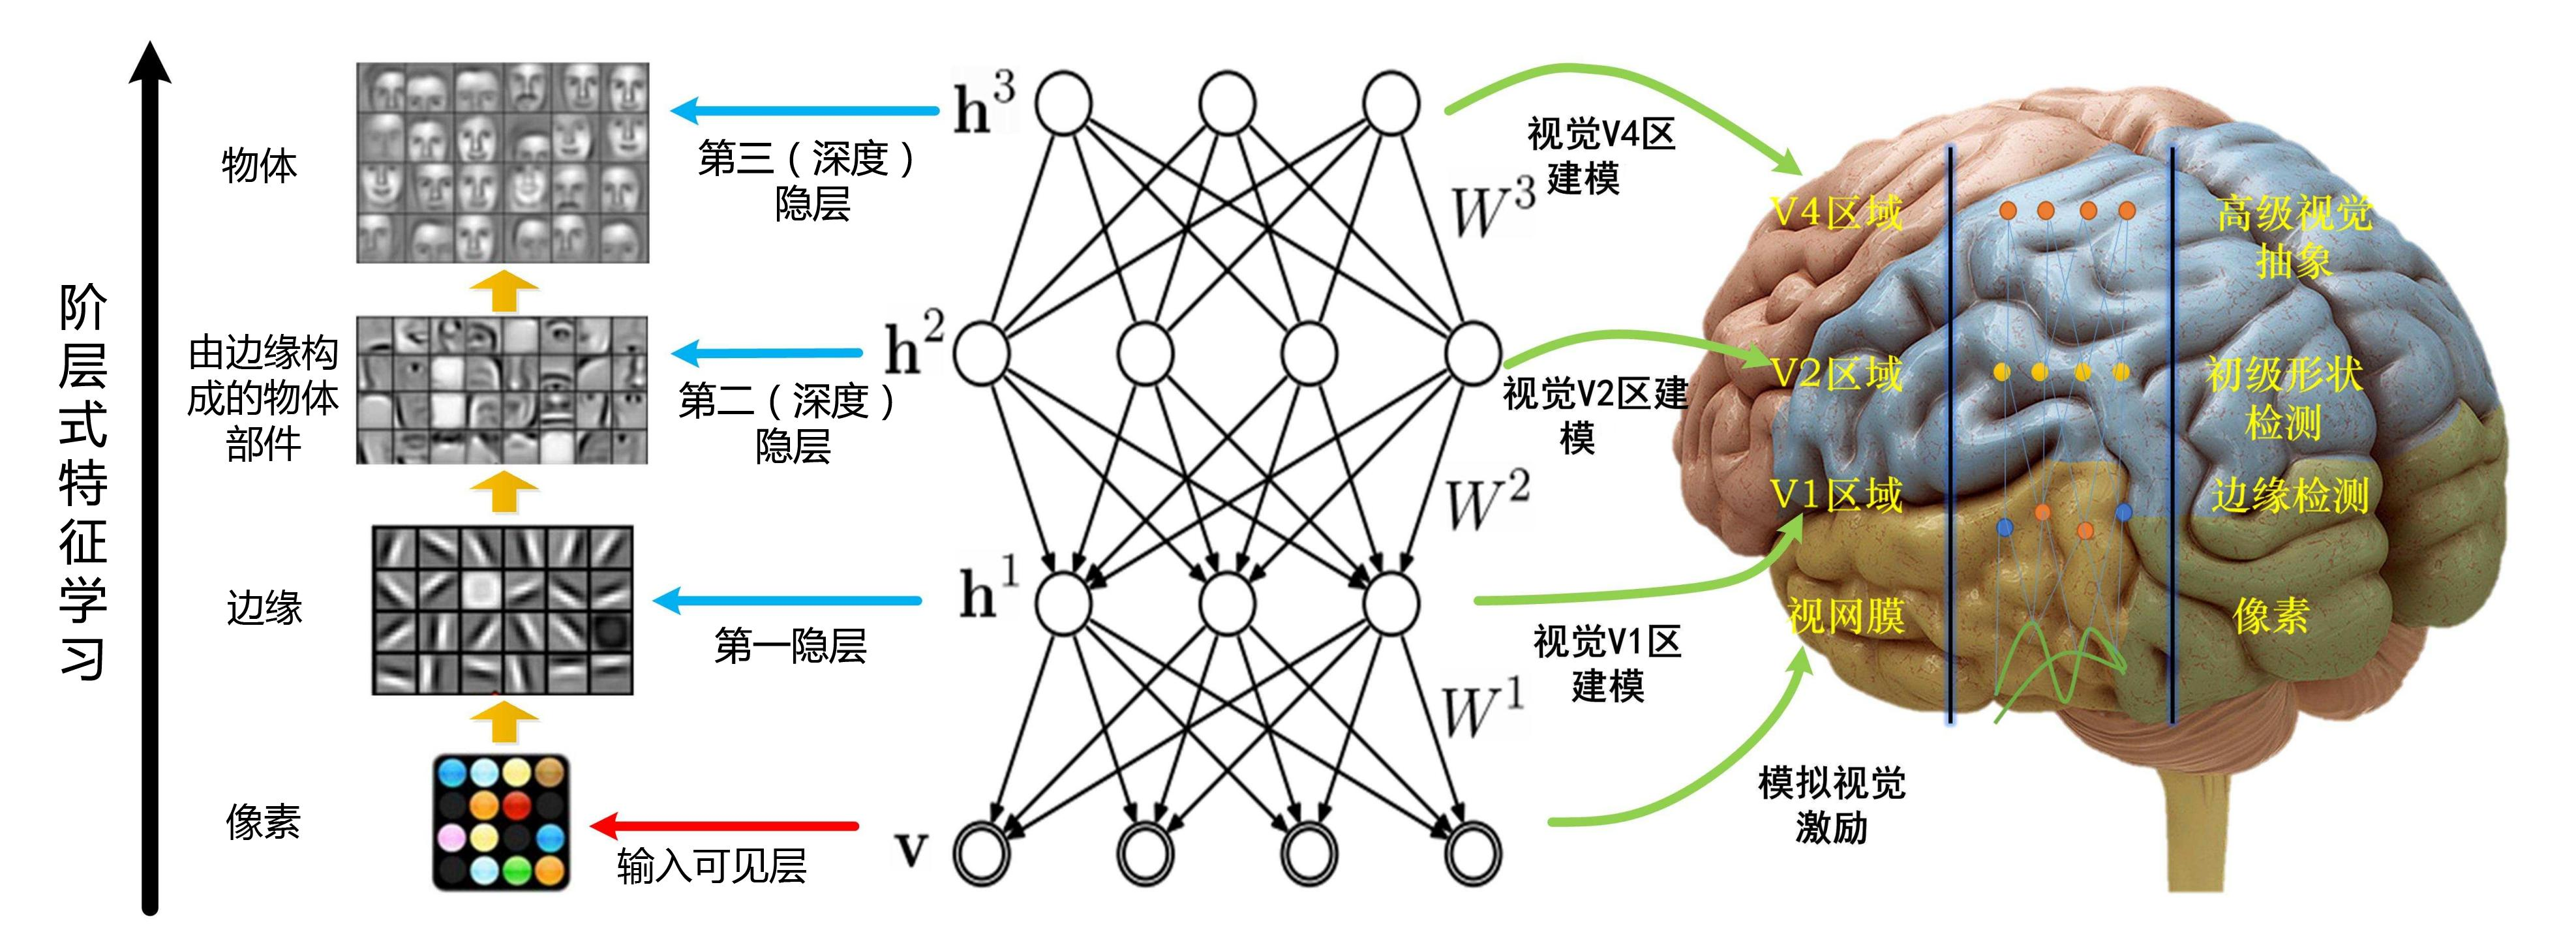
\includegraphics[width=0.9\linewidth]{figures/1-3.jpg} 
\end{center} 
\vspace{-4mm}
\caption{大脑认知和深度学习的关系(示意图)} \label{fig_brain}
\end{figure}

从原始信号摄入开始,接着做初步的处理,然后抽象,然后进一步分析。人类的这种分级认知机制,从机器处理图像的角度来看是一种从低级特征提取到高层特征提取的过程。因此,实现机器像人类一样认知三维形状,图像的特征提取至关重要。如果想要模拟人类视觉系统的分层学习机制,则需要经验丰富的算法设计工程师根据不同的需求,设计出不同层次的特征提取方法,工作量很大并且缺少通用能力。

另一方面,在机器学习领域,目前常用的学习算法例如支持向量机、提升算法,普通的神经网络等都是浅层模型,这些方法的模型通常只有1-3个信息处理层,无法处理现实世界的高度复杂的非线性数据;而人类的大脑的认识、学习是通过多层次的处理来实现的,从而使解决问题的规模可以非常庞大。最近十年间,由于新的神经网络学习方法的研究和计算机能力的提高,克服了以往神经网络层数多而导致的无法训练、过拟合等问题,从而使深度学习得到了快速的发展。最新的研究成果表明,通过深度学习,能够让计算机生成较高层次的语义信息,因此能够填补底层特征和高层语义之间的鸿沟,所以能够极大地提升人工智能的程度。

深度学习已广泛应用于自然语言处理,语音识别,计算机视觉等诸多领域,并展示出了非常优异的性能\cite{Krizhevsky2017ImageNet, He2015Delving, Mnih2015Human}。Dahl等人\cite{Dahl2012Context}提出了一种融合隐马尔科夫模型的混合深度网络,并且在语音识别方面获得巨大成功,在非常具有挑战的数据库上获得了理想的识别精度。Lee等人\cite{Honglak2009Convolutional}使用了卷积深度置信网络来提取图像的阶层特征,在几个图像数据库上都获得较好的识别率。Nitish等人\cite{Srivastava2012Multimodal}提出了多模态的深度学习方法,他们使用了两个深度置信网络来对图像数据和文本标签数据进行建模,并在两个深度网络的上层构建了一个联合表达层来表达这两种数据的关联性。与传统的支持向量机方法相比,该方法能够充分利用多种来源的信息,因此能够获得更高的性能。Kae等人\cite{Kae2013Augmenting}提出了一种融合CRF和玻尔兹曼机的图像标签方法,通过这种融合使深度学习方法提高了结构学习能力。

\section{论文的研究内容及贡献}
目前深度学习(Deep Learning, DL)已经广泛应用于各个领域,可是在三维形状领域目前还不成熟。对三维形状识别检索领域的不断探索,能够不断拓宽深度学习在三维形状分析领域的应用,不断提高三维形状的识别精度,使其更好的服务于社会生产中去。具体来说,论文的贡献如下:

\begin{itemize}
\item 结合多模态融合的思想,首次提出了结合CNN、CDBN、DBN、RBM的多层神经网络的多模态信息融合方法,从而得到具有强表达性质的三维形状特征。
\item 提出了利用获取三维形状视觉信息具有序列化时空信息,提出了基于CNN、LSTM的三维形状识别方法
\end{itemize} 

\section{论文结构安排}

第一章绪论部分介绍了本文的研究背景及意义,说明了本文的研究内容和主要贡献。

第二章详细分析了目前深度学习技术在三维形状应用的最新进展。

第三章详细介绍结合CNN、CDBN、DBN、RBM的多层神经网络的多模态信息融合方法。

第四章详细介绍了基于CNN、LSTM的三维形状识别方法。

第五章对本文工作做了总结,并对后续工作进行了展望。


% 第二章

\chapter{深度学习在三维形状分析领域的进展}

随着深度学习的不断发展,不仅在计算机视觉方向取得了巨大成功,而且也被广泛应用于三维形状领域,并且取得了一定的成绩。由于三维形状复杂的拓扑结构和丰富的几何信息,如何将深度学习成功的应用于三维形状领域是一大挑战。为了解决三维形状的识别和检索任务,研究人员们主要沿着如下五个不同的方向进行研究。

\begin{enumerate}
\item 从三维形状中提取描述特征,将其作为深度神经网络的输入,进行学习。
\item 使用目前流行低成本RGB-D相机(Kinect)捕获RGB-D信息,将其作为深度神经网络输入。
\item 直接作用于3D数据的深度神经网络,学习3D形状特征。
\item 利用从不同角度观察三维形状得到的二维图,将三维问题转化为二维问题,之后再利用深度学习方法得到高效的、鲁棒性强的三维形状特征。
\item 深度神经网络作用于超光谱相机拍摄的3D数据。
\end{enumerate}

\section{DL作用于三维模型低层特征}

三维模型低层特征描述符常常被用来进行3D数据的识别检索任务。然而,在三维领域中,由于三维数据的复杂性,通常需要高效率的三维形状描述符。通常的做法是提取的低级别的描述符,之后将他们作为深度神经网络(DNN)的输入,从而使识别和检索任务能有高层次的表现。
\begin{figure}[tb]
\begin{center}
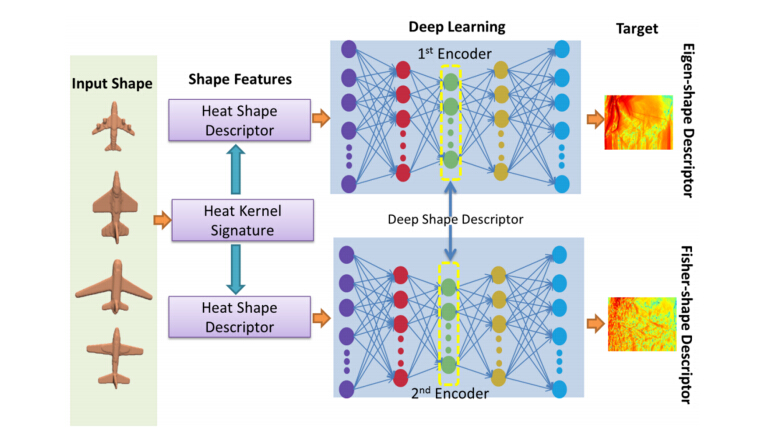
\includegraphics[width=0.9\linewidth]{figures/Fang.jpg} 
\end{center} 
\vspace{-4mm}
\caption{Fang等人提出的三维深度形状特征描述子} 
\label{fig_Fang}
\end{figure}

Liu等人\cite{Liu2014High}采用了深度置信网络(DBN)进行学习3D数据的训练学习,他们采用来自3D数据的底层特征作为DBN的输入数据。具体来说,首先获取每个3D形状的200张深度图像,然后提取每张深度图的SIFT特征描述子。之后,构建BOW字包模型,其中SIFT描述子被编码成BOW模型的``单词''。这些来自三维模型的BOW特征向量,作为DBN的输入数据,对DBN进行逐层的贪婪算法的训练,得到高表达能力的3D特征描述子。该实验同时进行了3D形状的分类和检索实验。实验结果表明该方法获得了比标准BOW模型更为优秀的表现效果,同时证明了在3D数据分析领域深度学习技术具有优秀的效果,并能产生高水平的特征描述子。Bu等人\cite{Bu2014Learning}所作的工作是结合Scale Invariant Heat Kernel Signature (SI-HKS) 和 Average Geodesic Distance (AGD)这两种来自3D数据的局部特征描述子,组成一个低层的3D特征,该特征是由SI-HKS的前6个频率分量和AGD值组成的。接着,一个被称做Geodesics-Aware Bag-of-Features (GA-BoF)的BOW模型的变种被生成。接下来,从GA-BOF中获得的中层特征描述子被用来训练DBN模型,其中DBN的训练采用对比散度的方法。从DBN出来便得到了高层特征描述子。对于3D数据的分类实验中,DBN被认为是一种降维方法,因此他们比较了类似的降维方法,像Principal Component Analysis (PCA) 和 Multi-Dimensional Scaling (MDS)。对于3D模型的检索实验中,DBN模型对比了一些常见的3D数据特征描述子,像Heat Kernel Signature (HKS)。实验结果表明高层特征描述子相较于常见的特征描述子具有更好的可区分性,增强了分类与检索效果。这些被DBN生成的高层特征描述符,又被称做局部深度特征(Local Deep Feature)。在之后的相关工作中,Bu等人利用了基于GPU的深度学习工具包,加快了整个算法的运行速度。

Xie等人\cite{Xie2015Deepshape}将3D形状在不同尺度下的Heat Kernel Signature(HKS)的分布提取出来,用作3D数据的低层特征描述子。这个多尺度的分布特征被用来作为AutoEncoder(AE)深度网络模型的输入,从而获取高层特征描述子。为了提高特征描述子的判别能力,采用了Fisher判别准则。该三维数据的特征表达是由AE的所有激活状态的隐层链接而成。三维形状的匹配和检索实验表明,该高层特征描述子具有鲁棒性对变形不敏感。2015年,Fang等人\cite{Fang20153D}提出了类似的深度学习框架,作者提出的深层三维形状描述符,是利用Heat Shape Descriptor(HeatSD)的方法,该方法是由基于HKS的不同尺度下的形状描述子和多对一的编码器构成。多对一编码器确保了完全相同的输出是由相同类的输入产生。主成分分析(PCA)和线性判别分析(LDA)用于提取三维模型生成特征的形状描述符特征的形状描述符和Fisher的形状描述符(FSD)。预先计算的ESDs和FSDs被作为目标值,分别用来训练两个独立的编码器。该方法同时最大化了类间的边缘和最小化了类内的方差,提高了深度形状特征描述子的判别能力。整个流程图如图\ref{fig_Fang}所示,三维形状特征描述子子在三维形状检索中取得了良好的效果。

\section{DL作用于RGB-D数据}

随着RGB-D传感器逐渐普及,像微软的Kinect传感器,人们可以轻易的获得大量的三维形状的RGB-D数据。这种传感器除了提供常见的RGB三通道的颜色信息外,还提供了额外的深度信息,因此许多研究工作利用这些来自三维模型的RGB-D信息处理诸如3D形状识别、检索和语义分割等信息\cite{Sanchez2016A}。

Socher等人\cite{Socher2012Convolutional}首先提出了基于RGB-D数据对三位形状进行分类的方法。提出了卷积与递归神经网络(RNN)相结合,分别处理颜色信息和深度信息的方法。具体来说,首先,利用两个单层的CNNs分别提取RGB图像和深度图像的低层特征描述子。然后,不同的CNNs的输出被输入到不同的RNN模型中去,其中模型的所有权重都是随即初始化的。从RNN中得到的每一个特征最终被合并成一个特征,同时将其带入到一个联合的softmax分类器中。该方法在对家庭中的三维形状分析中具有精确的性能。Couprie等人\cite{Couprie2013Indoor}采用了多尺度的CNN用来对室内的RGB-D场景进行语义分割。该网络能够处理三个不同尺度的深度图像和RGB图像,然后这些分别得到的上采样结果被合并成一个特征,之后被带入到分类器中从而得到分类标签。最终的分类标签同时融合了分类器的预测结果和RGB-D场景的超像素分割的结果。实验表明,这种方法比在这之前的方法更加有效,运行速度更快。Alexandre\cite{Alexandre20123D}探索了在CNNs之间使用迁移学习用来对3D模型进行识别的可能。该方法应用了四个独立的CNN处理RGB-D图像的四个独立的通道信息。四个CNN依次的进行训练,其中将上一个训练好的CNN权重作为下一个CNN的输入。10个类别的3D物体的实验表明,所提出的训练策略可以提高三维形状分析性能。

在Schwarz等人\cite{Schwarz2015RGB}的基于深度CNN网络的迁移学习也是致力于解决RGB-D物体的识别。其架构采用了一个预训练的CNN进行图像分类,同时将颜色和深度信息分开作为输入对CNN进行训练。同时对输入数据进行必要的预处理从而转换成相应的格式。Schwarz认为深度信息方面,应该从一个规范的视角来渲染物体,同时根据据物体中心不同的距离来对深度进行着色。实验使用网络的最后两个FC层的输出作为描述符,而SVMs最终被用来预测被测试对象的类别、实例和姿态。Eitel等人\cite{Eitel2015Multimodal}也提出了解决RGB-D物体识别的方法。其设计了一个两流CNN结构用来RGB-D物体的识别任务。这两个流(一个用于颜色,另一个用于深度)包含五个卷积和两个FC层。两流原本单独训练,随后,他们在之后的FC层和softmax分类器中被融合。 由于用来完成识别任务的两个CNNs的需要预训练才能完成基于ImageNet数据集的物体识别任务,因此对输入数据进行预处理,尤其是深度信息的处理,是非常必要的。像这种将深度信息编码成彩色图像的方法,被实验证明,效果优于当时其他现存方法。此外,一种新的数据增强方案被采用,该方案生成人工噪声模式,并将它们用作额外的训练样本。大量的实验结果表明,所提出的方法在真实场景、噪声场景中的目标识别任务中具有很好的性能。 Feng等人\cite{Feng20163D}提出了一个集成的CAES(如图\ref{fig_Feng}),利用从类似Kinect的相机获取的一张深度图来解决三维形状的检索问题。每个AE都使用SDG在不同的数据库CAD模型上进行训练。由于该查询不同的数据类型(例如,深度数据)对训练数据的比较(例如CAD模型),所有的AES输出结果转发到一个新的层,称为域适应层(DAL),以确定检索排行。实验结果表明,与其他相关方法相比,该方法获得了更好的性能,比如方向梯度直方图(HOG)描述子,使用L2范数或全局AE。 

\begin{figure*}[htbp]
\begin{center}
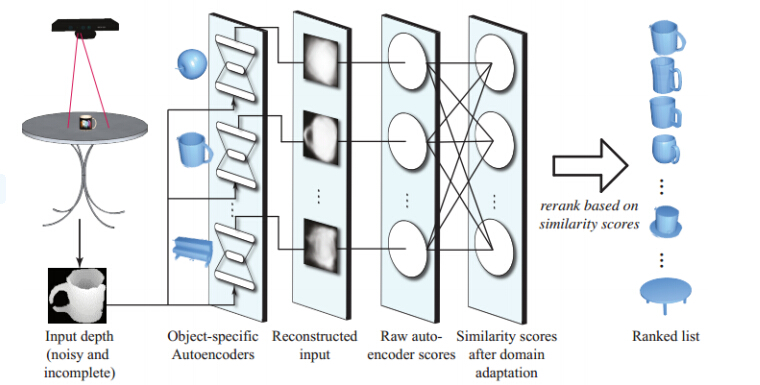
\includegraphics[width=0.9\linewidth]{figures/Feng.jpg} 
\end{center} 
\vspace{-4mm}
\caption{基于深度的压缩自编码器的检索框架} 
\label{fig_Feng}
\end{figure*}

\section{DL作用于3D数据本身}
在过去的几年中,利用捕获场景的完整三维几何图形直接作为DNN的输入的方法已经开始出现。Wu等人\cite{Wu20143D}提出了一种利用整个三维结构实现三维形状表征的新方法。该方法被称为3D ShapeNets,其基本结构为以三维形状作为深度神经网络的输入。这种输入是三维体素网格,这是一种二进制表达,即就是我们认为某个体素网格是否属于该三位形状的一部分。这种体素网格作为之后的DBN的输入,进行训练学习。为了减少与正常分辨率的三维体素量进行全连接时,DBN所需参数数量巨大,于是采用了三维滤波器卷积来降低参数数量。最特别的是,其提出了卷积深度信念网络(CDBN),CDBN一共包含五层,其中三层卷积,一个完全连接层,和一个输出层。该模型首先进行逐层初始化,之后,通过反向传播算法进行微调。标准对比散度被用来训练网络前四层,但更复杂的快速持续对比散度(FPCD)被用于训练网络的顶层。该框架在被用在多种任务,例如三维形状的分类和检索,下一个最好视角预测和基于视图的2.5D的识别任务,在这些任务中都表现优异的效果。此外,作者还发布了ModelNet数据集,这是一个全新的大尺度三维数据集,包括662个不同类型的CAD模型。

Maturana和Scherer\cite{Maturana2015VoxNet}也尝试了使用三维数据的空间表达式进行三维模型的识别方法。如图\ref{fig_Maturana}所示,该VoxNet框架是由体积大小为32×32×32体素网格,该体素网格产生于点云的分割之中,之后将其作为CNN的输入进行训练。该网络架构是由两个带有3D滤波器的卷积,一个池化层和两个全链接(FC)层构成,采用带有动量的随即梯度下降(SGD)的算法进行训练。每一个点云的分割部分,被预测得到一个预测标签。
\begin{figure}[tb]
\begin{center}
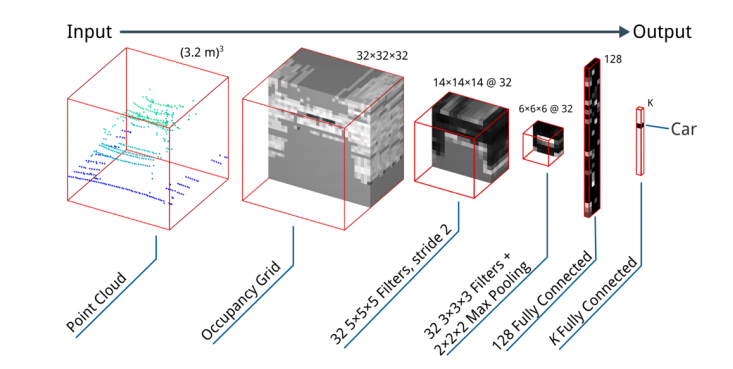
\includegraphics[width=0.9\linewidth]{figures/Maturana.jpg} 
\end{center} 
\vspace{-4mm}
\caption{三维模型的识别的VoxNet4架构} 
\label{fig_Maturana}
\end{figure}
Maturana采用了三个不同领域的三维数据,分别是激光雷达点云数据,RGB-D点云数据和CAD模型,来评价VoxNet模型。实验表明,该框架结构对比同类方法表现更好,同时具有一定的实时性。具体来说,VoxNet的性能表现优于3D ShapeNets\cite{Wu20143D}在三维形状分类的任务中。该实验所采用的数据集是ModelNet10, ModelNet40和NYU v2\cite{Silberman2012Indoor}。另一方面,当使用ModelNet10预训练的模型时,3D ShapeNets在NYU v2数据集上表现更好。 Sedaghat等人\cite{Sedaghat2016Orientation}修改了VoxNet的架构,以便将模型的方向性考虑进去。在最后的模型中,类标签直接从激活的方形中得到。 该方法改进了ModelNet10和其他数据集的分类结果。

Wang等人\cite{Wang2016An}最近提出了一种新的3D描述符学习方法,即卷积自动编码器极限学习机(Convolutional AutoEncoder Extreme Learning Machine, CAE-ELM)。其结合了CNNs, AEs和ELMs的优势。极限学习机(ELM)是Huang等人\cite{Huang2006Extreme}提出的只包含一个隐藏层的前馈网络。ELM的隐含层实际上是固定的和随机的,而输出层是根据感兴趣的任务以监督的方式训练的。Kasun等人\cite{Kasun2013Repre}提出了具有多隐层的标准ELM模型的深入扩展。Wang等人\cite{Wang2016An}提出的架构包括以下几个部分:(i)卷积特征图生成:在这部分网络中,计算三维输入数据(即体素和有符号距离场(SDF)数据)与随机生成的三维内核和卷积特征地图。接下来,为了保持旋转不变性,对特征图应用平均池化。(ii)AE描述符提取:池化之后,每个特征图被作为输入提供给单独的AE。所有的AE最初都是用随机权重初始化的,最后的(输出)权重是通过训练学习的。(iii)ELM分类器:在网络的最后部分,从AE提取的所有描述符被连接成用于预测当前3D形状的标签的矢量。在三维模型分类,三维形状检索和三维形状完成的背景下,CAE-ELM在ModelNet上进行了测试,与Wu等人\cite{Wu20143D}和Xie等人\cite{Xie2015Deepshape}的方法相比,取得了优势。实验中使用的最终体系结构包括两个平行的CAE-ELM层,一个在体素上,另一个在SDF数据上。Han等人\cite{Han2016Mesh}提出了用于从3D网格学习高判别性3D特征的网格卷积限制玻尔兹曼机器(Mesh Convolutional Restricted Boltzmann Machines, MCRBM)。学习得到的特征保留了局部区域之间的结构关系,同时也可以保留局部与全局之间的结构关系。该结构提供了局部区域的新的原始表示,称为局部函数能量分布(Local Function Energy Distribution, LFED),作为对网络的输入。另外,将多个MCRBM组合起来,形成一个更深的模型,命名为网格卷积深度置信网络(Mesh Convolutional Deep Belief Network, MCDBN)。这两种深度模型在进行了全局和局部形状检索和形状对应的情况下,表现了优于诸如BOW,Chen等人\cite{Chen2003On},Kazhdan等人\cite{Kazhdan2003Rotation},Bronstein and Kokkinos等人\cite{Bronstein2010Scale}和Wu等人\cite{Wu20143D}的方法

Qi等人\cite{Qi2016Volumetric}在开创性的工作中,详细阐述了影响体积CNN性能的两个因素,即网络体系结构和体积分辨率,并提出了两种新的CNN体​​系结构,这些体系结构改善了目标分类当前的最新性能,即VoxNet\cite{Maturana2015VoxNet}平均课程准确率达到83%。Lin等人\cite{Lin2013Network}第一个提出的CNN包括的mlpconv层的3D扩展工作,并试图通过包括对对象的部分进行分类的附加学习任务来强调3D物体的细节。这个网络达到了86%的平均分类准确度。第二个CNN最初利用长各向异性核来考虑长距离相互作用,并开发了一个适应性的NIN网络\cite{Lin2013Network}进行分类,平均分类准确率为85.6%。在这两个网络中,还通过应用几个方位角和高程旋转来训练数据增强,同时还使用了多方位池化,从而进一步提高了性能。广泛的实验评估强调了三维分辨率在体积CNN中的重要性。最近,Brock等人\cite{Brock2016Generative}提出了用于形状建模和3D形状分类的基于体素的(全3D)模型,并且与迄今为止提出的任何其他3D或多视图深度学习方法相比,ModelNet10和ModelNet40的大量分类结果得到改善。作者利用了DNN领域的最新进展,并设计了一种网络模型,其依赖于(i)初始式模块的结构\cite{Szegedy2016Inception}(ii)批量标准化\cite{Ioffe2015Batch}(iii)预先激活的剩余联系\cite{He2016Identity}和(iv)随机网络深度\cite{Huang2016Deep}。所提出的模型Voxception-ResNet(VRN)是45层深。作者使用整合VRN模型得到了ModelNet40和ModelNet10的最新分类结果。 应该指出的是,训练如此深的模型需要大量的数据增强。

Song和Xiao\cite{Song2015Deep}提出了一种用于在RGB-D场景中进行3D对象检测和识别的流程,称为Deep Sliding Shapes。有趣的是,Song和Xiao不是使用了深度通道,而是通过使用定向截断有符号距离函数(TSDF)将每个深度图像转换为完整的三维体素网格来利用场景的原始3D信息。然后利用被称为3D区域建议网络(RPN)的完全3D卷积网络,以从两个不同尺度的3D体素网格生成3D对象边界框,以便能够处理不同的对象尺寸。同时还为每个生成的建议对象提议提供了对象分数。此外,每个检测到的3D建议框及其对应的2D色块(即,3D建议框的2D投影)分别被馈送到3D ConvNet和2D ConvNet,以便同时学习物体的类别和3D框回归。对于在三位形状领域的目标评估,该方法优于最先进的选择性搜索方法(Selective Search method)\cite{Uijlings2013Selective},而“深度滑动形状”\cite{Song2015Deep}的目标检测任务与其“非深度”版本相比较,即手工描述符的3D滑动形状\cite{Song2014Sliding}和带有ConvNets描述符的最先进的2D Depth-RCNN\cite{Gupta2014Learning},具有较为优异的性能。


\section{DL作用于3D模型的2D投影/视图}
为了表达3D形状/模型而从不同方向采集的多个2D投影是三维形状分析和理解通常采用的“技巧”。Zhu等人\cite{Zhu2014Deep}通过投影到二维空间来构建3D形状的深度学习的框架,是类似的最早的方法之一。在前面提到的工作中,为了在3D形状检索的应用场景中生成3D形状的全局深度表示,使用了AE。对每个三维模型在位移和尺度方面进行姿态归一化,随后收集他们的一系列二维投影。在用投影预先训练堆叠的RBM之后,使用反向传播对AE进行微调以最小化重建误差。最后,隐藏层用于表示检索过程中3D形状的相应投影/视图。由于每个模型生成不止一个编码(每个投影一个),所以使用Hausdorff距离的变体来计算两个不同3D形状的最终表示之间的距离。实验是在两个流行的数据集进行的,即普林斯顿形状基准(PSB)\cite{Shilane2004The}和工程形状基准(ESB)\cite{Jayanti2006Developing}。结果表明所提出的架构与其他基于全局描述符的方法LFD\cite{Chen2003On}相比表现更好。此外,基于SIFT的BoW这种全局特征与局部特征的线性组合,是性能有所提升。

Leng等人\cite{Leng20153D}利用自编码器实现了三维形状检索的工作。在其工作中,提出了从CNN启发的标准AE的扩展,称为堆叠局部卷积自动编码器(Stacked Local Convolutional AutoEncoder, SLCAE)。局部卷积自动编码器(LCAE)通过使用卷积运算将局部连接的层代替标准AE的FC层而构建。在LCAE的堆叠版本中,许多编码器被放置在彼此的顶部,并且最后一个的输出被用作三维模型的表示。提供给所提出的AE的输入是三维形状的多个视图的多个深度图像,而该架构的每一层都是使用梯度下降法来训练的。堆叠局部卷积自动编码器(SLCAE)与其他优秀的方法在三个三维形状数据集上进行比较,获得了更好的结果。这三个三维形状数据集分别是PSB\cite{Shilane2004The}, 台湾大学数据集(NTU)\cite{Chen2003On}, SHREC'09\cite{Godil2009SHREC}。另外一个叫做3D卷积神经网络(3DCNN)的架构是由Leng等人提出的\cite{Godil2009SHREC}用于同时处理3D对象的多个2D视图。每个形状的视图在被馈送到网络之前被分类成三个合理的序列,以使视图以固定的顺序被列出。3DCNN由四个卷积层,三个子采样层和两个FC层组成。 卷积层最初是以训练AE的相同方式预训练的。之后,整个网络使用反向传播进行了微调。第一个FC层的输出被用作检索的输入数据的表示。对三个数据集(即PSB,NTU,SHREC'09)的评估表明,与其他最先进的方法相比,所提出的方法具有显着的性能。尽管3DCNN表示虽然取得了良好的结果,但是与使用SLCAE\cite{Leng20153D}获得的检索性能相比,在所所使用的3个数据集中其性能性能偏低,这表明后者的表示可能是一个更好的选择来处理三维形状的检索工作。
\begin{figure}[tb]
\begin{center}
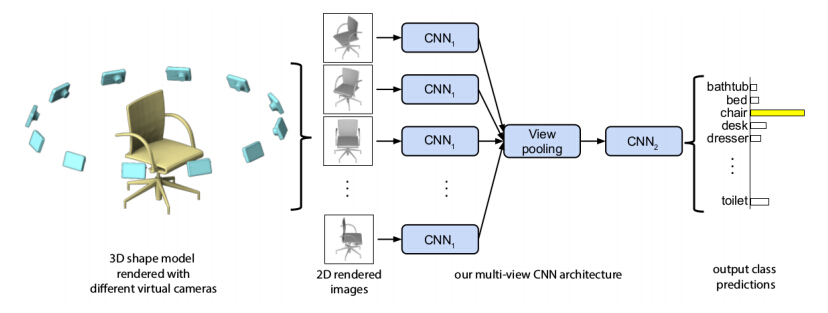
\includegraphics[width=0.98\linewidth]{figures/Su.jpg} 
\end{center} 
\vspace{-4mm}
\caption{MVCNN用于3D对象分类和检索} 
\label{fig_Su}
\end{figure}


Su等人\cite{Su2015Multi}的工作也利用了3D对象的多个视图建立一个紧凑的三维物体分类和检索任务的形状描述符。图\ref{fig_Su}所示的新型多视图CNN(MVCNN)体系结构学习了通过视图池化层将任意数量的对象输入视图组合成一个没有特定顺序的视图。为了获得不同的模型的视图,进行了两步设置。第一个设置包括通过在它们周围放置相同数量的虚拟相机来渲染3D形状得到12个视图,而第二个得到80个视图。三维模型的所有可用视图分别通过网络的第一部分,然后在视图池中的所有视图上执行元素最大池化。最后,汇总的结果通过剩余的网络传递。为了检索,网络倒数第二层(完全连接)被用作形状描述符。在MVCNN架构的实验性评估中,网络使用ImageNet1K数据集进行预训练,然后使用3D数据集ModelNet40进行微调。有关形状分类和检索的报告结果显示MVCNN优于所有其他测试方法。值得注意的是,所提出的形状描述符大大超过了Wu等人\cite{Wu20143D}最先进的3D ShapeNets的性能,特别是使用ModelNet40数据集的检索任务中。Johns等人\cite{Johns2016Pairwise}采用了一种不同的方法来开发3D对象的多个视图针对多视点物体识别在无约束摄像机轨迹下的应用场景。在这项工作中,收集的视图是组织成对,将他们的相对姿势提供给一个CNN。VGG-M网络\cite{Chatfield2014Return}在这种情况下被使用由五个卷积和三个FC层组成。灰度图像,深度图像或二者同时都可以作为网络的输入。结合来自两个图像的卷积层的输出,之后提供给第一FC层。在ModelNet数据集的实验中,这种模型超过了基于体素的3D ShapeNets\cite{Wu20143D}的性能和Su等人\cite{Su2015Multi}的MVCNN方法。

Bai等人\cite{Bai2016GIFT}提出了一种基于3D对象二维视图的实时三维形状搜索引擎。所提出的系统名为GIFT,利用GPU进行基于CNN的特征提取,并利用两个倒排文件,即一个用于加速多视点匹配过程,另一个用于重新排序初始结果。一个查询形状的检索过程能够在一秒钟内完成。作者在ModelNet、 SHREC14LSGTB\cite{Li2015A}、PSB、 McGill\cite{Siddiqi2008Retrieving}、SHREC'07\cite{Giorgi2008SHape}数据集上测试了他们的引擎,均说明了GIFT性能优于较为先进的方法,例如Chen等人\cite{Chen2003On}、Kazhdan等人\cite{Kazhdan2003Rotation}、Wu等人\cite{Wu20143D}和Su等人\cite{Su2015Multi}的方法。Wang等人\cite{Wang2015Sketch}最近提出了一种基于二维草图和二维视图检索三维模型的不同方法。更具体地说,Wang等人提出了一个体系结构,输入是一个对象的{2D视图+草图}对。该模型由两个连体CNN(即两个相同的子卷积网络)组成,一个用于处理要被检索的3D对象的2D草图,另一个用2D视图处理。两个子网分别使用SGD和反向传播进行训练。每一个子网络都包涵三个卷积层(每一个卷积层接一个maxpooling层)、一个FC层加上一个输出层。每个三维模型是被两个随机生成的视图所描述,只要他们的角度差异超过45°。该网络在三个数据集上进行了测试,并取得了最佳性能。

在Leng等人\cite{Leng20143D}所做的工作中,基于视图的深度图像也被用作输入,通过DBN提取高层抽象描述符以用于3D对象分类。DBN使用对比分散的无监督分层训练。。在从训练的DBN获得每个模型的最终表示之后,应用半监督学习方法来对每个对象进行分类。基于准确性和平均分类精度(MCP)的实验评估表明,从提出的DBN中提取的描述符导致相比于两个组合描述符合并得到相当好的结果,组合描述符结合了从不同视图提取的多个2D描述符,即CMVD\cite{Daras2010A}使用图形学习(CMVD-GL)和等权重使用图形融合(EW-GF)。Xie等人\cite{Xie2015Projective}提出了多视点深度极限学习机(MVD-ELM),并对三维形状分类和分割任务进行了测试。每个3D形状由20个2.5D深度图像/投影的集合表示,所述图像/投影使用以每个对象为中心的球体均匀地捕捉。MVD-ELM模型包含卷积层和pooling层。每个卷积层的权重在所有视图之间共享。输出权重根据提取的特征映射进行优化。该模型的完全卷积扩展(FC-MVD-ELM)也被用于三维形状分割任务。这个网络只包含两个卷积层,没有任何pooling层。使用实例的多视点深度图像训练FC-MVD-ELM。然后,将所有预测的标签投影回原始3D网格。最后,使用图形切割优化来平滑分割结果。所提出的模型优于其他相关方法(例如Wu等人\cite{Wu20143D}),并显着减少了训练时间。

受到多视点深度神经网络效果优于采用三维形状的全部三维信息的启发,最近在Qi等人\cite{Qi2016Volumetric}中提出了用于目标分类的体视图与多视图CNN的最近的研究和比较。对于多视图CNN的情况,Qi等人提出了球形渲染,即多分辨率3D滤波以利用多尺度的信息,并结合训练数据增强来实现对已经高性能的MVCNN在ModelNet40数据集上的增强。


\section{DL架构作用于超光谱数据}

先进的遥感技术目前已经被用于多个方面。通常使用机载或星载传感器来捕获超光谱(HS)图像,一般以N个大小为[p1×p2]图像堆叠来表示各个频带的辐射大小,因此也被称为3D超立方体,该方法在Bioucas-Dias等人的文章中可以看到\cite{Bioucas2013Hyperspectral}。传统的HS数据分析方法利用了光谱信息,但也有提出了同时处理光谱和空间数据的方法。最近,应用于HS数据的DL方法开始出现,显示广泛的前景。在Zhang等人\cite{Zhang2016Deep}的研究中,可以找到关于使用遥感数据解决图像预处理,基于像素的分类,目标识别和场景理解的最新DL方法的详细技术教程。在所提到的任务中,基于像素的分类可能是应用最为广泛的。

\begin{figure}[tb]
\begin{center}
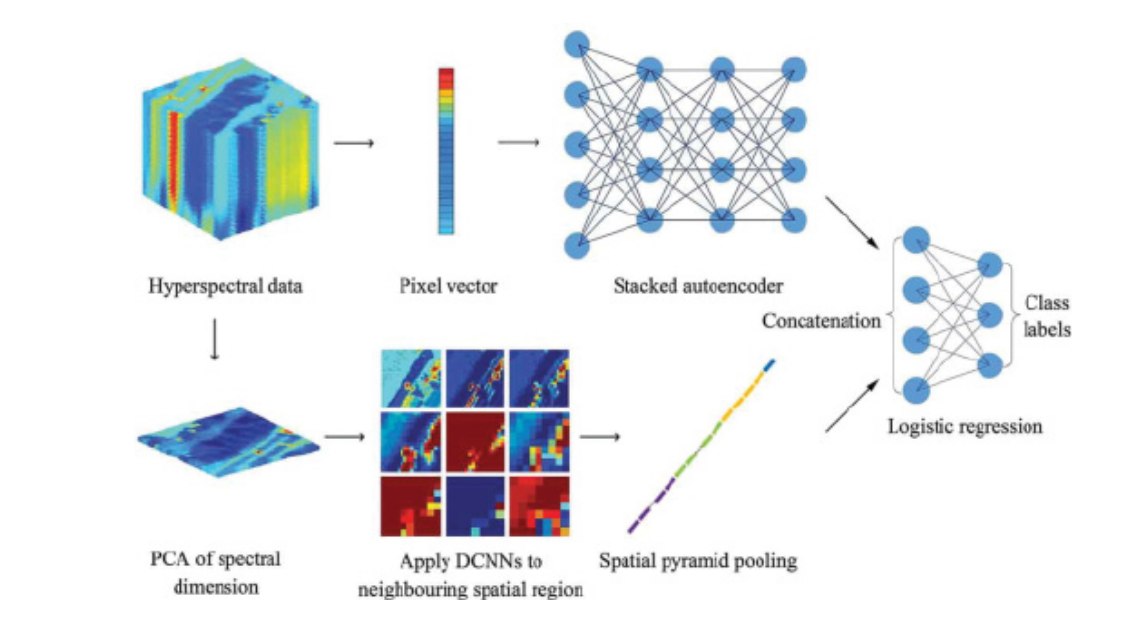
\includegraphics[width=0.9\linewidth]{figures/Yue.png} 
\end{center} 
\vspace{-4mm}
\caption{Yue等人的联合光谱与空间信息的分类框架} 
\label{fig_Yue}
\end{figure}


针对深部高光谱数据分类,Hu等人\cite{Hu2015Deep}采用CNN直接在谱域进行分类。所提出的架构由输入层(接受具有每个像素的频谱的矢量),卷积层,最大池层,FC层和输出层组成。与基于SVM的分类器和其他CNN体系结构相比,作者所提出的方法能够得到更好的结果。在Chen等人\cite{Chen2017Deep}的工作中,其利用堆积AE(SAE)从高光谱数据中提取深度特征来进行分类。作者尝试了两种框架:第一种是利用光谱或空间特征,第二种是基于联合光谱和空间信息特征的分类。具有像素谱的矢量作为AE的输入提取谱特征,而从原始图像中提取特定像素的[n×n]相邻区域并将其作为输入提供给用于空间区域的深度模型得到空间特征。实验结果表明,深度模型比标准SVM分类器表现更好,同时融合光谱特征与空间特征的深度框架比仅使用光谱或空间信息的版本更胜一筹。Chen等人\cite{Chen2015Spectral, Chen2016Deep}提出的类似框架,分别使用DBN和3D CNN的方法也证实了这一观点。Makantasis等人\cite{Makantasis2015Deep}也提出了基于DL的分类方法,其基本思想是利用CNN从光谱和空间数据中提取特征表示。设计的网络包括两个卷积层,而多层感知器用于分类。所提的方法与基于SVM的分类器进行比较,具有明显优势。

Zhou和Wei\cite{Zhou2016Learning}引入了一个称为频谱空间网络(Spectral-Spatial Network,SSN)的分层模型来处理HS图像分类。该网络由几个叠加的光谱空间特征学习单元(SSFLUs)和一个顶层的基于核的极限学习机(KELM)\cite{Huang2012Extreme}组成,并且用于分类。每个SSFLU包括用于提取判别性频谱特征的LDA步骤和用于利用空间信息的自适应加权滤波器(AWF)的应用。与其他最先进的方法相比,实验证明了SSN具有更为良好的准确性和鲁棒性。Zhao和Du\cite{Zhao2016Learning}采用多尺度CNN。该方法首先利用PCA进行降维,然后在三个PC频带上进行特征提取。为每个选定的PC波段构建一个图像金字塔,以多尺度捕捉空间特征。利用Logistic回归(LR)分类器将空间和谱特征相结合来对每个PC带进行分类,而采用投票方案来融合所有谱带的分类结果。作者比较了提出的方法与扩展形态概况(EMPs)\cite{Benediktsson2005Classification}和复合核SVM\cite{Fauvel2012A},并指出其有效性。在Yue等人\cite{Yue2016A}的工作中,空间金字塔池化(SPP)被用于HS图像分类。如图\ref{fig_Yue}所示,DL框架包括将叠加的AE的输出与CNN和softmax分类器组合在一起的特征提取。SPP被应用在深CNN的最后一个卷积层之后,允许产生固定长度的特征而不管输入特征的规模如何。 实验评估结果表明,与RBF-SVM和EMP-SVM相比,该方法性能优越。

\section{总结}
在过去的几年中,DL方法已经被设计并成功应用于一维和二维数据。然而在3D领域使用它们并不那么简单,因为典型的DL架构被设计为将1D或2D数据作为输入。为了克服这个障碍,已经提出了几种方法。在本节中,对于在将数据提供给DL架构之前处理3D数据的方式或者对DL架构进行修改以直接采用3D数据作为输入的方式来识别并分别分析了五个类别。为了处理3D数据,许多研究人员利用了特征工程的进步。低级特征提取已被用于多个计算机视觉任务中,取得了巨大成功,迄今为止已经提出了大量的局部或全局描述符用于3D数据。由于低级描述符通常不足以表征3D对象的高级语义,因此该技术将其与深度模型结合使用,以提取高层描述符。然而,考虑到3D数据的复杂性,这种表示可能缺乏区分能力,因为低层表示可能从3D表示中省略重要的信息。另外,RGB-D传感器的应用能够提供额外的深度模式(除标准RGB通道外),其中包含有关3D对象形状的重要信息。大多数研究者分别处理颜色和深度通道(即图像),而其他人仅使用深度信息来设计他们的系统。这些传感器的巨大优势在于它们对普通用户而言是便宜的,同时还有许多开源软件解决方案可以帮助他们使用。然而,它们的低成本往往与噪声和不完整的捕获数据相结合,可能使得它们不适用于复杂的情况。一些最近的工作已经尝试通过用三维卷积层替换二维卷积层来直接利用三维信息。 3D体积模型提供了丰富而强大的3D形状表示,包括所有重要的细节。尽管在计算硬件方面取得了巨大的进步,但是它们的处理在内存和计算时间方面仍然是要求很高的。结果,低分辨率只被使用到目前为止。其他研究人员从不同的角度来解决这个问题,并利用从不同视点(多视图)捕获的场景的一个或多个2D视图。通过这样做,问题被间接地转换到图像域,因此基于多视图的方法可以利用图像处理的最新进展,并且可以直接使用。然而,它们的使用引起了一些问题:(1)在2D视图中丢失了3D形状的完整的三维几何信息,(2)3D形状的视图的数量以及链接的方式是非常关键的一步,能够影响所提出的方法的效率和有效性。


% 第三章


\chapter{基于多模态深度学习的三维形状识别与检索}

在本文中,我们提供了一个综合考虑三维形状的外在属性和内在特征的解决方案。 我们提出了一个新的方案来融合3D形状的不同形态数据到深度学习框架。 其核心思想是运用深度学习技术,融合三维模型的几何特征和视觉特征,并进行提取得到具有强表达能力的高层特征。简而言之,卷积深度置信网络(CDBN)和卷积神经网络(CNN)分别用于从基于几何的模态和基于视图的模态学习三维形状。 接下来,这两种模式利用受限玻尔兹曼机(RBM)融合以获得具有更强判别力特征。其中包括以下三个主要部分:
\begin{enumerate}
\item 基于视觉的特征学习
\item 基于几何的特征学习
\item 多模态融合
\end{enumerate}


这个框架有三个好处,如下所述。 首先,融合不同的模式,可以全面理解3D形状。 第二,在不同的特征提取程序中使用不同的深度学习技术,充分利用各种深度学习方法从三维模型中提取不同特征的属性。 第三,与其他需要手动调整参数以获得最佳性能的机器学习方法不同,在整个学习过程中没有要调整的参数。 提出的方案是自动学习的。

尽管上述方法在分类,匹配和检索方面取得了巨大的进步,但是在更多领域应用3D对象还远远不能令人满意。主要问题在于基于几何的方法和基于视图的方法仅使用3D对象的部分信息。 详细而言,基于几何的方法利用了3D模型本身的复杂拓扑结构和几何特性,而忽略了三维物体之间的视觉相似性。 相反,基于视图的方法仅考虑来自不同观看图像的模型的视觉特性。 为了克服各自缺点,我们尝试使用深度学习技术来学习和融合几何和视图方面的不同模式。 这项工作的主要贡献可以归结为两个方面:
\begin{itemize}

\item 多模态融合:为了进一步提高性能,采用多模态融合学习三维形状内在的非线性关系。 通过融合多模描述符,可以封装互补的视觉和几何信息,提高分类和检索的准确性。
\item 深度特征:CNN和CDBN用于提取3D形状的视觉和几何特征。 CNN具有较强的视觉特征提取能力,而CDBN具有从3D对象中产生高性能特征的能力。我们的框架充分利用了CNN和CDBN,因此可以提取更全面的描述。

\end{itemize}



\begin{figure*}[htbp]
\begin{center}
 \includegraphics[width=0.98\linewidth]{figures/cnn-cdbn-dbn-crf-new14}
 \end{center} \vspace{-4mm}
\caption{基于多模态深度学习的三维形状识别与检索的流程图(展示了离线的训练过程)% The multi-modal feature data association part is detailly shown in Fig. \ref{fig_multi-modal_structure})
} 
\label{flowchart}
\end{figure*}

几何和视觉信息是三维形状研究的两个重要方面。在我们的框架中,我们分别提取这两个类型的描述符,然后将它们融合生成具有高判别性和有效性的3D MMF。该方法的流程图如图\ref{flowchart}所示,表明提出的多模态特征融合体系结构包含两个模态输入:几何描述符和视觉描述符。传统的几何特征是使用复杂的三维形状结构应对大量丰富点设计的。在预处理中下采样是减少产生各种特征的计算时间的有效方法。在我们的框架下,CNN和CDBN模型的预处理是没有下采样方法产生的体素化和深度图像。在几何特征提取中,三维形状从网格形式转换成接近原始三维对象的体素表示,因此我们不需要下采样。在视觉特征提取中,我们以深度图像作为输入,由于将三维形状转换为多幅图像,也不需要下采样。接下来分步介绍。


\section{所涉及的深度学习方法介绍}

\subsection{卷积神经网络(CNN)}

卷积神经网络(CNN)是一种有效的模式识别领域的方法。传统模式识别的方法中,图像的预处理是一件非常复杂的事情,例如,平滑,锐化等操作,因此增加了图像处理的复杂性,效率不高。CNN可以直接对图像进行处理,其区域连接和权值共享更是提高了CNN的图像处理的能力,加了整个模型的计算性能。CNN如此优秀的表现,得益于Hubel和Wiesel的贡献。他们发现在猫脑皮层中用于局部敏感和方向选择的神经元有这种区域连接的网络,不仅有效地降低反馈神经网络的复杂性而且增加了预测的精度。

% 卷积神经网络是近年发展起来,并引起广泛重视的一种高效识别方法。20世纪60年代,Hubel和Wiesel在研究猫脑皮层中用于局部敏感和方向选择的神经元时发现其独特的网络结构可以有效地降低反馈神经网络的复杂性,继而提出了卷积神经网络(Convolutional Neural Networks-简称CNN)。现在,CNN已经成为众多科学领域的研究热点之一,特别是在模式分类领域,由于该网络避免了对图像的复杂前期预处理,可以直接输入原始图像,因而得到了更为广泛的应用。 K.Fukushima在1980年提出的新识别机是卷积神经网络的第一个实现网络。随后,更多的科研工作者对该网络进行了改进。其中,具有代表性的研究成果是Alexander和Taylor提出的“改进认知机”,该方法综合了各种改进方法的优点并避免了耗时的误差反向传播。

CNN神经网络作为第一个被成功训练并且应用的多层神经网路结构,具有较强的容错、自学习以及并行处理能力。最初是为识别二维图像而设计的多层感知器,模仿生物神经网络的局部链接和权值共享网络降低了神经网络的复杂度,减少权值数量,使网络对于输入具备一定的鲁棒性。CNN是一种多层的神经网络,具有很强的抽取图像特征能力,其网络结构具有很强的自学习和并行处理的能力。1962年Hubel和Wiesel通过对动物的视觉皮层细胞进行研究,提出了感知域的概念,用以能够使得神经元收到刺激而进行反馈的区域,同时这也说明一点,神经元的最初感知是发生在局部区域的。后续的相关研究相继提出简单单元(Simple Cell)和复杂单元(Complex cell)。简单单元只对方向的边缘产生响应,复杂的单元除了对方向的边缘产生响应,而且具有一定的空间不变的属性。基于感知域,神经认知机模型被提出,并且将其应用于计算机视觉中的视觉模式分类任务。神经认知机首先用多个模式来表示一个模式,接着以分层的方式对这些模式进行处理,通过不断的尝试将该视觉模型化,让其能够应对物体的偏移、扭曲等变形的识别。

基于认知机模型,世界的各地研究者提出了多种卷积网络形式用于视觉分类与识别。近年来,Yann LeCun教授提出的卷积神经网络是当前最为流行的一种形式,该网络成功应用于语音识别和图像分类等问题,推动了深度学习的发展。 CNN在神经网络的基础上,采用了局部感知野和权值共享的思想,有效地降低了传统前馈神经网络的复杂程度,并使用降采样层(又称作pooling层)来增加网络的平移不变性。

\textbf{CNN基本网络结构} 

卷积神经网络是一种多层的前馈网络,每一层由多个二维平面组成,每个平面再由多个神经元组成,如图\ref{cnn}。网络中卷积层(Convolutional Layer,C)和抽样层(Subsampling Layer,S)交替出现,相当于生物视觉系统中的简单单元和复杂单元交替出现。网络的最后一层为全连接方式的神经网络,输出层的维度对应数据中需要进行分类的类别数。

卷积层:该层为网络的特征提取层,每个卷积层包含多个神经元(C),每个神经元只对前一层的网络相应的局部位置进行特征提取,这体现在该神经元与前一层局部区域的连接权重上。相比较全连接的神经网络模型,这种局部连接的方式可以大大降低整个网络的参数。为了更加有效的训练整个网络,整个网络设计时采用权值共享的基本策略:即神经元对同一层所有区域的感知权值是相等的。特征映射结构采用Sigmoid函数作为卷积网络的激活函数,使其具有位移不变性的特点。

抽样层:该层为网络的特征映射层,每个卷积层包含多个神经元(S),网络的每个计算层由多个特征映射组成,每个特征映射为一个平面,平面上所有的神经元权值相等。
通过卷积层(C-层)和采样层中(S-层)交替进行特征提取,使得训练出来的特征对输入数据具有很高的畸变容忍能力。

\begin{figure*}[htbp]
\begin{center}
 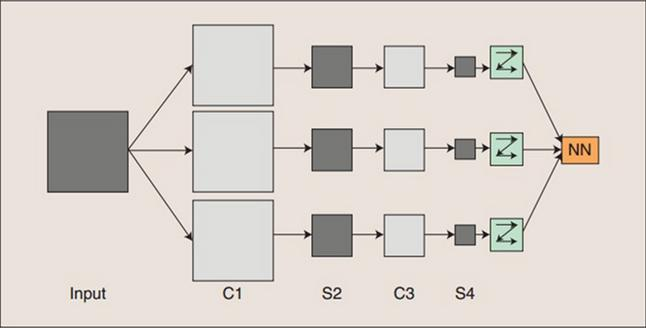
\includegraphics[width=0.98\linewidth]{figures/cnn}
 \end{center} \vspace{-4mm}
\caption{卷积神经网络结构} 
\label{cnn}
\end{figure*}



\textbf{CNN训练学习} 

\begin{enumerate}
\item \textbf{卷积层。} 图像本质是一种由像素值排列起来的二维(或者多维)矩阵,是现实世界的一种数字化表现形式。由于图像的统计特性是有一定规律的,在图片中某一区域学习得到的局部特征同样能应用于另一区域。图\ref{conv}展示了图像卷积的过程。 

\begin{figure*}[htbp]
\begin{center}
 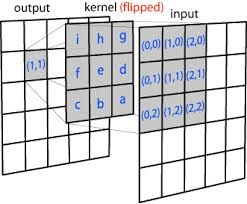
\includegraphics[width=0.5\linewidth]{figures/卷积过程}
 \end{center} \vspace{-4mm}
\caption{图像卷积过程} 
\label{conv}
\end{figure*}

在CNN网络中,原始输入图像(或者特征图)$x$ 经卷积核$W$ 处理之后,会生成新的特征图,此过程能够表示为
\begin{equation}
 I = f(x \otimes W)
\end{equation}
式中, 为$\otimes $为卷积操作, $I$为卷积单元处理后的结果, $f$为非线性变换函数。

\item \textbf{池化层降采样过程。} 该层对卷积层所产生的特征图进行下采样操作, $N$个输入特征图对应$N$个输出特征图,只是每个输出特征图的尺寸相比较原来变小,抽样层定义如下:

\begin{equation}
  a_j^l  =\sigma (\beta_j^l down(a_j^{l-1}) + b_j^l)
\end{equation}

公式中$down()$为下采样操作,对输入图中每个不重复的$n\times n$ 得图像块求和得到一个输出值,输出图的长和宽都是输出图的$1/n$ ,每个输出有一个乘性偏置$\beta$ 和偏置$b$ 。只要得到抽样层的灵敏度图,就可以求解出偏置参数$\beta$ 和偏置$b$的梯度。

卷积操作虽然能够有效降低整个网络的参数,但是对于图像处理来说,参数量仍然非常巨大。CNN有一个巧妙的安排,在卷积之后再进行池化操作。池化操作是对卷积出来的特征进行聚合的,从而进一步降低参数的个数。一般来说,最大池化、均值池化、随机池化是比较常见的。池化的作用不仅能降低维度而且能防止过拟合的作用,使特征具有平移鲁棒性。

% 通过卷积的方法得到输入图像的特征图之后,可以利用这些特征完成各种计算机视觉的任务。但如果直接使用这些特征图,会使得特征的维度非常高,训练一个高维度输入的模型十分不方便,而且容易出现过拟合。为了解决上面这个问题,可以对图像中某一区域的特定特征进行聚合操作,称之为池化(pooling),这种做法可以降低特征的维度,同时还能在一定程度上改善过拟合。常用的池化方法有最大值池化、均值池化和随机池化几种方法,其中最大值池化方法在卷积神经网络中应用较广。卷积操作之后进行降采样的做法,是CNN模型的显著特点。卷积层的功能为从原始图像中捕捉特征信息,减少无效信息的强度,而降采样层的功能是负责降维,减小计算量,同时保证了原始图像的平移鲁棒性。

\item \textbf{CNN的优势。} 在图像的识别处理过程中,传统的神经网络对图像的处理是使用全链接的。全链接得的最大的弊端就是需要学习的参数特别巨大,例如$1000 \times 1000$ 的图像,如果与$10^6$的隐藏层节点进行全链接,那么参数的数量将是成指数级别进行上涨的,那是将会有$10^{12}$个参数。面对如此巨量的参数,传统的神经网络难以进行有效的学习。CNN的卷积操作弥补这一弊端,CNN提出了区域连接和权值共享这两个技术。区域连接指神经网络的不是所有节点进行连接的,而是选择部分区域进行,这样有效的减少了参数,但同时CNN会在高层的时候对这些局部参数进行融合,进而弥补部分区域的信息的缺失,同时权值共享使得卷积核对不同的区域所有的参数可以共享,对于提取出来的参数不同部分是可以共享的。CNN使得对图像的处理效率更高,效果更好。

%由于传统的前馈神经网络全连接特性,当用于处理图像数据时,计算量是十分巨大的。比如一幅 $1000 \times 1000$ 的图像,将其转化为像素的一维向量后,将含有 $10^6$个元素,如果隐藏层节点数目也为 $10^6$,那么单层神经网络的参数数量就为 $10^12$个,这样巨大的参数个数会导致整个神经网络无法训练。为使神经网络算法对图像可用,必须减少网络中权值边的个数,CNN使用区域连接和权值共享思想来达到这一目的,这两种方法可以有效减少网络中的连接边数,区域连接和权值共享等价于CNN中的卷积层操作。换角度看,CNN中的卷积层操作实质上是区域连接和权值共享思想的具体实现。
%局部连接是指网络中的任意节点并不一定要与前一层的所有节点都有权值边相连,有可能只与部分节点相连接,只对图像的局部特性进行处理,在更高层中完成对图像区域信息的整合,就可得到图像的全局信息。在图像中某一部分学习得到的特征同样能应用于图像中其它部分,这就是连接边权值共享的基本原理。权值共享使得在CNN的每一个特征图(或者原始图像)内部,所有与卷积核大小相同的图像块所对应的连接边权值是完全一样的。对于CNN模型来说,区域连接和权值共享策略降低了网络训练的难度,使得训练一个有效的多层CNN网络具备了可能性。

\end{enumerate}

\subsection{深度置信网络(DBN)}
深度置信网络DBN是一种全连接网络,网络的训练过程就是优化其能量函数达到最小的过程。波尔兹曼机(BM)是一种非监督学习技术,常常被用作数据挖掘方面的处理。但是由于其隔层的节点之间的进行了层内的连接,使得BM的训练学习效率低,使得这种方法难以被广泛应用。Smolensky为了解决其效率低下的问题,将层内节点之间的连接全部去掉,提高了网络的学习效率,同时层间之间全链接,这种神经网络被称为限制性波尔兹曼机(RBM)。

RBM包含可使层、隐藏层,层内无连接,层间全链接。当隐藏层神经元足够多的时候,RBM可以拟合离多数散分布。RBM的提出是对BM的一个重大进步,然而,RBM还是没有得到广泛应用。究其原因,就是训练的时候仍然有诸多困难,进而难以高效的训练神经网络。Hinton针对这种问题,提出对比散度(CD)算法。有效的解决了RBM不能高效训练的问题,使得其在分类、回归、降噪、高维时间序列分析、图像特征提取、协同过滤等方面取得了优秀的表现。Hinton在对RBM研究的基础上,又提出了将多个RBM进行堆叠的想法,进而提出了深度信念网络(DBN),DBN的提出为神经网络参数的初始化提供了有力的工具。

% 这类网络首先起源于Holpfield网络,这是一种全联接的网络,神经元之间进行全连接,我们可以给这个网络定义一个能量函数,神经网络的学习任务就是使能量函数达到最小值。这类网络典型的成功应用是担货郎问题,即有N个地点,每个地点间都有道路相通,担货郎必须把货物送到每个地点,通过Holpfield网络,可以有效地找到最佳路径。但是即使是对于二值(神经元只能处在0或1状态),全联接网络的状态也2的N次方个状态,要从这些状态中找到找到能量函数的最小值,难度相当大,大家一定还记得国际象棋发明者,向国王讨赏的典故吧,一个64个方格的棋盘,连全世界总粮食产量都填不满,可见这个问题的复杂性。与此同时,根植于统计力学模型的波尔兹曼机(BM)也开始流行起来。在这种网络中,神经元的输出只有激活和未激活两种状态,用0或1来表示,各个神经元的输出值由概率纺计模型给出。

%由实践来看,波尔兹曼机(BM)具有强大的非监督学习能力,可以发现数据中潜在规则,理论上来讲,非常适合于数据挖掘领域应用。便是由于是全连接网络,导致这种网络的训练时间非常长,没有高效的学习算法,直接制约了这种网络的应用。后来Smolensky引入了限制性波尔兹曼机(RBM)模型,其主要思想就是去掉了波尔兹曼机中层内连接。限制性波尔兹曼机(RBM)具有一个可见层,一个隐藏层,层内神经元间无连接,层间神经元全连接。

%限制性波尔兹曼机(RBM)中,输入信号通过可见层输入到网络中,此时传播到隐藏层后,各隐藏层神经元的激活是互相独立的,同理在给定隐藏层信号后,反向传播到可见层时,可见层神经元的激活也具有独立性。可以从理论上证明,这种网络结构,只要隐藏层神经元节点足够多,限制性波尔兹曼机(RBM)可以拟合任意离散分布。虽然在理论上RBM很好,但是一直由于没有高效的学习算法,限制性波尔兹曼机(RBM)并没有得到广泛应用。但是深度学习之父Hinton在2002年提出了对比散度(CD)算法,使限制性波尔兹曼机(RBM)具备了快速学习的能力。从此,RBM得到了广泛的应用,出现了各种对比散度算法的变种,使得算法收敛性更高。与此同时,波尔兹曼机(RBM)在分类、回归、降噪、高维时间序列分析、图像特征提取、协同过滤等方面,得到了广泛的应用。另外,Hinton在2006年提出,将限制性波尔兹曼机(RBM)堆叠起来,形成深度信念网络(DBN),通过逐层训练RBM网络,将训练好的RBM网络堆叠成深度学习网络,可以得到非常好的初始参数值,有效地解决了大型神经网络训练速度慢的问题,是当前的研究热点之一。

\textbf{受限制的玻尔兹曼机RBM}

之所以说他是受限,是应为在RBM内取消了可见层和隐含层的层内连接,虽然BM具有强大的无监督学习能力,能过学习复杂的规则,但是因为层内连接,使得整个学习过程消耗漫长的时间。所以Smolensky发明了RBM是学习时间大大缩减。也为后面的DBN奠定了基础。

RBM有一个可见层和一个隐含层,通过上面的BM到RBM的转变使得RBM具有了一个很好的特性:在给定可见层单元状态时,各隐含单元的激活条件独立,反之,在给定隐含层单元的状态时,各隐含层激活条件也是独立的。虽然这样RBM所表示的分布仍是无法有效计算的,但是我们可以通过Gibbs采样使其得到服从RBM分布的随机样本。

RBM的可见层用v表示,用于接收输入信号,隐藏层由h表示,可以视为是输入信号的特征提取器。我们在前面讨论过,制约神经网络大规模应用的一个瓶颈之一,就是很难为研究问题找到合适的特征,而RBM则是通过无监督学习方式,自动找到研究问题的最佳特征,因此对于研究者们而言,具有非常大的吸引力,这也是为什么RBM在近些年来如此火的原因。我们设定可见层神经元为二值变量,即,隐藏层单元同样为二值变量,即,假定可见层有m个神经元,用下标i代表第j个神经元,隐藏层有n个神经元,用下标j表示第j个神经元。

我们可以定义网络的能量函数为
%
\begin{equation}
 E(v,h|\theta) = - \sum_{i=1}^n \sum_{j=1}^m v_jW_{ij}h_i - \sum_{j=1}^m b_j v_j - \sum_{i=1}^n c_i h_i,
\end{equation}
%
上式中为网络参数,均为实数,$W_{ij}$为可见层神经元i到隐藏层神经元j的连接权值,$b_j$为可见层第j个神经元的偏置,$c_i$为隐藏层第i个神经元的偏置。


\textbf{深度信念网络}
在机器学习的模型分类中,大抵可以分为两类,生成模型和判别模型。简单来说,生成模型刻画的是数据和标签的联合分布,而判别模型对于由数据预测类别进行了刻画。传统DBN进行训练的时候,弊端很多。例如,样本集标签必不可少,收敛慢,可能会收敛与局部最优等等问题。

DBNs由多个限制玻尔兹曼机(Restricted Boltzmann Machines)层组成。这些网络被“限制”为一个可视层和一个隐层,层间存在连接,但层内的单元间不存在连接。

% 隐层单元被训练去捕捉在可视层表现出来的高阶数据的相关性
% 首先,先不考虑最顶构成一个联想记忆(associative memory)的两层,一个DBN的连接是通过自顶向下的生成权值来指导确定的,RBMs就像一个建筑块一样,相比传统和深度分层的sigmoid信念网络,它能易于连接权值的学习。在最高两层,权值被连接到一起,这样更低层的输出将会提供一个参考的线索或者关联给顶层,这样顶层就会将其联系到它的记忆内容。而我们最关心的,最后想得到的就是判别性能,例如分类任务里面。
% 
% 在预训练后,DBN可以通过利用带标签数据用BP算法去对判别性能做调整。在这里,一个标签集将被附加到顶层(推广联想记忆),通过一个自下向上的,学习到的识别权值获得一个网络的分类面。这个性能会比单纯的BP算法训练的网络好。这可以很直观的解释,DBNs的BP算法只需要对权值参数空间进行一个局部的搜索,这相比前向神经网络来说,训练是要快的,而且收敛的时间也少。

卷积置信网络CDBN(Convolutional Deep Belief Networks)是DBN网络的拓展之一。DBN在图像训练的过程中,仅仅对原始数据进行向量化,即就是将二维化的图像信息转化为一维的向量信息。这种操作很明显的一个弊端就是丢失了二维图像信息的空间结构化信息。为了弥补这方面的不足,CDBN别来学习图像信息的结构化信息,卷积操作对于原始数据不仅仅是学习其直接表达,跟能够学习不同像素之间的位置关系。因此,同时CDBN的卷积操作也具有区域连接和权值共享的优势,对于训练数据量巨大的数据集有着不DBN更大的效率优势。

% DBNs的灵活性使得它的拓展比较容易。一个拓展就是卷积DBNs(Convolutional Deep Belief Networks(CDBNs))。DBNs并没有考虑到图像的2维结构信息,因为输入是简单的从一个图像矩阵一维向量化的。而CDBNs就是考虑到了这个问题,它利用邻域像素的空域关系,通过一个称为卷积RBMs的模型区达到生成模型的变换不变性,而且可以容易得变换到高维图像。DBNs并没有明确地处理对观察变量的时间联系的学习上,虽然目前已经有这方面的研究,例如堆叠时间RBMs,以此为推广,有序列学习的dubbed temporal convolutionmachines,这种序列学习的应用,给语音信号处理问题带来了一个让人激动的未来研究方向。




\section{基于几何的特征学习}
传统的几何描述符是使用具有人类先验知识的复杂三维形状结构设计的,这增加了设计师处理各种应用中使用的大量3D形状的工作量并降低了效率。 CDBN由于其是无监督和深度的学习网络,是一种自动学习高判别性特征的强大工具。 3D形状由复杂的拓扑结构构成,CDBN似乎很难直接用于三维形状分析。 因此,我们首先将三维形状离散化为正则化网格,并将其体素化作为三维CDBN的输入来提取几何描述符。

\subsection{体素化}
体素化是将三维形状网格形式转换为接近原始三维对象的三维像素表示。 其不但含有模型表面的信息,还刻画了模型的内在结构属性。 这种表示方式是保留一定的重要几何信息的一种空间关系,离散化了三维模型,减少了原有的复杂三维结构,便于三维CDBN提取内在的三维几何特征。 我们使用二值化三维矩阵来表示三维形状的几何信息。 在3D矩阵中,如果一个体素在3D网格内,则表示形状分布概率的相应矩阵项目被设置为1; 否则将概率值设为0.然后我们以3D矩阵作为CDBN的输入来提取几何描述符。 在这项工作中,我们扩展了CDBN实现来支持3D数据。

\subsection{几何描述符}
对于二维图像,DBN\cite{Hinton2006A}是一个强大的概率模型,用于模拟像素和标签上的联合概率分布。 然而,将模型从2D像素数据适配到3D体素数据是一个挑战。 具有合理分辨率的三维像素体积比具有普通尺寸的图像具有更大的数据,并且在完全连接的DBN中存在大量的参数,这使得模型难以被有效训练。 所以我们使用卷积来减少模型参数的权重分享。 与传统的卷积深度学习相比,我们忽略了可能给特征生成带来更大不确定性的pooling层。

在我们的模型中卷积层的能量被定义为:
%
\begin{equation}
 E(x,h) = - \sum_{f} \sum_{j} \left( h^f_j \left( W^f * v \right) + c^f h^f_j \right) - \sum_{l} b_l v_l ,
\end{equation}
%
其中$ v_l $表示每个可见单元,$ h ^ f_j $表示特征通道$ f $中的每个隐藏单元,$ W ^ f $表示卷积滤波器。 “*”符号表示卷积操作。 在这个能量定义中,每个可见单元$ v_l $与一个唯一的偏差项$ b_l $相关联,以便于重建,同一个卷积通道中的所有隐藏单元$\{h^f_j\}$共享相同的偏差项$ c^f $。 类似于\cite{krizhevsky2012imagenet},我们也允许一个卷积步长。

\begin{figure*} [htbp]
\begin{center}
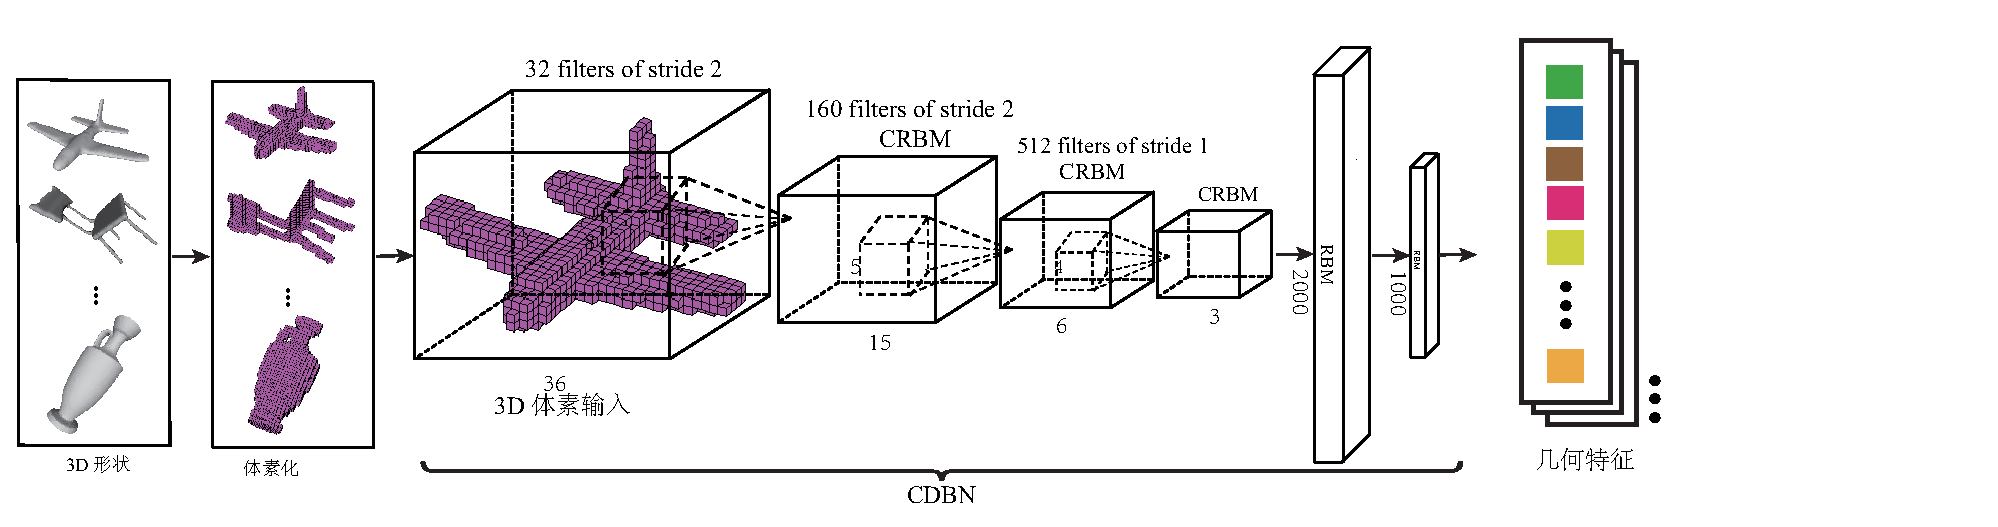
\includegraphics[width=0.98\linewidth]{figures/3d_cdbn}
\end{center} 
\vspace{-4mm}
\caption{我们的3D形状CDBN结构,为了说明方便我们对每个卷积层只画了一个滤波器。}
\label{fig_CDBN_shape}
\end{figure*}


我们将三维形状设置为30×30×30的三维像素网格,并在两个方向上都有3个额外的填充单元,以减少卷积边界伪影。 我们提出将标签看作是softmax变量的标准变量之一。 我们模型的最终体系结构如图\ref{fig_CDBN_shape}所示。第一层有32个尺寸为8,步幅为2的滤波器; 第二层有160个尺寸为5和步幅2的滤波器; 第三层有512个尺寸为4的滤波器; 每个卷积滤波器连接到前一层的所有特征通道; 第四层是一个标准的全连接RBM,有2000个隐藏单元; 具有1000个隐藏单元的第五层和最后一层以多项式标签变量和伯努利特征变量的组合作为输入。

3D CDBN模型经过两个步骤的训练,包括分层预训练和生成微调程序。在预训练过程中,前四层采用标准对比散度算法\cite{Hinton2002Training}分别进行训练,顶层采用快速持续对比散度(FPCD)训练\cite{Tieleman2009Using}。一旦下层被学习,权重是固定的,隐藏的激活被输入到下一层作为输入。在我们的微调程序中,我们采用类似于唤醒睡眠算法的方法\cite{Hinton2006A}。在唤醒阶段,我们自下而上传播数据,并使用激活来收集正面的学习信号。在睡眠阶段,我们在最顶层维护一个持续链,并自上而下传播数据以收集负面的学习信号。这个微调程序模仿了模型的识别和生成行为,在实践中运行良好。一旦整个网络的权重已经被学习,我们利用输入的体素化数据使用正向计算生成几何描述符 $o(\mathbf{X}_{shape})$。



\section{基于视觉的特征学习}

从图形角度分析三维模型的常用方法是将三维模型从不同角度转换成二维图像。理论上,这些二维图像应尽可能包含来自三维模型的信息。 在我们的视觉描述符生成过程中,我们首先将3D形状从20个方向投影到2D图像中,并采用CNN进一步提取视觉特征。 我们的算法的细节总结如下。

\subsection{3D模型预处理}
在这一部分,我们将原点设置在三维模型的质心,然后测量点到其表面的最大极距。其中旋转归一化没有执行,但是这将在之后一定程度上被补偿。

\subsection{深度图像的采集}

深度图像,一种二维图像,来自于从质心居中的正十二面体的20个顶点的虚拟相机的拍摄。在所提出的方法中,我们旋转正十二面体10次以使该特征对旋转具有鲁棒性。应该仔细设置旋转角度,以确保所有相机均匀分布,并能够覆盖3D模型的不同视角。 我们认为十二面体有20个顶点可以产生中等数据量,从而保证高计算性能和重要的信息。 该策略与LFD在视图提取方面类似,但略有不同,我们丢弃二值图像,只使用二维深度图像。 最后一个3D模型由200个图像表示,每个图像的大小为256×256。

在深度图像渲染中,有效信息集中在图像的中心。 因此,我们移除深度图像的边界,并将图像从256×256裁剪成124×124的大小,以滤除干扰和冗余信息,从而使数据紧凑。 另外,由于图像尺寸小于原始深度图像,该处理可以促进之后的CNN特征学习。 因为CNN模型的有效输入范围是从0到1,所以深度图不适合作为CNN模型的输入。 因此,我们将每个维度的范围标准化为[0,1]。

\subsection{视觉描述符}

\begin{figure*}[htbp]
\begin{center}
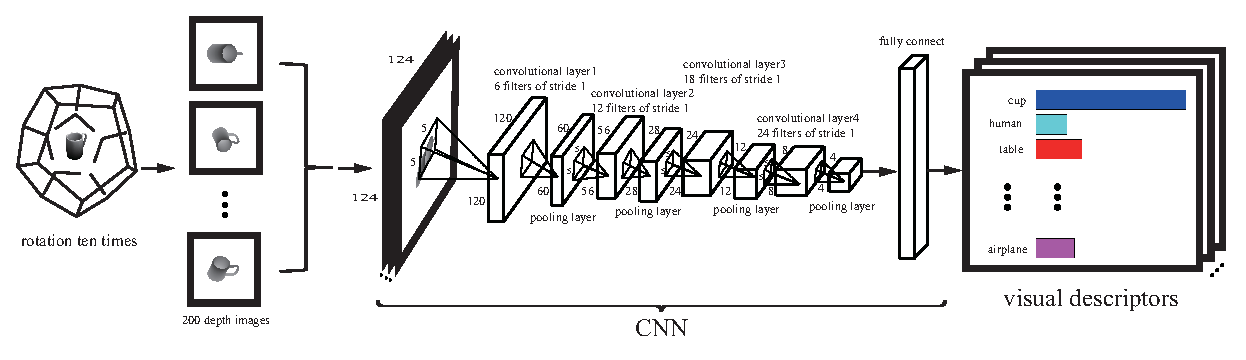
\includegraphics[width=0.98\linewidth]{figures/view_cnn7}
\end{center} 
\vspace{-4mm}
\caption{我们的三维形状CNN模型,为了说明方便我们对每个卷积层只画了一个滤波器。} \label{fig_CNN_view}
\end{figure*}

CNN已经比较成功的应用于图像处理。从上面的程序中,我们获得包含丰富的关于3D模型的视觉信息的2D图像。 因此,CNN被用来提取3D形状的每个图像的视觉特征。 如图\ref{fig_CNN_view}所示,由4个卷积层组成的CNN,然后是一个完全连接层和一个softmax分类层,用于提取二维图像的特征。 对于每一层我们都有
%
\begin{equation}
	\mathbf{F}_l = pool(sigmoid(\mathbf{W}_l * \mathbf{F}_{l-1} + \mathbf{b}_l)),
\label{cal_CNN}
\end{equation}
%
其中$ l \in \{1,...,4 \} $,$ \mathbf {b} _l $是$ l $ -th层的偏置参数,$ \mathbf {W} _l $是卷积核。 初始特征图是2D图像$ \mathbf{F}_0 $。 S函数是非线性对称压缩单元的阈值函数。 pooling操作是考虑邻近的激活并在每个邻居中生成一个激活的函数。 最大池化算子被视为池函数,它是指在邻域内获得最大的被激活,并为平移带来内置的不变性。
网络由四个卷积层组成。滤波器的数量从第一个卷积层到最后一个卷积层被设置为6,12,18,24,并且所有层的滤波器大小和池大小分别被设置为相同的值5和2。在这个框架中,我们使用反向传播的方法\cite{Cun1990Handwritten}从3D形状和相应的标签学习输入深度图像的整个网络的权重。 CNN模型完全训练后,对每一个输入深度图像,利用CNN的正向传播公式生成相应的CNN特征 $o(\mathbf{X}_{2D})$ 。

由于被旋转十次的十二面体围绕3D形状,产生200个深度图像以表示一个3D形状。 换句话说,被视为基于视图的特征的视觉描述符$o(\mathbf{X}_{view})$ 由200个CNN特征$o(\mathbf{X}_{2D})$组成。 如果数据库中有$K$个类别,CNN特征$o(\mathbf{X}_{2D})$ 是$1 \times K$数组。 所以我们把200 $o(\mathbf{X}_{2D})$连接成一个称为视觉描述符$o(\mathbf{X}_{view})$的向量。 视觉描述符可以被描述为
%
\begin{equation}
	o(\mathbf{X}_{view}) = [o(\mathbf{X}^1_{2D}),o(\mathbf{X}^2_{2D}),...,o(\mathbf{X}^j_{2D}),...,o(\mathbf{X}^{200}_{2D})],
\label{cal_visual_descriptor}
\end{equation}
%
其中$o(\mathbf{X}_{view})$表示每个三维形状的可视化描述, $o(\mathbf{X}^j_{2D})$表示形状中的每个CNN特征,$j \in [1,200]$。 一个3D模型的视觉描述符是一个大小为$200 \times K$的矢量。由于视觉描述符包含所有必要角度的三维形状的视觉信息,它们优于 $o(\mathbf{X}_{2D})$ 来表示三维形状。


\section{多模态融合}

几何描述符和视觉描述符分别代表三维形状的空间特性和视觉特性。 因此,两个描述符的三维形状信息是互补的。 直接的方法是在连接的基于几何的和基于视图的功能上构建一个RBM。 虽然以这种方式进行训练的联合模型被限制为浅层模型,但结果却难以表示两种模态之间高度非线性的相关性和极其不同的统计特性。 在我们的工作中,为了全面地关联基于几何的和基于视图的数据,我们首先从几何描述符和视觉描述符中提取高级描述符。 通过这种方式,来自特定模态的信息被削弱,高级特征中的更多信息降低了3D模型的属性。 换句话说,高级特征去除了特定于模态的信息,只保留3D模型的属性。

\subsection{高层描述符}

众所周知,DBN可以从特征或原始数据中提取深层结构信息,从而提高生成的高层特征的区分能力。我们使用DBN分别进一步探索视图图像的内在视觉特征分布和体素之间的几何非线性关系。换句话说,由DBNs从几何描述符提取高层几何描述符(HGD),同时由DBN从视觉描述符中提取高层视觉描述符(DVD),该方法用以去除特定于模态的信息,只保留3D模型的内在本质属性。

使用DBNs的体系结构如图\ref{flowchart}右部所示。堆叠多个RBM并从底层到顶层逐层学习产生单个DBN。逐层贪心学习策略\cite{Hinton2006A}对DBN的训练是有效的,贪心程序实现的是近似最大似然学习。在我们的工作中,对于每个DBNs,用输入数据$o(\mathbf{X}_{shape})$ 或$o(\mathbf{X}_{view})$对底层RBM进行训练,将隐藏单元的激活概率作为训练上层的输入数据RBM。然后将第二层RBM的激活概率用作第三层RBM的可见数据输入,依此类推。在获得每个DBN的最优参数之后,新输入的几何描述符或视觉描述符被逐层处理直到最终层。最后的图层输出$h(\mathbf{X}_{shape})$和 $h(\mathbf{X}_{view})$被视为高层几何描述符和高层视觉描述符。为了使论文更加独立,我们简要地讨论了限制玻尔兹曼机器的概念。 RBM是一个双层,双向,无向图形模型,具有一组二进制隐藏单元$\mathbf{h}$,一组(二值或实值)可见单元$\mathbf{v}$和由加权矩阵$W$表示的这两个层之间的对称连接。在给定模型参数$\theta=\{\mathbf{w}, \mathbf{a}, \mathbf{b}\}$的情况下,根据能量函数$E(\mathbf{v}, \mathbf{h}; \theta)$ 来定义在可见单元$\mathbf{v}$和隐含单元$\mathbf{h}$上的联合分布$p(\mathbf{v},\mathbf{h}; \theta)$的
%
\begin{equation}
 p(\mathbf{v}, \mathbf{h}; \theta) = \frac{exp(-E(\mathbf{v}, \mathbf{h}; \theta))}{Z},
\end{equation}
%

其中$Z=\sum_v\sum_h exp(-E(\mathbf{v}, \mathbf{h}; \theta))$是归一化因子或分割函数,模型赋予可见向量的边际概率为$ \mathbf {v} $是
%
\begin{equation}
 p(\mathbf{v}; \theta) = \frac{\sum_h exp(-E(\mathbf{v}, \mathbf{h}; \theta))}{Z}.
\end{equation}
%
对于伯努利(可见的)- 伯努利(隐藏的)RBM,能量是
%
\begin{equation}
 E(\mathbf{v},\mathbf{h}; \theta) = -\sum_{i=1}^{V} \sum_{j=1}^{H} w_{ij}v_i h_j - \sum_{i=1}^V b_i v_i - \sum_{j=1}^H a_j h_j,
\end{equation}
%
其中$w_{ij}$表示可见单元$v_i$与隐藏单元$h_j$, $b_i$ 和 $a_j$之间的对称相互作用,$V$ 和 $H$ 是可见和隐藏单元的数量。 条件概率可以有效地计算为
%
\begin{eqnarray}
 p(h_j=1|\mathbf{v};\theta) & = & \sigma \left( \sum_{i=1}^V w_{ij} v_i + a_j \right), \label{eqn_rbm_h} \\
 p(v_i=1|\mathbf{h};\theta) & = & \sigma \left( \sum_{j=1}^H w_{ij} h_j + b_i \right).
\end{eqnarray}
%
其中$\sigma(x)=1/(1+exp(-x))$是一个S形激活函数。

原则上,可以通过对训练数据的对数似然性执行随机梯度上升来优化RBM参数。 不幸的是,计算对数似然的提取梯度是棘手的。 相反,通常使用CD近似\cite{Hinton2002Training},这在实践中已被证明是很好的。


\subsection{三维多模态特征}


DBN之后的RBM被用于将视觉和几何这两种模式关联以学习3D模型的3D多模态特征(3D Multi-modality Feature, MMF) $h(\mathbf{X}_{joint})$。 如图\ref{flowchart}所示,3D MMF结合了高层几何描述符和高层视觉描述符。 由于三维MMF $h(\mathbf{X}_{joint})$来自$h(\mathbf{X}_{shape})$和$h(\mathbf{X}_{view})$,它们包含3D模型本身的空间属性和3D形状的视觉相似性。 所以$h(\mathbf{X}_{joint})$更具有判别力和鲁棒性。

对于识别任务,在学习的3D MMF上使用softmax回归来执行“一对一”分类。 对于检索任务,利用3D MMF的$L_2$距离来测量两个形状$\mathbf{X}$和 $\mathbf{Y}$的相似度
%
\begin{equation}
 d_s(\mathbf{X}, \mathbf{Y}) = || h(\mathbf{X}_{joint}) - h(\mathbf{Y}_{joint}) ||_2 \label{cal_cal_distance}.
\end{equation}

\section{实验部分}
我们使用三个标准的三维形状基准,包括SHREC 2007模型\cite{giorgi2007watertight},SHREC 2011非刚性三维数据集\cite{Lian2011SHREC},McGill形状基准\cite{zhang2005retrieving}来评估所提出的方法在分类和检索上的表现。

SHREC 2007数据集由400个网格模型组成,分为20个类别,每个类别包含20个具有不同几何变化的模型,也包含关节变形。 数据集不仅包含自然物体,还包含人造物体。 SHREC 2011非刚性数据集由从30个原始模型转换而来的600个三角形网格组成。 McGill形状基准包含457个模型,包括具有铰接部件和无铰接的形状。 这组关节形状由10个类别中的255个模型组成,每个类别有20个$ \sim $ 30个模型。

代码的主要部分是用MATLAB编写的,代码的一部分是用C ++编写的。这个实验是在一台3.2GHz Intel Xeon CPU和8GB RAM的计算机上运行的。 同时,我们使用GPU加速整个框架的计算。

\subsection{深度神经网络的设计}
回顾整个框架,网络体系结构对于良好的性能是非常重要的。

首先,在学习视觉描述符的步骤中,CNN中的卷积层数会影响识别精度和计算速度。 层数越多,分类精度越高,但速度不高,同时层数越少,速度越高,但精度不高。在我们的工作中,随着层数的增加,计算速度将大大下降,导致计算性能低下,分类的准确性不再明显提高。为了在计算速度和分类精度上取得良好的性能,我们选择4层作为CNN的适当层数。

其次,在几何描述符学习过程中,网格大小对性能也是至关重要的。 一般来说,如果网格尺寸越小,分类精度较高,但计算速度较低。 为了达到平衡的性能,我们选择36$\times$36$\times$36作为合适的规模。

第三,在学习3D MMF的过程中,我们为每个DBN构建包括输入和输出层的四层。 由于几何描述符和视觉描述符是两个模态特征,因此为每个DBN设置不同的网络配置。 对于高层视觉描述符,每个隐藏层的节点数量设置为3000和1000,输出层的节点数量设置为500.对于高层几何描述符,相应的节点编号设置为5000,2000 ,500。 为了在两个模态DBN之后用最后一个RBM模型提取3D MMF,RBM中的隐藏节点的数量被设置为4800。

\subsection{分类实验}

测试形状分类实验以评估特征是否有正确分类形状。将平均分类准确度作为以下实验的评估度量。 对于三个形状基准数据集的每个数据集,我们随机选择每个类别的50%模型作为训练样本,其余模型作为测试数据。

\begin{figure*}[hptb]
\begin{center}
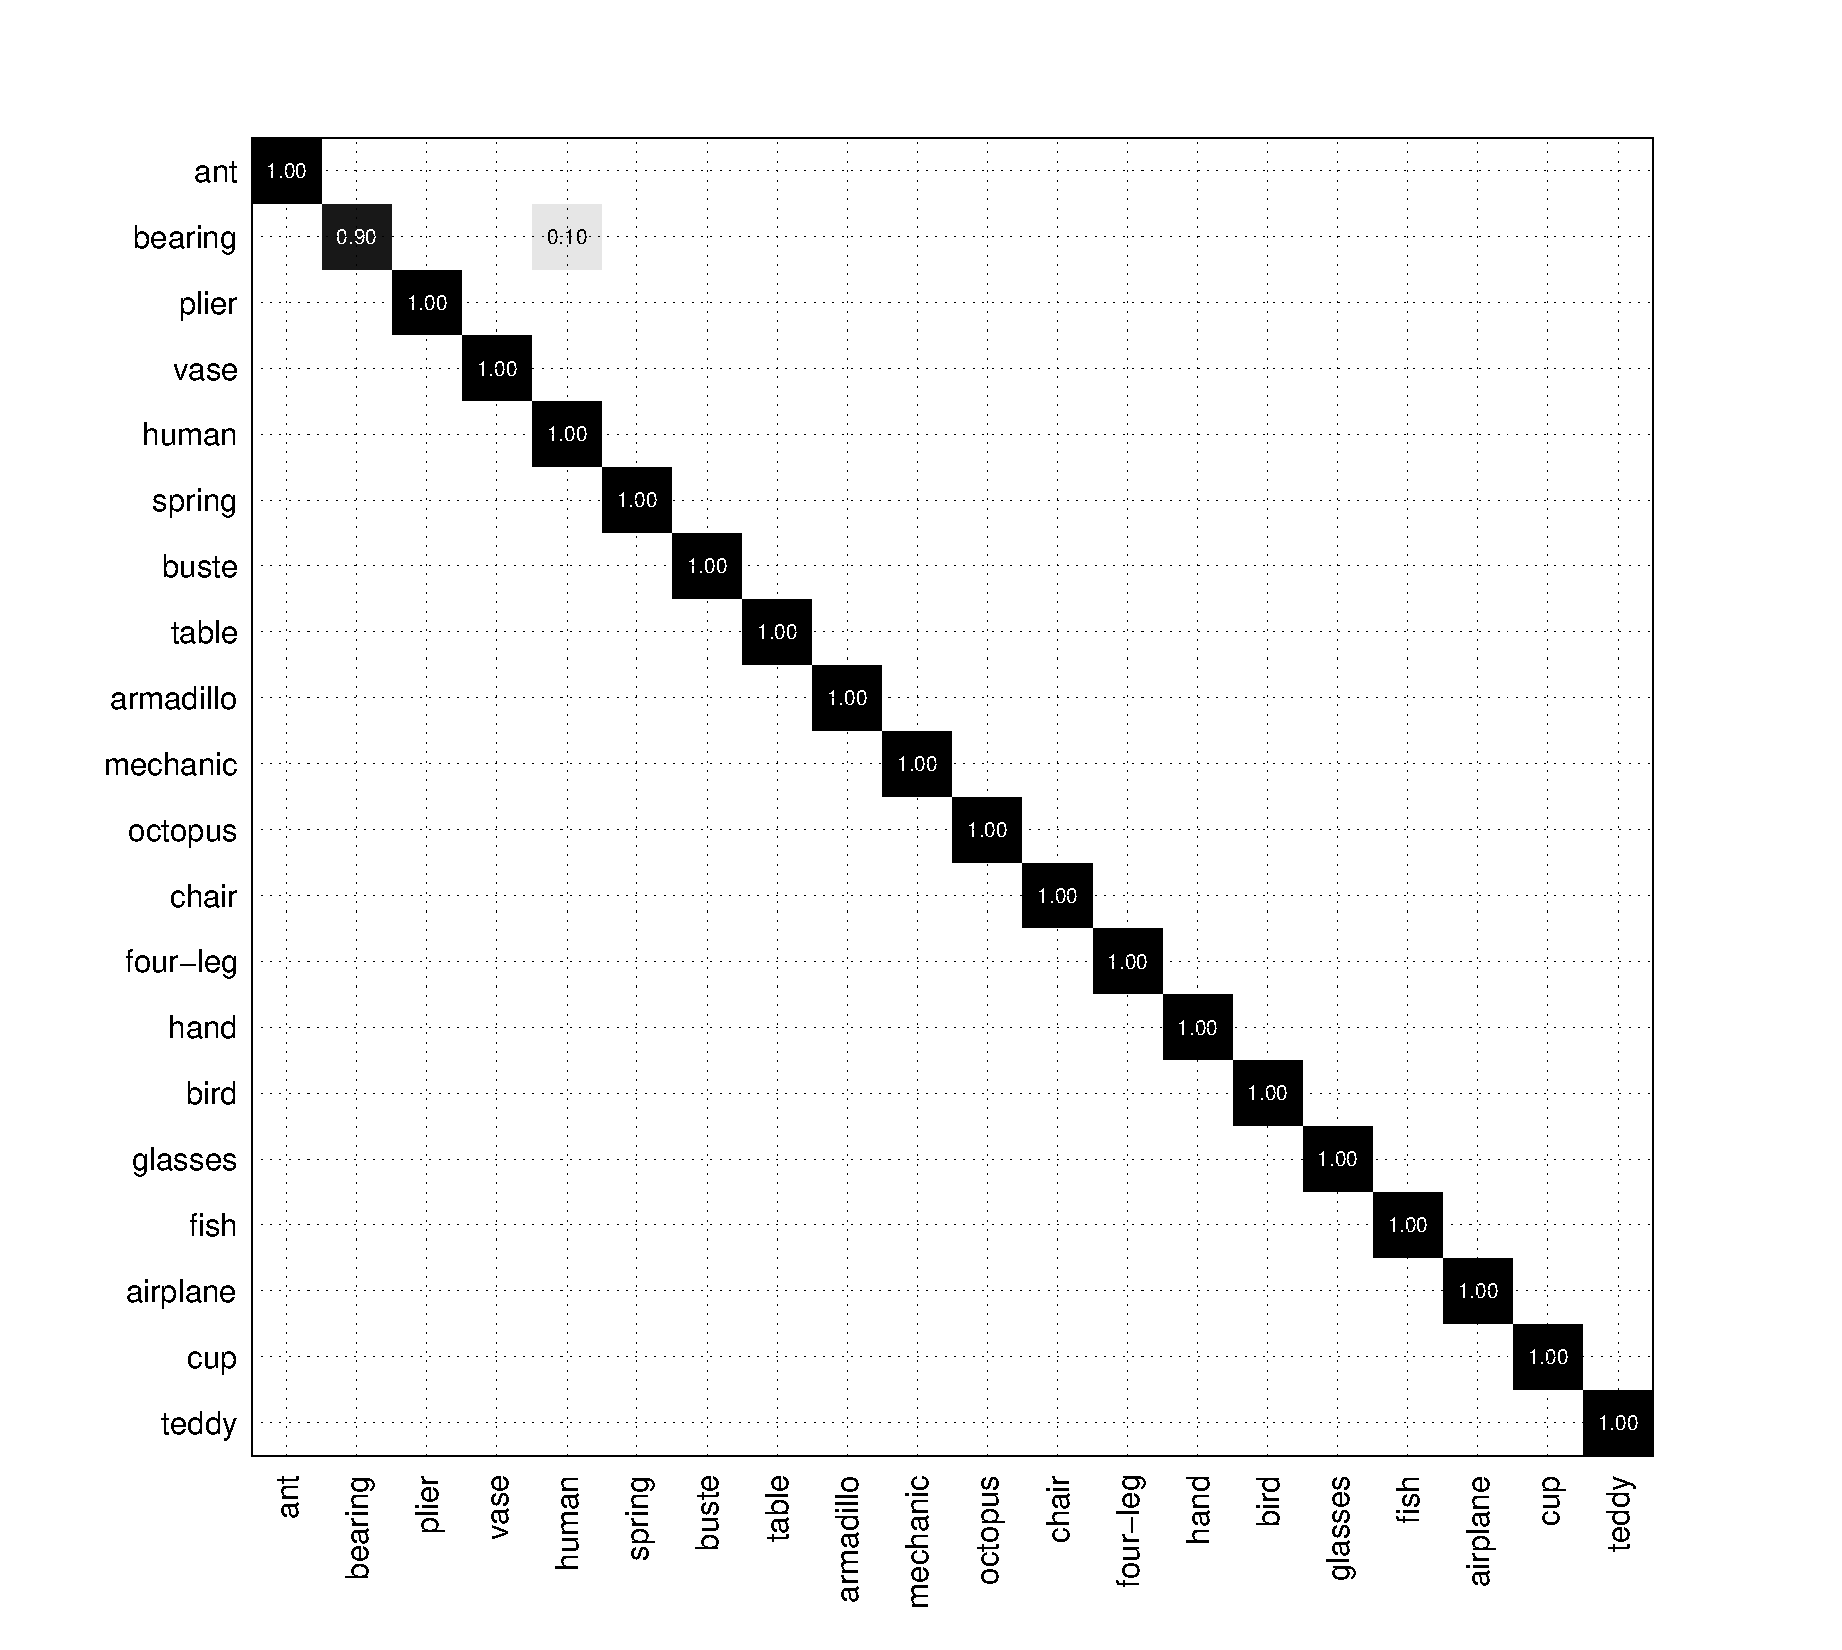
\includegraphics[width=0.98\linewidth]{figures/CM2007} 
\end{center} 
\vspace{-4mm}
\caption{在SHREC 2007上用提出的方法计算混淆矩阵。.} \label{fig_cm_shrec2007}
\end{figure*}

\begin{table}[hptb]
\caption{提出的方法的平均分类结果(\%)}\label{table_classification_results_3}
\centering
\begin{tabular}{lccc}  % {lccc} c
\hline \hline
特征                 &SHREC 2007     &SHREC 2011         & McGill \\ 
\hline
几何特征   &82.00          &70.00              & 81.69    \\ 
视觉特征       &89.22          &73.75              & 85.22\\  

3D MMF                  &\textbf{99.50} &\textbf{95.40}     &\textbf{97.47}\\  
\hline  \hline       
\end{tabular}

\end{table}

\begin{figure*}[hptb]
\begin{center}
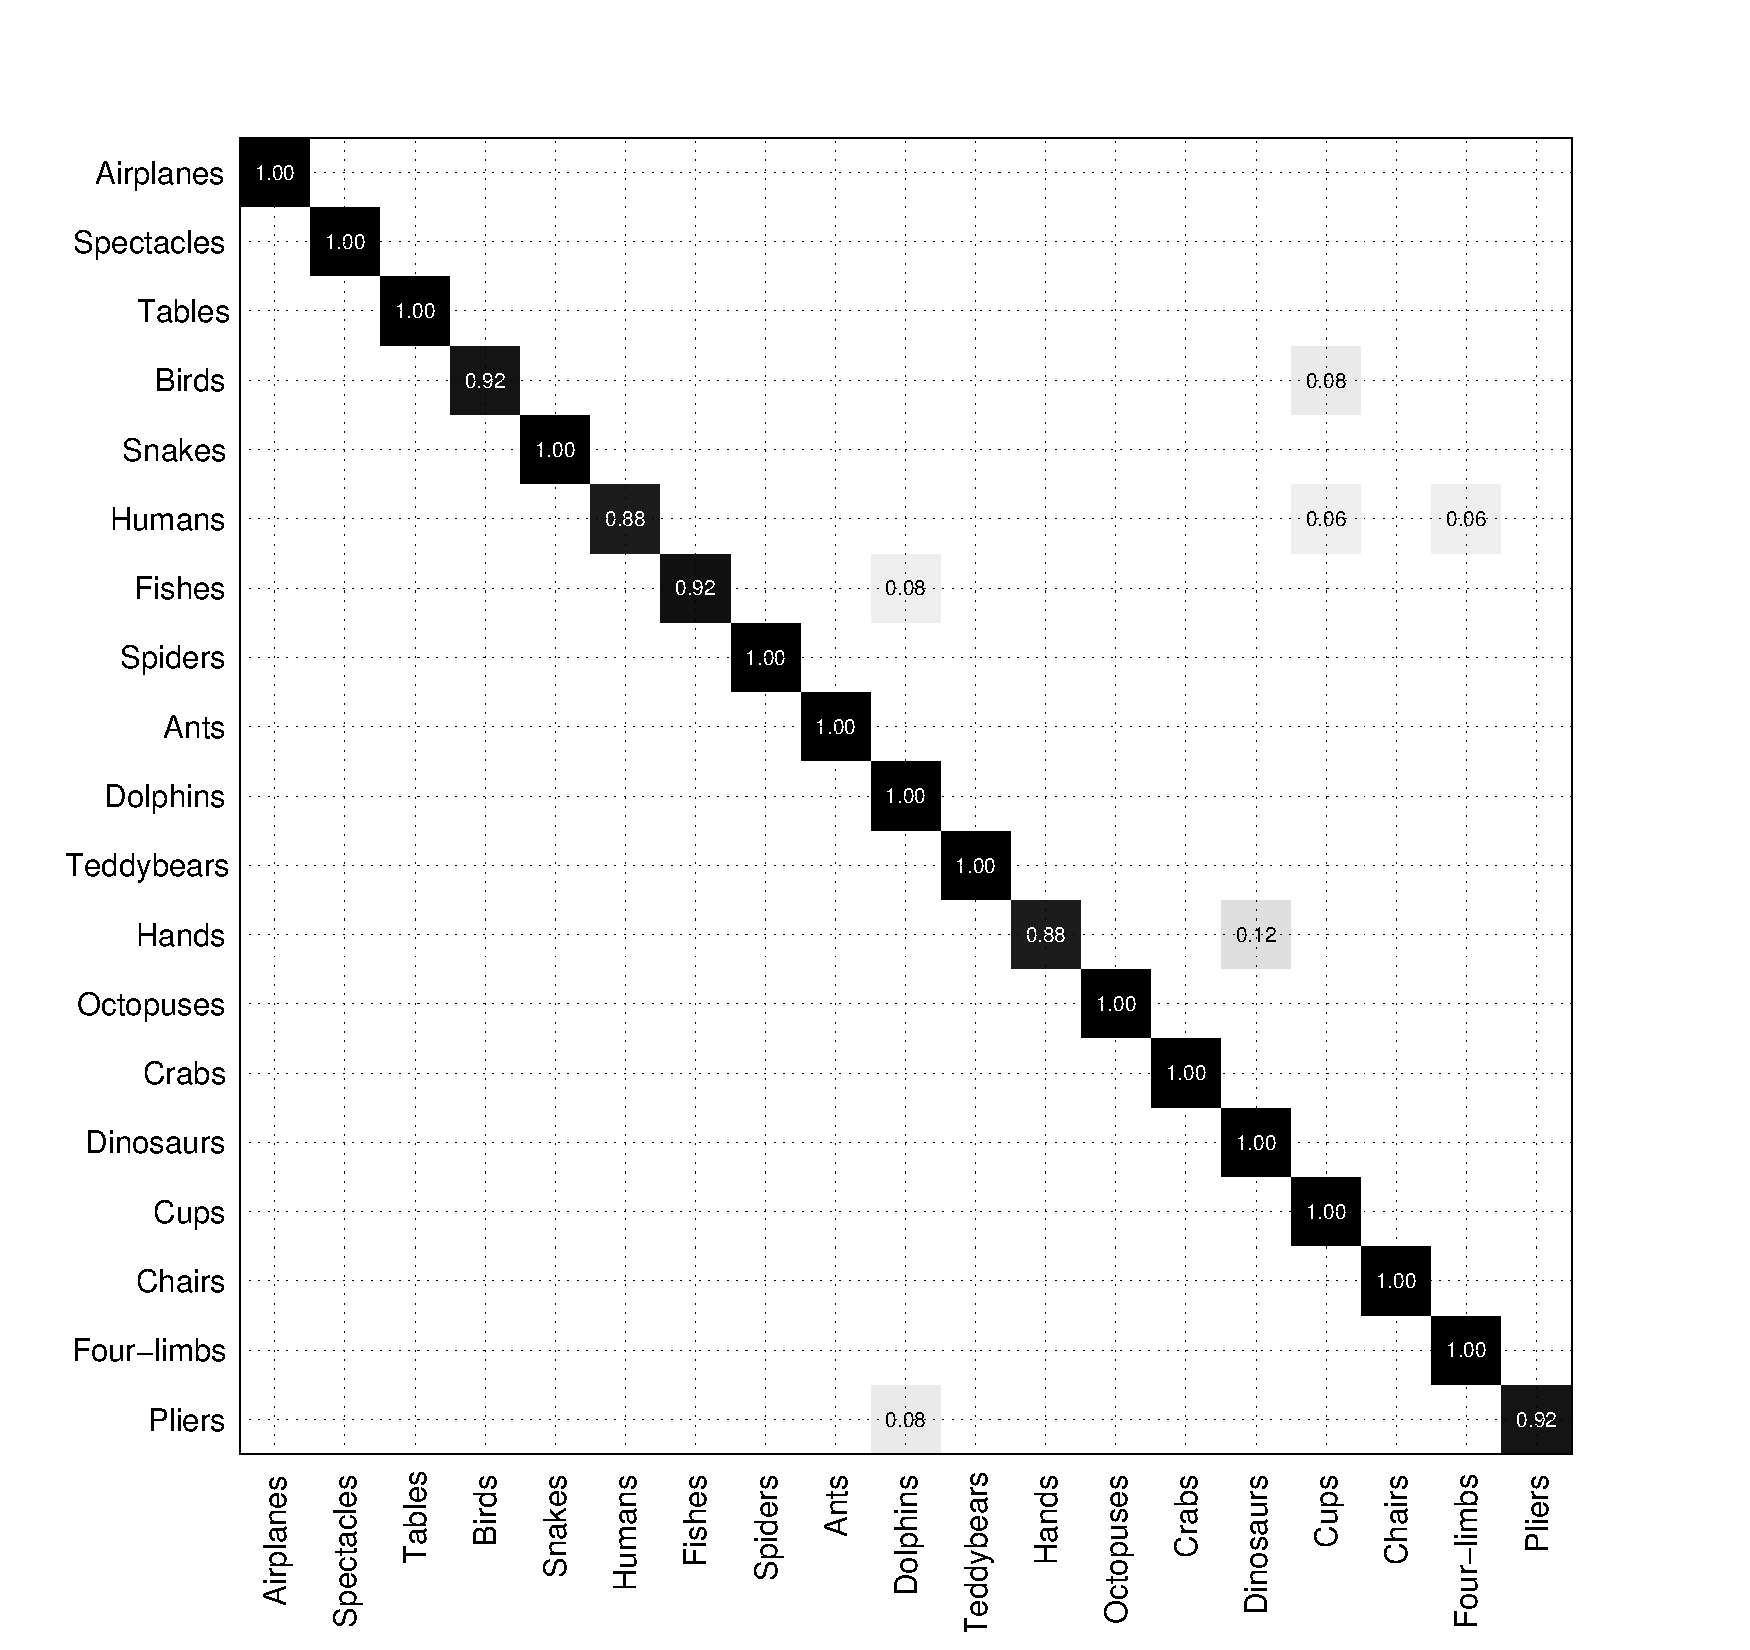
\includegraphics[width=0.98\linewidth]{figures/CMmcgill}
\end{center} 
\vspace{-4mm}
\caption{在McGill上用提出的方法计算混淆矩阵。} \label{fig_cm_mcgill}
\end{figure*}

我们分别在SHREC 2007,SHREC 2011和McGill数据集上进行分类实验,分别具有视觉描述符,几何描述符描述符和三维MMF三种类型的特征。 在表\ref {table_classification_results_3}中可以看到每个类型特征的平均分类精度。从表\ref {table_classification_results_3}中,我们可以清楚地得出结论,与仅使用单一模态特征所获得的结果相比,3D MMF实现了更好的分类性能。 这可以由几何和基于视图的模态只反映3D模型的部分属性这一事实来解释,因此,当考虑到两种不同的模态时,我们可以获得更多的判别力。 在三个数据集中,SHREC 2011的结果由于小的形状变化导致不敏感的描述,所以在SHREC 2011上的结果具有最低的准确性。 从表格中我们注意到几何描述符描述符的分类性能比视觉描述符差。 主要原因在于体素化操作像拓扑关系一样丢失了某些信息,导致性能不足,尽管体素化很容易用于CDBN模型的三维形状分析。
\begin{figure*}[hptb]
\begin{center}
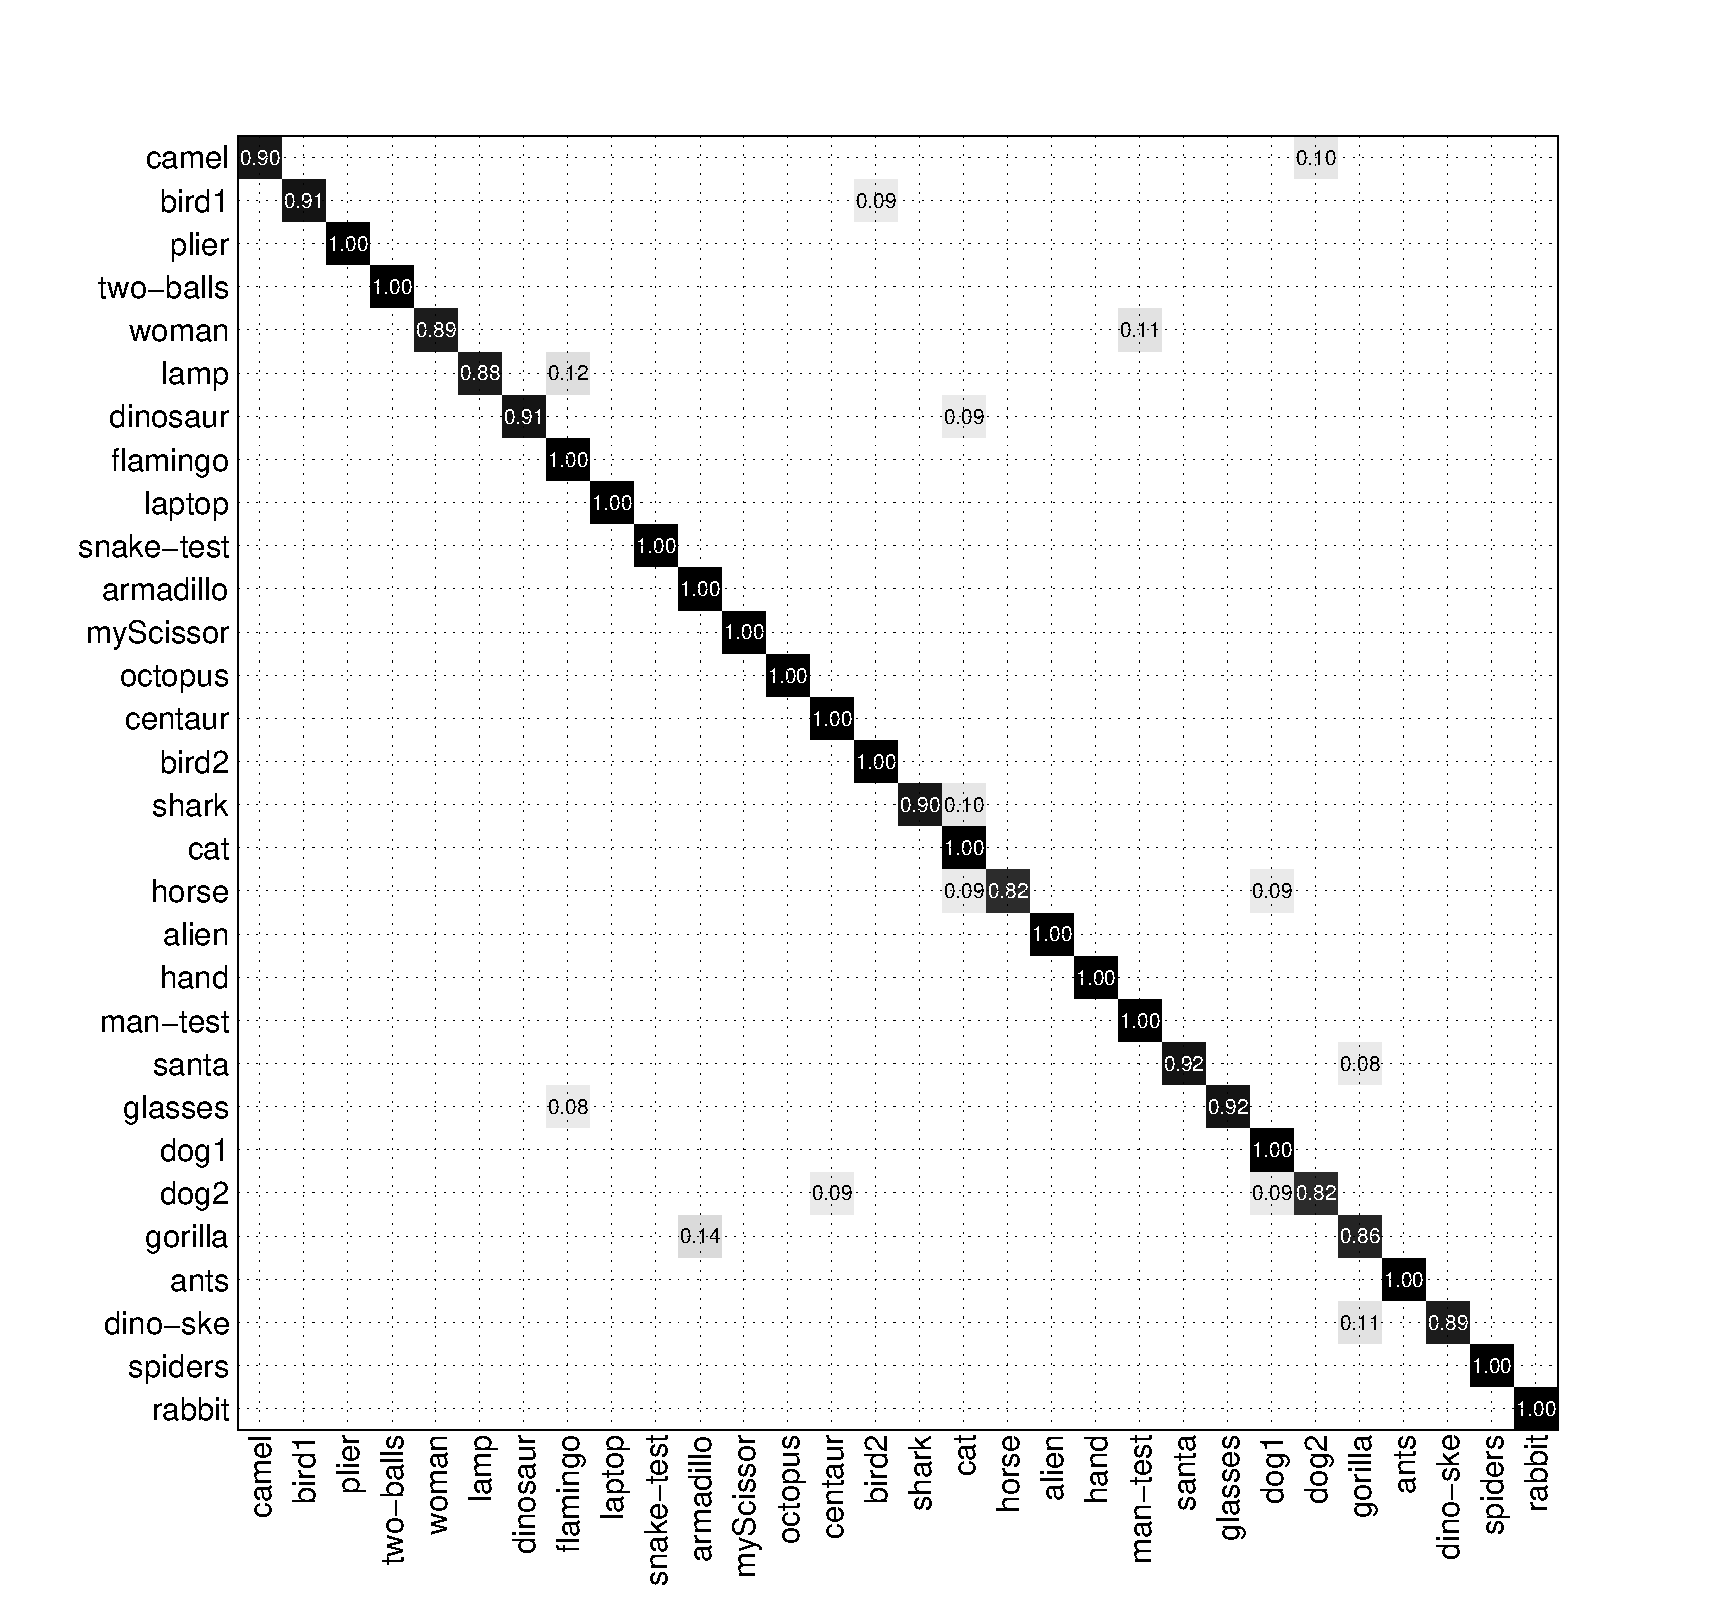
\includegraphics[width=0.98\linewidth]{figures/CM2011}
\end{center} 
\vspace{-4mm}
\caption{在SHREC 2011上用提出的方法计算混淆矩阵。} \label{fig_cm_shrec2011}
\end{figure*}


在机器学习领域,混淆矩阵是一种特定的表格布局,允许可视化算法的性能。 混淆矩阵包含有关分类系统完成的实际分类和预测分类的信息。 不同的颜色提供不同的概率。 为了进一步详细分析识别结果,在三维数据集上对三维数据集进行分类的混淆矩阵在图\ref {fig_cm_shrec2007}, \ref{fig_cm_mcgill}和\ref {fig_cm_shrec2011}可见。 从结果中可以得出结论,所提出的方法在SHREC2007、SHREC2011和McGill数据集的错误分类很低,之所以在SHREC2011上的表现相对于其他数据集稍微有点差,是因为SHREC2011数据集中包含许多十分相似的模型,不同的三维模型类间差距不大,因此实际上增加了分类的难度,但最终也取得了较好的结果,说明该方法具有广阔的应用前景。

\subsection{检索实验}

\begin{figure}[tbhp]
\begin{center}
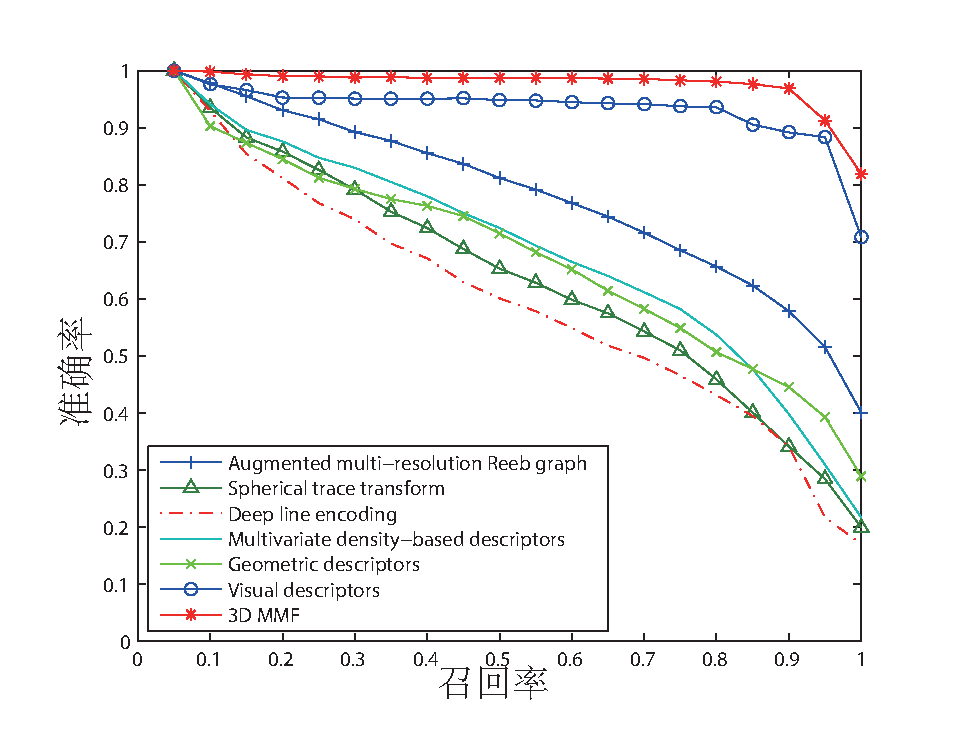
\includegraphics[width=1\linewidth]{figures/PR2007}
\end{center} 
\vspace{-4mm}
\caption{一些最先进的方法和提出的方法在SHREC 2007的PR曲线.} \label{fig_rp_shrec2007}
\end{figure}

对于检索任务,有6个标准评估指标用于评估推荐方法的性能。 它们是 precision-recall curve, nearest neighbor (NN), first tier (FT), second tier (ST), E-measure (E), 和 discounted cumulative gain (DCG),详细的定义可以在\cite{shilane2004princeton}中找到。 我们使用在分类实验中训练的模型来计算每个3D形状的3D MMF。 等式 \eqref{cal_cal_distance}被用来描述两个模型之间的相似性。

%table
\begin{table}[tbhp]

\caption{SHREC 2007上的20,40,60和80个返回项目的精度值(\%)} \label{table_retrieval_shrec2007_precision}
\begin{center}
\begin{tabular}{cccccc}  % {lccc} 表示各列元素对齐方式,left-l,right-r,center-c
\hline  \hline
方法 			    &20     &40     &60     &80   \\ 
\hline
DLE \cite{giorgi2007watertight}   &54.6  &32.9  &24.1  &19.0   \\ 
MDD \cite{giorgi2007watertight}      &62.6  &36.6  &26.2  &20.5  \\
STT \cite{giorgi2007watertight}      &56.4  &34.6  &25.2  &19.9  \\
SI-MSC \cite{giorgi2007watertight}      &60.4  &36.6  &26.2  &20.5  \\
aMRG \cite{giorgi2007watertight}      &71.4  &41.4  &29.0  &22.5  \\
ERG \cite{barra20133d}      &62.4  &41.5  &30.5  &24.4  \\
3D MMF   &\textbf{97.2} &\textbf{49.4} &\textbf{33.0} &\textbf{24.8} \\  
\hline  \hline      % & 表示列的分隔线 
\end{tabular}
\end{center} 
\end{table}


\textbf{在SHREC 2007上的检索实验。} 我们在SHREC 2007数据集上进行检索实验来评估检索性能。我们的方法和一些最先进的方法的召回精度曲线如图\ref{fig_rp_shrec2007}所示,其中包括深度线编码(DLE)\cite{Giorgi2008SHape},多元密度描述符(MDD)\cite{Giorgi2008SHape},球面轨迹变换(STT)\cite{Giorgi2008SHape},轮廓交点和多尺度轮廓(SI-MSC)\cite{Giorgi2008SHape},增强的多分辨率Reeb图(aMRG)\cite{Giorgi2008SHape}和扩展的Reeb图(ERG)\cite{barra20133d}。数据集中所有模型的平均精度和召回率的数值分别列于表\ref {table_retrieval_shrec2007_precision}和\ref{table_retrieval_shrec2007_recall}中。我们列出了返回的20,40,60和80项的值,它们是每个类的大小的1,2,3和4倍。从图和表中可以清楚地看出,提出的方法达到最佳整体检索结果。检索实验采用来自体素的几何描述符和来自视图的视觉描述符。虽然只有视觉特征的表现明显优于竞争对手,但3D MMF仍然比它好。原因在于单一特征只能提供三维形状的特定方面信息,而所提出的方法则是基于形状和视图的形式信息融合。因此,3D MMF包含3D模型的内在属性和外在属性。同时3D MMF增加了类内相似度,降低了类间相似度。结果,检索性能得到改善。

%table
\begin{table}[tbhp]

\caption{SHREC 2007上的20,40,60和80个返回项目的召回率(\%)} \label{table_retrieval_shrec2007_recall}
\begin{center}
\begin{tabular}{cccccc}  % {lccc} 表示各列元素对齐方式,left-l,right-r,center-c
\hline  \hline
方法 			    &20     &40     &60     &80   \\ 
\hline
DLE \cite{giorgi2007watertight}   &54.6  &65.8  &72.4  &76.3   \\ 
MDD \cite{giorgi2007watertight}      &62.6  &73.2  &78.6  &82.1  \\
STT \cite{giorgi2007watertight}      &56.4  &69.2  &75.6  &79.8  \\
SI-MSC \cite{giorgi2007watertight}      &60.4  &73.2  &78.8  &82.2  \\
aMRG \cite{giorgi2007watertight}      &71.4  &82.8  &87.2  &90.2  \\
ERG \cite{barra20133d}      &62.4  &82.9  &91.6  &97.5  \\
3D MMF   &\textbf{97.2} &\textbf{98.8} &\textbf{99.1} &\textbf{99.3} \\  
\hline  \hline      % & 表示列的分隔线 
\end{tabular}
\end{center} 
\end{table}

%table
\begin{table}[tbhp]
\caption{在SHREC 2007上使用标准测量方法检测提出的方法的检索性能(\%)} \label{table_retrieval_shrec2007}
\begin{center}
\begin{tabular}{cccccc}  % {lccc} 表示各列元素对齐方式,left-l,right-r,center-c
\hline  \hline
特征 			    &NN     &FT     &ST     &E      &DCG \\ 
\hline
几何特征   &85.50  &57.82  &36.11  &50.70  &86.78 \\ 
视觉特征      &96.50  &86.98  &47.99  &68.61  &97.26 \\
3D MMF                  &\textbf{99.75} &\textbf{91.77} &\textbf{49.07} &\textbf{71.43} &\textbf{99.16}\\  
\hline  \hline      % & 表示列的分隔线 
\end{tabular}
\end{center} 
\end{table}


\begin{figure}[tbhp]
\begin{center}
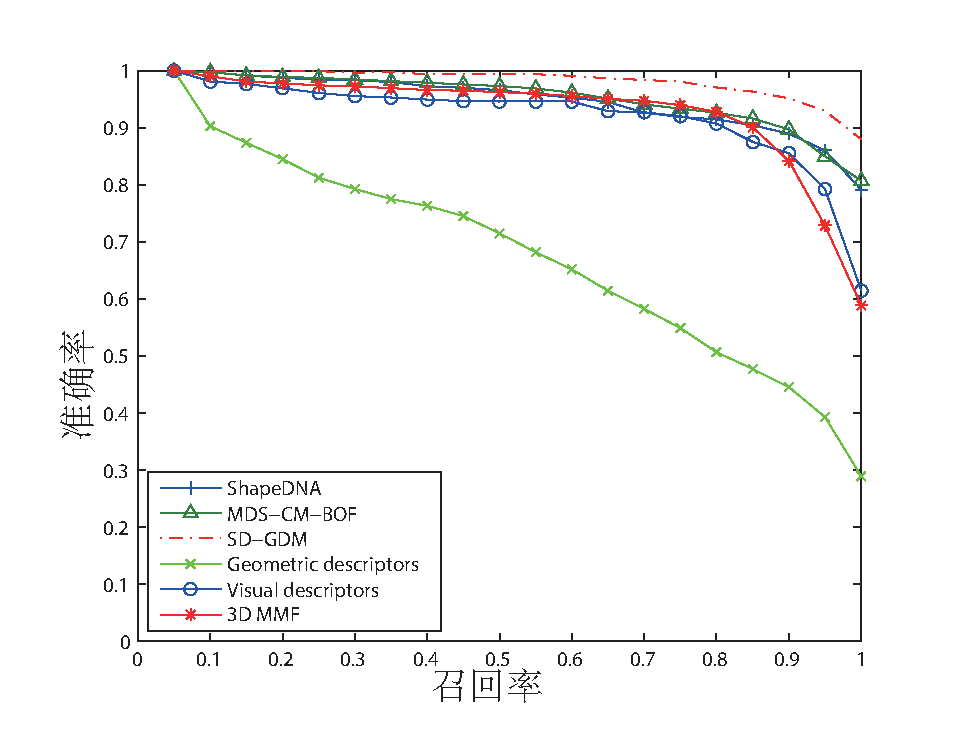
\includegraphics[width=1.0\linewidth]{figures/PR2011}
\end{center} 
\vspace{-4mm}
\caption{一些最先进的方法和提出的方法在SHREC 2011的PR曲线} \label{fig_rp_shrec2011}
\end{figure}

\begin{figure}[tbhp]
\begin{center}
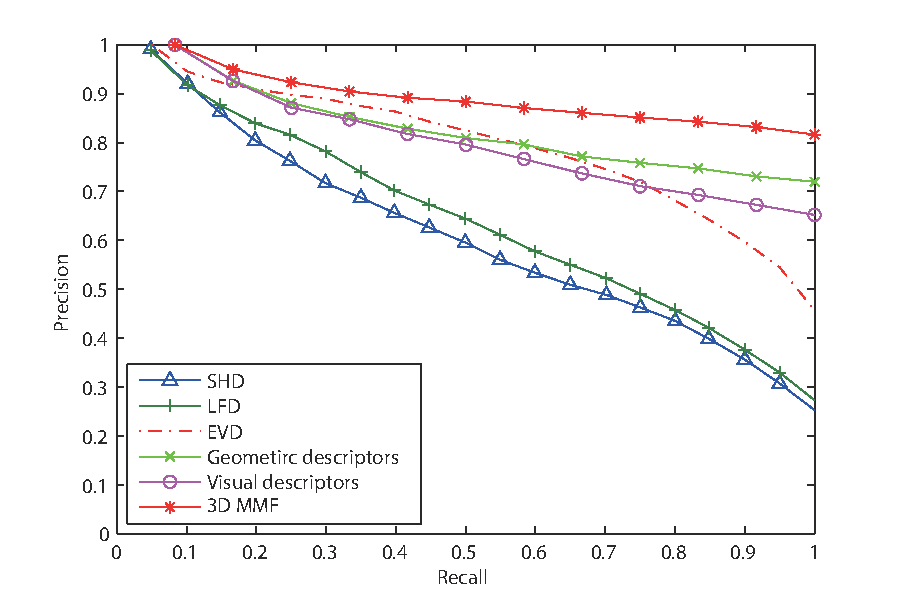
\includegraphics[width=1.0\linewidth]{figures/Mcgill_PR}
\end{center} 
\vspace{-4mm}
\caption{一些最先进的方法和提出的方法在McGill的PR曲线} \label{fig_rp_McGill}
\end{figure}

表\ref {table_retrieval_shrec2007}列出了数字评估结果。 从表格中我们可以清楚地看到,所有的措施都从使用单一模式特征到多模态特征得到了很大的改善。 NN,FT,ST,E,DCG指数的平均改善程度分别为8.75%,19.37%,7.02%,11.78%,7.14%,说明多模式融合法产生的三维MMF具有 提高检索性能的出色能力。




\textbf{SHREC 2011和McGill的检索实验。}
我们还对SHREC 2011和McGill数据集进行检索实验,以评估检索性能。 我们的方法和一些最先进的方法的召回精度曲线绘制在图\ref {fig_rp_shrec2011}和\ref {fig_rp_McGill}。 表\ref {table_retrieval_results_shrec2011}和\ref {table_retrieval_results_McGill}列出数字评估。 结果表明,该方法的检索性能具有广阔的应用前景。

%table
\begin{table}[tbhp]
\caption{在SHREC 2011上使用标准测量方法检测提出的方法的检索性能(\%)} \label{table_retrieval_results_shrec2011}
\begin{center}
\begin{tabular}{cccccc}  % {lccc} 表示各列元素对齐方式,left-l,right-r,center-c
\hline  \hline
特征                 &NN &FT &ST &E &DCG\\ 
\hline
几何特征  &85.50 &57.81 &36.11 &50.70 &86.78   \\ 
视觉特征     &96.83 &86.02 &46.51 &\textbf{89.39} &96.86\\                   
3D MMF              &\textbf{98.00} &\textbf{86.85} &\textbf{46.80} &67.76 &\textbf{97.35}\\  
\hline  \hline      % & 表示列的分隔线 
\end{tabular}
\end{center} 
\end{table}



%table
\begin{table}[tbhp]

\caption{在McGill上使用标准测量方法检测提出的方法的检索性能(\%)}\label{table_retrieval_results_McGill}
\begin{center}
\begin{tabular}{cccccc}  % {lccc} 表示各列元素对齐方式,left-l,right-r,center-c
\hline  \hline
特征                 &NN &FT &ST &E &DCG\\ 
\hline
几何特征   &88.84 &62.45 &37.68 &59.66 &88.37    \\ 
视觉特征      &87.30 &54.12 &36.23 &51.91 &86.51\\                   
3D MMF              &\textbf{92.12} &\textbf{73.19} &\textbf{42.12} &\textbf{68.55} &\textbf{92.38}\\  
\hline  \hline      % & 表示列的分隔线 
\end{tabular}
\end{center} 
\end{table}

\section{总结}
本节提出了一种新的三维形状识别与检索的多模态特征提取与融合方法。 首先,通过CDBN和CNN分别提取几何描述符和视觉描述符作为基于几何的特征和基于视图的特征。 然后采用两个DBN学习结构化的高层描述符。 此外,为了发现模式之间的深层相互关系,我们利用RBM来融合这些高级特征。 在分类和检索任务的标准基准上进行的实验已经证明,与最先进的方法相比,所提出的方法实现更好的性能。 实验结果表明,融合表示具有较强的判别能力,能够抑制类内变异,增强类间相似性分离。

与传统的计算机视觉形态分析方法不同,我们充分考虑了内在属性和外在视觉相似性。 另外,我们不是简单地融合几何和视觉特征来训练模型,相反,我们采取的策略是首先通过DBN学习高级特征,通过DBN去除特定于模态的信息,然后是高层特征融合学习形状分析的多模态特征。 通过使用这种策略,可以对基于几何的模型和基于视图的模态之间高度非线性的相关性进行全面建模。

\textbf{局限性。} 在生成几何描述符的过程中,网格尺寸越小,精度越高,但计算量呈指数增长。 因此,应该设计一个合适的方法来平衡这两个方面。在我们的框架下,为了学习三维形状的融合表示,我们将不同模式的高层特征连接起来。 然而,每个形态特征携带的信息并不完全相同,从SHREC 2007数据集上的实验可以看出,视觉描述符比几何描述符包含更多的信息。 因此,应寻求解决办法来表示不同形式的重要性。 此外,在所提出的方法中,深度学习的特征是全局性的,使得三维形状的局部信息或多或少地丢失。 因此,该方法难以应用于更复杂的任务,如分割,局部检索和对称检测。

\textbf {未来的工作。} 首先,目前我们只研究框架中的几何和视觉描述符。 为了更好地描述三维形状,我们将探索将各种形式的全局特征和局部特征相结合的可能性。 其次,研究其他方法可以保留更多的结构信息进行特征学习。第三,研究可以直接处理图形数据的深度学习方法,包括三维网格数据,communication network和traffic network,这将会引起其更广泛的应用和更好的性能。



% 第四章 

\chapter{用有限信息进行三维形状识别的深度时空网络}

在过去几年的相关工作创造性地提出了一些基于深度学习的三维形状描述符,它们具有很强的学习高层次特征的能力,但其中大部分只是使用深度学习方法来提取高层特征,而忽略获取信息的时空关系。以至于捕获的视图分别被训练和使用。为了使三维形状识别与检索系统适用于移动机器人与环境的自主交互,需要使用模仿人的空间相关图像来实现高精度的物体识别。在本文中,我们提出了一种新的三维形状识别和检索框架,它通过记忆机制同时学习高级特征和对时空信息进行建模。本文提出了一种新颖的三维形状识别与检索框架,结合卷积神经网络(CNNs)和长短期记忆(LSTM),学习了三维物体视觉信息的时空序列关系。具体而言, CNNs是“视觉系统”,因为它具有强大的提取有效视觉特征的能力,而LSTM是“记忆系统”,因为该模型可以学习不同视觉特征的时空顺序关系。大量的实验表明,所提出的框架对使用有限的序列信息能够获得较好的性能。

虽然前面提到的几何,视觉和深度学习三种方法在计算机图形学界已经做出了很大的贡献,但是对于在真实环境中识别三维物体的移动机器人来说,还远远不能令人满意。 首先,移动机器人应该以较少的视角做出快速准确的判断,这就要求视角特征的高质量。其次,大多数现有的形状描述符忽略了连续帧探测的信息。 这两个问题限制了机器人在真实复杂的世界中实现自由操作。 综合考虑,本文提出了一个新的框架,它包含两个过程,即基于视图的描述符生成和基于记忆的时空信息建模。

\begin{figure*}[tbh]
\begin{center}
 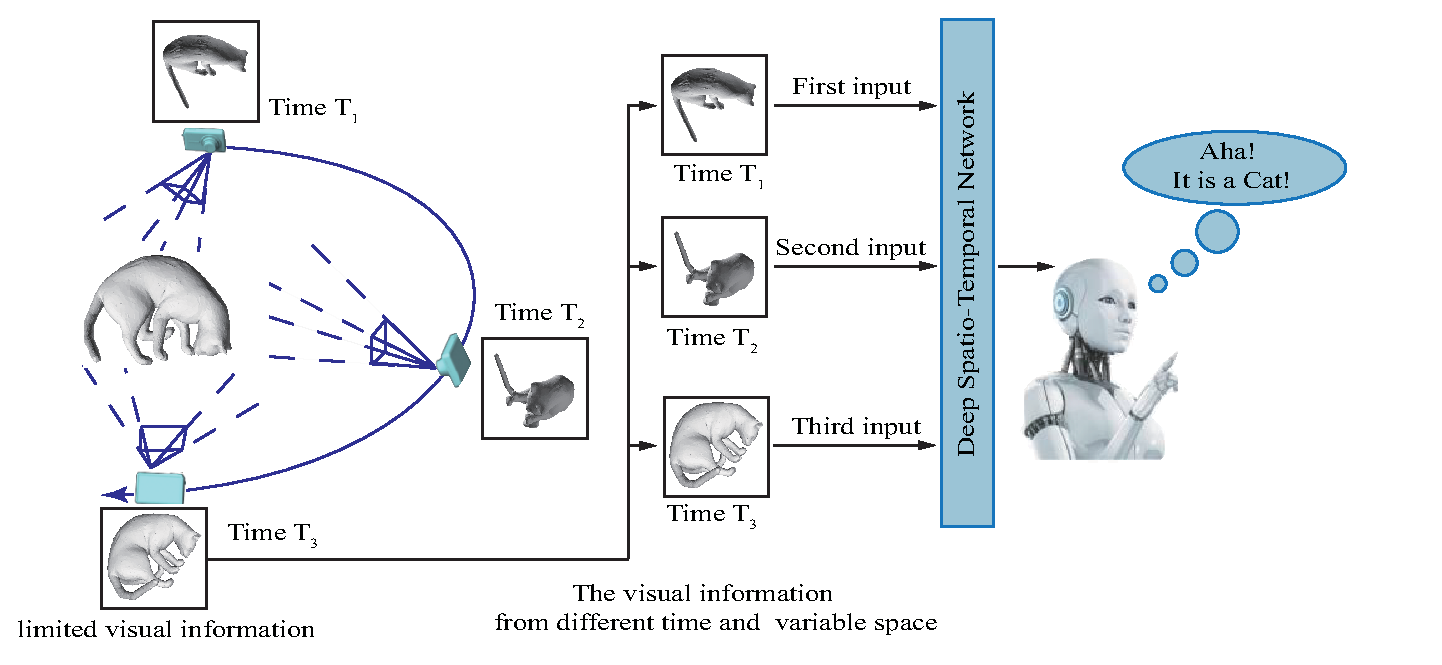
\includegraphics[width=0.98\linewidth]{figures/flowchart.eps}
 \end{center} \vspace{-4mm}
\caption{三维形状的深度时空网络} 
\label{flowchart4}
\end{figure*}

本节提出的方法流程图如图\ref{flowchart4}所示,展示了CNN和LSTM生成的深层时空特征的框架。 在生成二维投影的过程中,由于深度相机以一定的顺序拍照,投影包含一定的时空序列关系。在视觉特征提取中,我们以深度图像为输入,不需要下采样。为了探索二维图像的时空顺序关系,我们的方法是利用LSTM模型的顺序数据学习能力。我们引导LSTM具有监督学习结构,学习的三维形状表示。每一步的细节如下。

\section{所涉及的深度学习方法介绍}
\textbf{长短期记忆网络(LSTM)}
中文分词、词性标注、命名实体识别、机器翻译、语音识别都属于序列挖掘的范畴。序列挖掘的特点就是某一步的输出不仅依赖于这一步的输入,还依赖于其他步的输入或输出。在序列挖掘领域传统的机器学习方法有HMM(Hidden Markov Model,隐马尔可夫模型)和CRF(Conditional Random Field,条件随机场),近年来又开始流行深度学习算法RNN(Recurrent Neural Networks,循环神经网络)。

\textbf{循环神经网络 (RNN)}

CNN等传统神经网络的局限在于:将固定大小的向量作为输入(比如一张图片),然后输出一个固定大小的向量(比如不同分类的概率)。不仅如此,CNN还按照固定的计算步骤(比如模型中层的数量)来实现这样的输入输出。这样的神经网络没有持久性:假设你希望对电影中每一帧的事件类型进行分类,传统的神经网络就没有办法使用电影中先前的事件推断后续的事件。
RNN 是包含循环的网络,可以把信息从上一步传递到下一步。

RNN的循环展开之后其实就是同一个网络复制多份,次序连接进行信息传递。RNN允许信息的持久化,对当前的状态保留记忆(以隐变量的方式存在,也就是图中计算$h_{t}$需要用到$h_{t-1}$的信息)。对于同一个RNN来说,其“A结构”(绿色部分)是固定的(共享一套参数,毕竟是从循环展开来的啊肯定是一样的)。

\textbf{RNN弊端和LSTM}
RNN 是在有顺序的数据上进行学习的. 为了记住这些数据, RNN 会像人一样产生对先前发生事件的记忆。 在反向传递得到的误差的时候, 他在每一步都会 乘以一个自己的参数 W。如果这个 W 是一个小于1 的数, 比如0.9. 这个0.9 不断乘以误差, 误差传到初始时间点也会是一个接近于零的数, 所以对于初始时刻, 误差相当于就消失了。 我们把这个问题叫做梯度消失或者梯度弥散 Gradient vanishing. 反之如果 W 是一个大于1 的数, 比如1.1 不断累乘, 则到最后变成了无穷大的数, RNN被这无穷大的数撑死了, 这种情况我们叫做剃度爆炸, Gradient exploding. 这就是普通 RNN 没有办法回忆起久远记忆的原因.

因为RNN的信息只能传递给相邻的后继者(从循环展开之后的表示来看),因此当输出与其相关的输入信息相隔较近的时候,普通的RNN是可以胜任的。而当这个间隔很长的时候,虽然理论上RNN是可以处理这种长期依赖 (Long Dependencies) 的问题,但是实践中并没有成功。Bengio, et al. (1994)等人对该问题进行了深入的研究,他们发现了使训练 RNN 变得非常困难的根本原因(梯度消失/梯度爆炸)。相关信息输入与需要该信息的输出之间间隔很长。因此,Hochreiter和Schmidhuber (1997)提出了Long Short Term Memory 网络 (LSTM),并在近期被Alex Graves进行了改良和推广。



\section{CNN提取视觉描述符}

从视角来分析3D形状的流行方式是将3D模型从各个角度转换成2D图像。 理论上,这些二维图像应尽可能包含来自三维模型的信息。 在我们的视觉描述符生成过程中,我们首先将三维形状投影到二维图像中,并采用CNN进一步提取视觉特征。 我们的算法的细节总结如下。

\textbf {3D模型预处理。} 在这部分中,我们将原点设置在三维模型质心的中心,然后测量点的最大极距到其表面上的一个点。 虽然没有旋转归一化,但是这将在后面一定程度上被补偿。

\textbf{深度图像的采集。} 深度图像,一种二维图像,来自于从质心居中的正十二面体的20个顶点的虚拟相机的拍摄。在所提出的方法中,我们旋转正十二面体10次以使该特征对旋转具有鲁棒性。应该仔细设置旋转角度,以确保所有相机均匀分布,并能够覆盖3D模型的不同视角。 我们认为十二面体有20个顶点可以产生中等数据量,从而保证高计算性能和重要的信息。 该策略与LFD在视图提取方面类似,但略有不同,我们丢弃二值图像,只使用二维深度图像。 最后一个3D模型由200个图像表示,每个图像的大小为256×256。
\begin{figure*}[tbhp]
\begin{center}
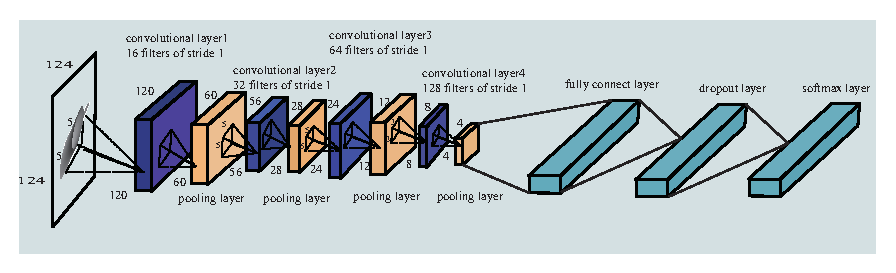
\includegraphics[width=0.9\linewidth]{figures/CNN_LSTM_view.eps}
\end{center} 
\vspace{-4mm}
\caption{我们的3D形状CNN模型的结构。为了说明的目的,我们只为每个卷积层绘制一个滤波器。 从单个视图中提取视觉特征,CNN有着完美的表现。} \label{fig_CNN_view}
\end{figure*}
在深度图像渲染中,有效信息集中在图像的中心。 因此,我们移除深度图像的边界,并将图像从256×256裁剪成124×124的大小,以滤除干扰和冗余信息,从而使数据紧凑。 另外,由于图像尺寸小于原始深度图像,该处理可以促进之后的CNN特征学习。 因为CNN模型的有效输入范围是从0到1,所以深度图不适合作为CNN模型的输入。 因此,我们将每个维度的范围标准化为[0,1]。



\textbf {视觉描述符。} CNN是一种功能强大的深度学习技术,在计算机视觉领域取得了很好的图像特征提取。从上面的程序中,我们获得包含丰富的关于3D模型的视觉信息的2D图像。因此,CNN被用来提取3D形状的每个图像的视觉特征。如图\ref{fig_CNN_view}所示,CNN由4个卷积层组成,其后是一个完全连接层,一个dropout层和一个softmax分类层用于提取二维图像的特征。对于每个卷积层$ l $,我们有:
%
\begin{equation}
	\mathbf{F}_l = pool(ReLU(\mathbf{W}_l * \mathbf{F}_{l-1} + \mathbf{b}_l)),
\label{cal_CNN}
\end{equation}
%
其中$ l\in \{1,...,4 \} $,$ \mathbf {b} _l$是$ l $ -th层的偏置参数,$ \mathbf {W} _l $是卷积核。初始特征图是2D图像$ \mathbf {F}_0 $。整流线性单位(ReLU)激活函数是阈值函数,当变量小于0时为零,然后当变量大于0时与斜率1呈线性关系。池操作是考虑激活的邻域并在每个激活中产生激活函数。 Max-pooling算子是该作品池函数,它在邻域内得到最大的数值被激活,并给平移带来内置的不变性。CNN网络由四个卷积层组成。滤波器的数目从1 $ st $到最后一个卷积层设置为16,32,64,128,所有图层的滤波器大小分别设置为5,5,5,3。所有pooling层大小设置为2.在网络末端增加了dropout层,以避免过度拟合。在这个框架下,我们使用反向传播方法,输入为3D形状的深度图像和相应的标签。在完成CNN模型训练之后,对于每个输入深度图像,使用CNN的正向公式生成相应的视觉描述符$o(\mathbf{X}_{2D})$。

一般来说,视觉描述符对于三维形状识别任务是不够的,因为三维形状只从一个角度不能完全表示三维形状。 作者发下视觉描述符的时空顺序关系被忽略。 因此,作者探索不同视点的时空序列关系,进一步挖掘三维模型的内在特征。

\section{LSTM提取深度时空特征}

传统的神经网络很少学习序列信息,这似乎是一个主要的缺陷。递归神经网络解决了这个问题,即网络中存在循环,并允许信息持续存在。 传统的递归神经网络通过将输入序列映射到隐藏状态以及隐藏状态通过以下等式来输出时间动态模型:
%
\begin{equation}
 h_{t} = g(W_{xh}*x_{t} + W_{hh}*h_{t-1} + b_{h}),
\end{equation}
%
\begin{equation}
 z_{t} = g(W_{hz}*h_{t} + b_{z}) .
\end{equation}
%
其中g是元素非线性,$h_t \in R^N$是包含$N$个隐藏单位的隐藏层,$ z_t $是时间$ t $的输出。 对于长度为$ T $的输入序列$ <x_1,x_2,...,x_T> $,上面的更新按$h_1$ ($h_0 = 0$),$z_1, h_2, z_2, ..., h_T, z_T$的顺序计算。 尽管RNN在语音识别和文本生成等任务中已经证明是成功的,但是要培养他们学习长期动态性还是很困难的。 LSTM提供了一个解决方案,通过结合记忆单元,明确允许网络学习何时“忘记”以前的隐藏单元,何时更新隐藏状态,给出新的信息。过程的细节如下。

\textbf {输入预处理}。 在LSTM体系结构中,序列长度根据输入数据的序列大小而变化。 在我们的框架中,我们对LSTM体系结构采用不同的序列长度来学习3D形状的多视图特征。

\begin{figure*} [htbp]
\begin{center}
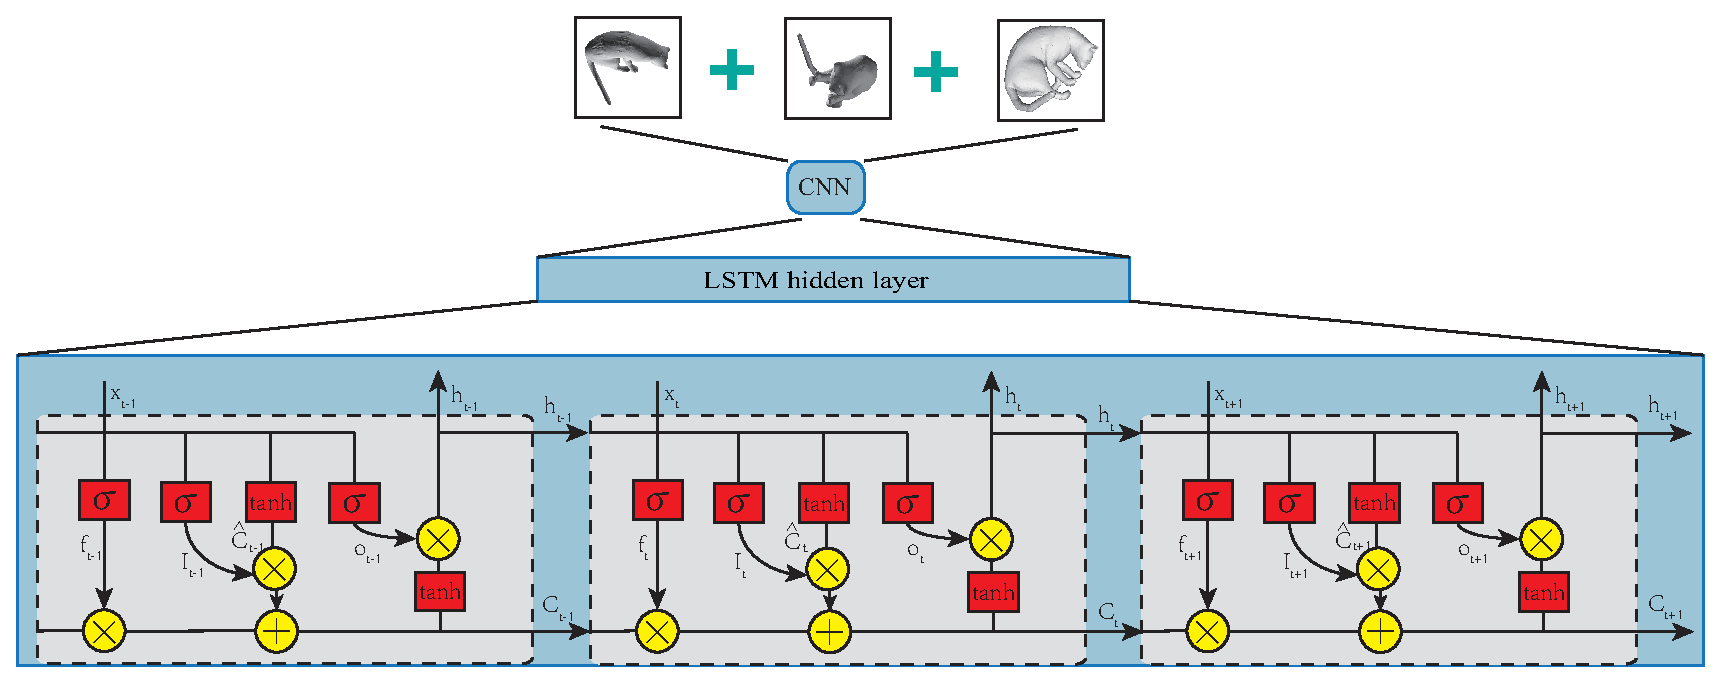
\includegraphics[width=0.98\linewidth]{figures/CNN_LSTM_lstm.eps}
\end{center} 
\vspace{-4mm}
\caption{我们的LSTM模型的体系结构。 为了说明的目的,我们只用三个多视图的三个步骤。 LSTM模型具有很强的学习三维形状学习不同视角的隐藏时空序列信息的能力。 }
\label{fig_lstm}
\end{figure*}

\textbf {时空描述符}。 随着对LSTM的研究的深入,已经提出了在记忆单元内多个不同连接的隐藏单元。 我们使用LSTM单元如下。 如图\ref{fig_lstm}所示,LSTM的存储单元包含四个主要部分,包括输入门,自回归神经元,忘记门和输出门,这些被用来提取时空的顺序关系。 当我们提供多视图特征$ x_t $作为LSTM的输入时,在输入门激活时,候选值$ \hat {C}_t $和记忆单元处的激活部分可以被计算为:
\begin{eqnarray}
 I_t =  \sigma \left( W_Ix_t + H_Ih_{t-1} + b_I\right), \\
 \hat{C}_t =  tanh(W_cx_t + H_ch_{t-1} + b_c), \\
 f_t = \sigma(W_fx_t + H_fh_{t-1} + b_f).
\end{eqnarray}
%
其中$ \sigma(x)$是一个sigmoid层,它决定有多少信息通过这个层并输出$ O_\sigma \in(0,1] $,同时$ \sigma(x) = (1 + e^{-x})^{-1}$ 是非线性的S函数。令$ tanh(x)= \frac {e ^ x-e ^ { - x}} {e ^ x + e ^ { - x}} = 2 \sigma(2x)-1 $是双曲正切非线性, 其输入到[-1,1]范围内。遗忘门通过决定应该忘记多少信息来确定新的单元状态$ C_t $。给出输入门激活$ I_t $的值,忘记门激活$ f_t $和候选值$ \hat {C} _t $,新的单元格状态$ C_t $可以使用下面的方法获得:
%
\begin{equation}
  C_t = f_t * C_{t-1} + I_t * \hat{C}_t.
\end{equation}
%
然后可以基于输入$ x_t $获得输出门控值$ o_t $,该输入$ x_t $是前一时间步骤$ h_ {t-1} $的隐藏层值,并且更新后的单元状态值$ C_t $ 通过:
%
\begin{equation}
  o_t = \sigma(W_ox_t + H_oh_{t-1} + b_o).
\end{equation}
%
新的隐藏层的值$ h_t $可以使用下面的公式计算:
\begin{equation}
  h_t = o_t*tanh(C_t).
\end{equation}
在上述公式中,$ W_I,W_c,W_f,W_o,H_I,H_c,H_f,H_o $是模型的权重参数,$ b_I,b_f,b_c,b_o $是偏差向量。

LSTM用于学习具有不同视觉描述符$o(\mathbf{X}_{2D})$的三维时空特征$h(\mathbf{X}_{3D})$。时间步长根据时空序列的大小设置。交叉熵被定义为损失函数。 优化函数是学习率为0.001的梯度下降算法。对于识别任务,在学习的3D特征上使用softmax回归来执行“一对多”分类。 对于检索任务,利用3D特征的$ L_2 $距离来测量两个形状$ \mathbf {X} $和$ \mathbf {Y} $的相似度
\begin{equation}
 d_s(\mathbf{X}, \mathbf{Y}) = || h(\mathbf{X}_{3D}) - h(\mathbf{Y}_{3D}) ||_2 
 \label{cal_cal_distance}.
\end{equation}


\section{实验}
我们使用了包括SHREC-2015基准\cite {Lian2015SHREC},SHREC 2011非刚性3D水密数据集\cite {Lian2011SHREC},SHREC 2007水密模型\cite {giorgi2007watertight},McGill shape benchmark \cite {zhang2005retrieving} 评估所提出的方法在分类和检索任务中的性能。

SHREC-2015基准是一个三维形状的数据集,由来自50个类的1200个网格模型组成,每个类包含24个具有不同姿势的模型。 SHREC2011非刚性数据集由从30个原始模型转换而来的600个三角形网格组成。 SHREC2007防水数据集由400个网格模型组成,分为20个类别,每个类别包含20个具有不同几何变化的形状,也包含关节变形。数据集不仅包含自然物体,还包含人造物体。 McGill形状基准包含457个模型,包括具有铰接部件和无铰接的形状。 这组关节形状由10个类别中的255个模型组成,每个类别有20个$ sim $ 30个模型。

代码的主要部分是用Python编写的,代码的一部分是用C ++编写的,我们用TensorFlow来构造CNN和LSTM这样的深度学习模型。TensorFlow是一个开源的软件库,用数值流图 研究人员很容易进行机器学习和深度神经网络研究。

\begin{table}[tbhp]
\caption{平均分类结果(\%)}\label{table_classification_results}
\begin{center}
\begin{tabular}{lcccc}  % {lccc} c
\hline \hline	
Method      &SHREC 		&SHREC		&SHREC          & McGill \\ 
            & 2015		& 2011			& 2007		& \\
\hline					
Only CNN feature		&88.90	    	&89.20  			&92.58				  &92.62 \\
\hline
DSTF with 3 views  							&96.61 			&95.98				&97.00          	  &97.80  \\
\hline 
DSTF with 200 views 							&99.00			&97.66				&98.75				  &99.56  \\
\hline  \hline   
\end{tabular}
\end{center} 
\end{table}


\subsection{网络设计}
回顾整个框架,网络架构对于取得好的表现是非常重要的。首先,在学习CNN描述符的步骤中,CNN中的卷积层数会影响识别精度和计算速度。层数越多,分类精度越高,但速度慢,同时层数少,速度越快,但精度低。在我们的工作中,随着层数的增加,计算速度将大大下降,导致计算性能低下,分类的准确性不再明显提高。为了在计算速度和分类精度上取得良好的性能,我们选择4层作为CNN的适当层数。而且,层数与数据集的规模有关。小数据集不能完全训练有很多层的模型。因为数据集的规模不是很大,不适合很深的层次。为了避免整个CNN模型过拟合,我们在模型的末尾添加了dropout层。在初始化CNN模型的权重和偏差的过程中,应该添加一些噪声来打破对称性,避免零梯度。此外,由于CNN模型采用整流线性单位激活函数ReLU,因此最好使用较小的正数初始化偏置项。其次,在LSTM模型中,隐藏节点数对性能也是至关重要的。 一般情况下,如果设置较大的隐藏节点数量来获取丰富的时序信息,分类精度较高; 但计算效率较低。 为了达到平衡性能,我们选择256个隐藏节点作为中等大小。

\subsection{分类实验}
测试形状分类实验以评估特征是否有资格正确分类形状集合。将平均分类准确度作为以下实验的评估度量。对于三个形状基准的每个数据集,我们随机选择每个类别的50%模型作为训练样本,其余模型作为测试数据。

我们在SHREC2015,SHREC2011,SHREC2007和McGill数据集上进行分类实验。 实验的平均分类准确性在表\ref {table_classification_results}中被观察到。 从表\ref{table_classification_results}中,我们可以清楚地得出结论,SPF比只有CNN功能要好。 而且,使用的视图越多,获得的性能越好。 此外,由于分类精度高,所提出的方法具有很强的呈现三维形状的能力。 这可以用以下两个事实来解释:来自三维形状的CNN描述符具有很强的区分两个模型之间差异的能力,并且LSTM模型利用这些CNN描述符挖掘时空顺序关系。

\begin{figure*}[tbhp]
\begin{center}
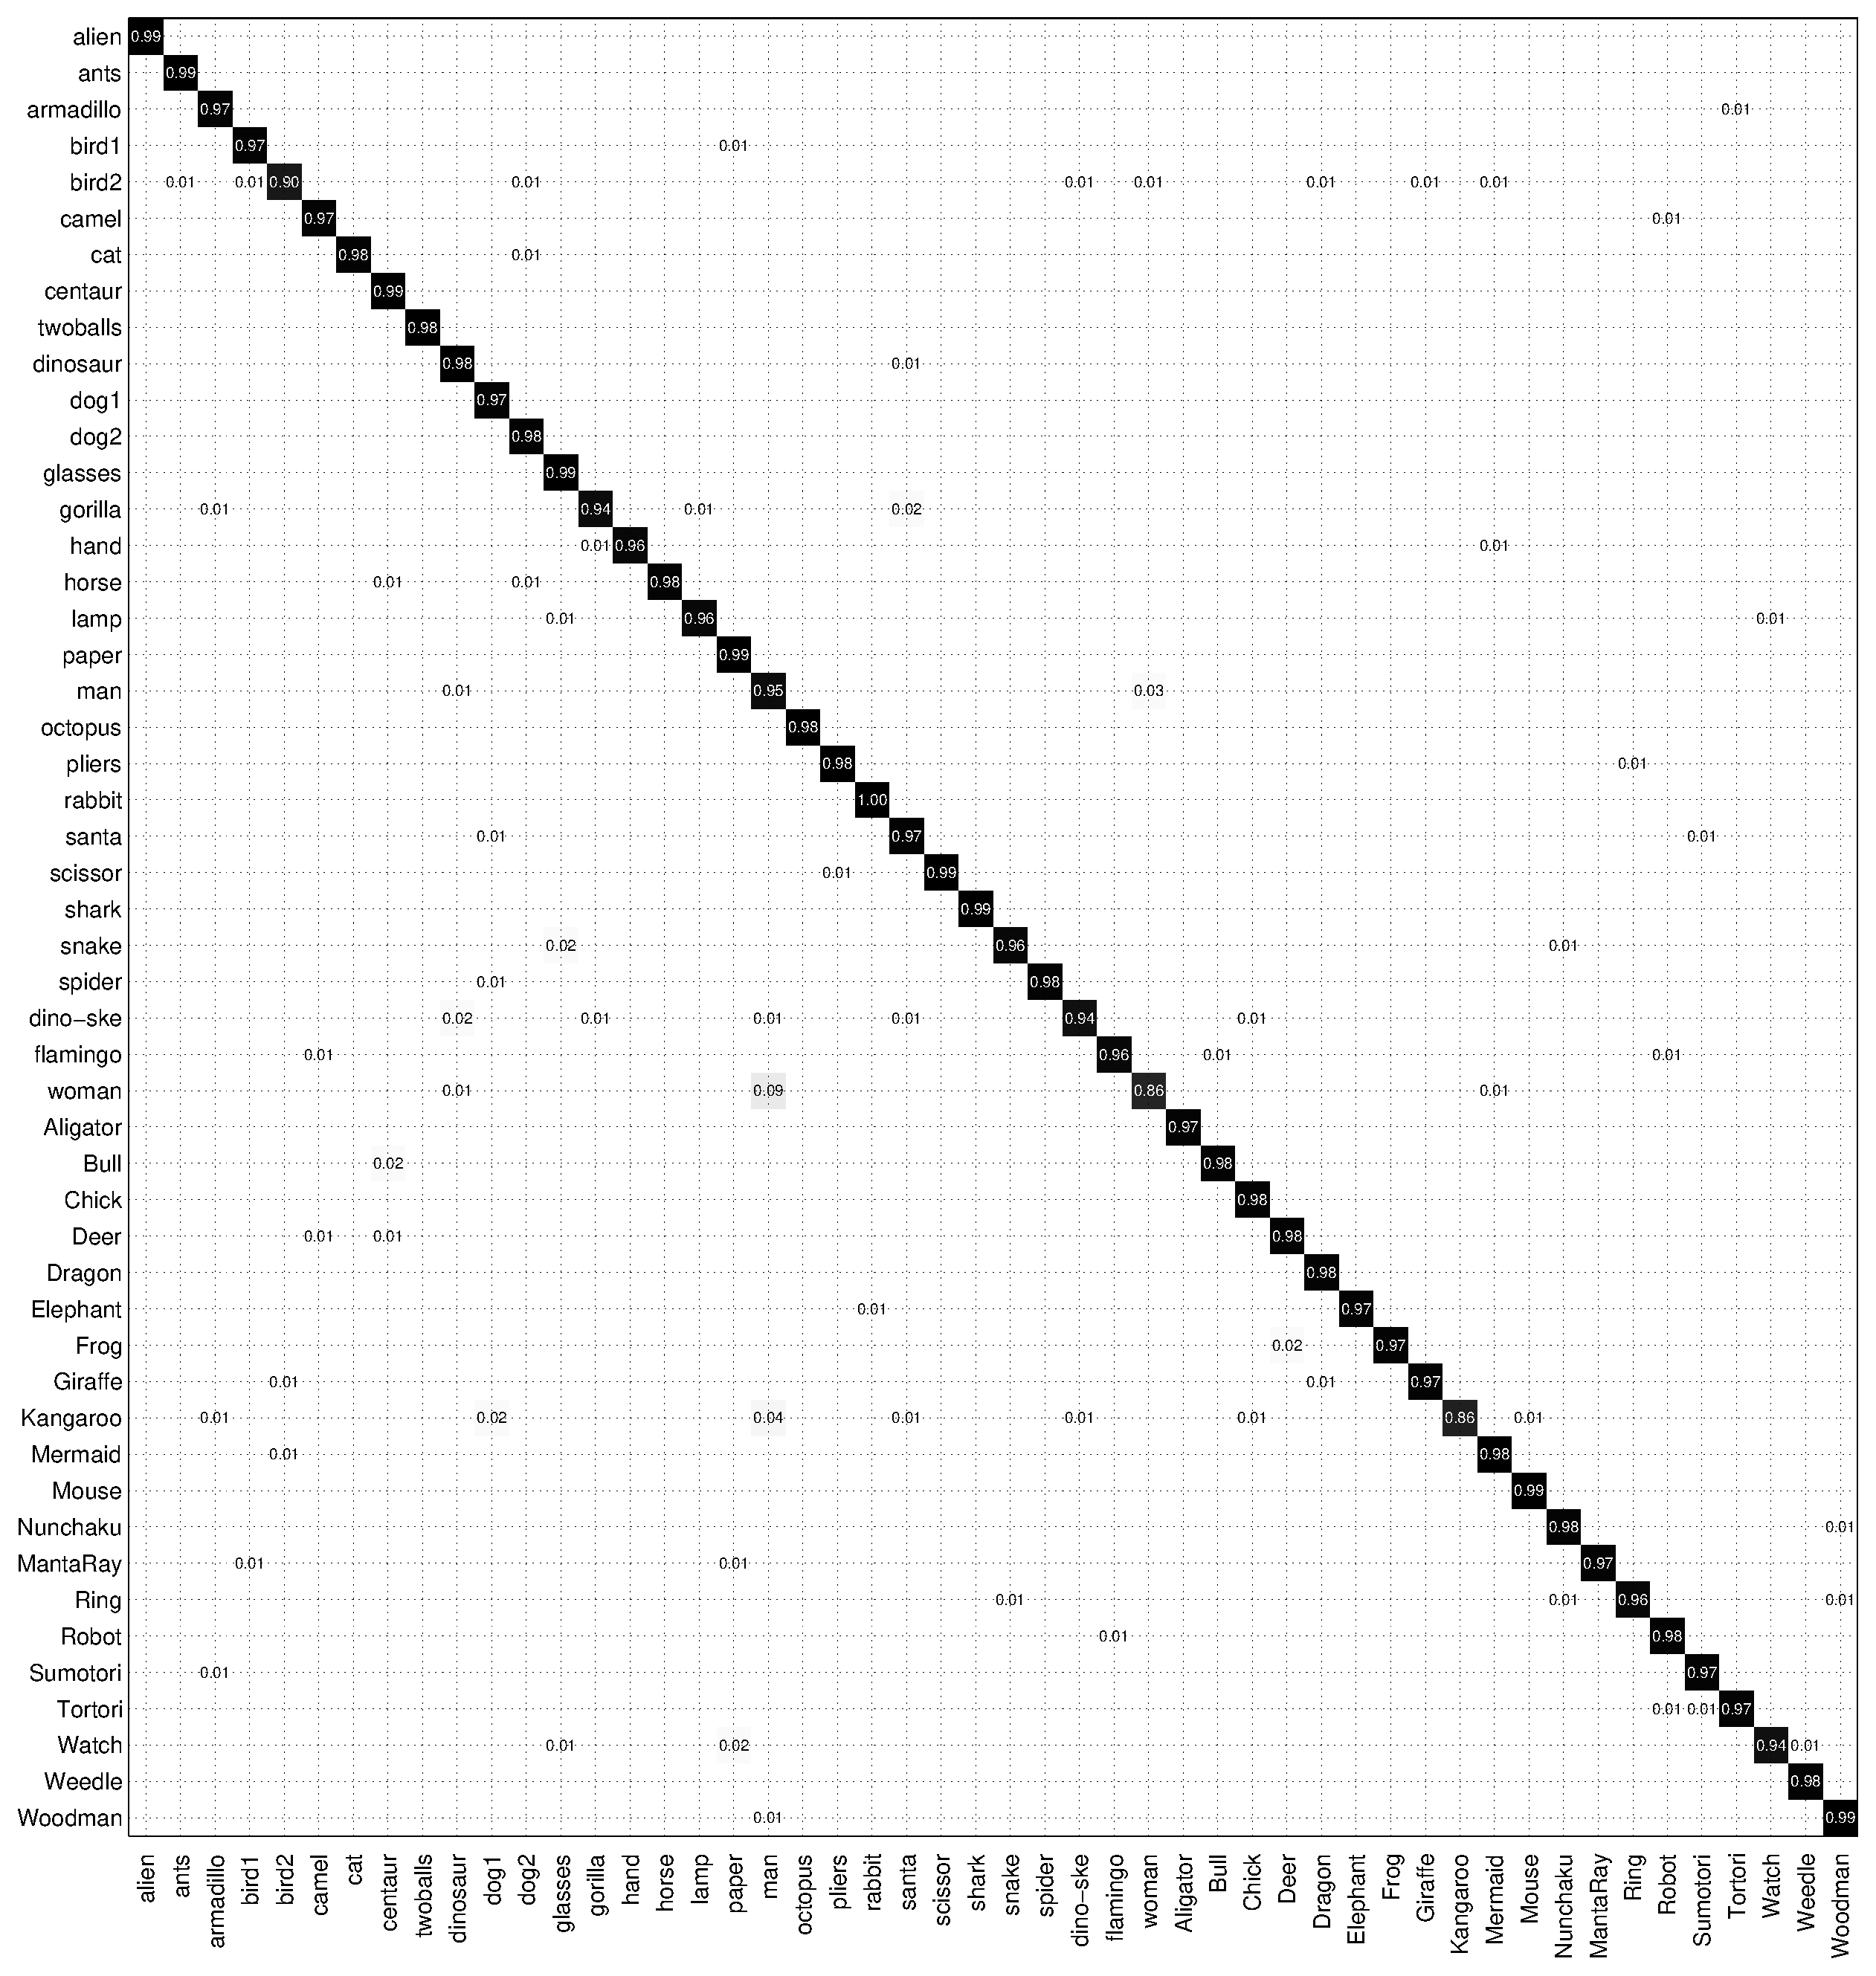
\includegraphics[width=0.45\linewidth]{figures/shrec2015_CM_3view.eps} 
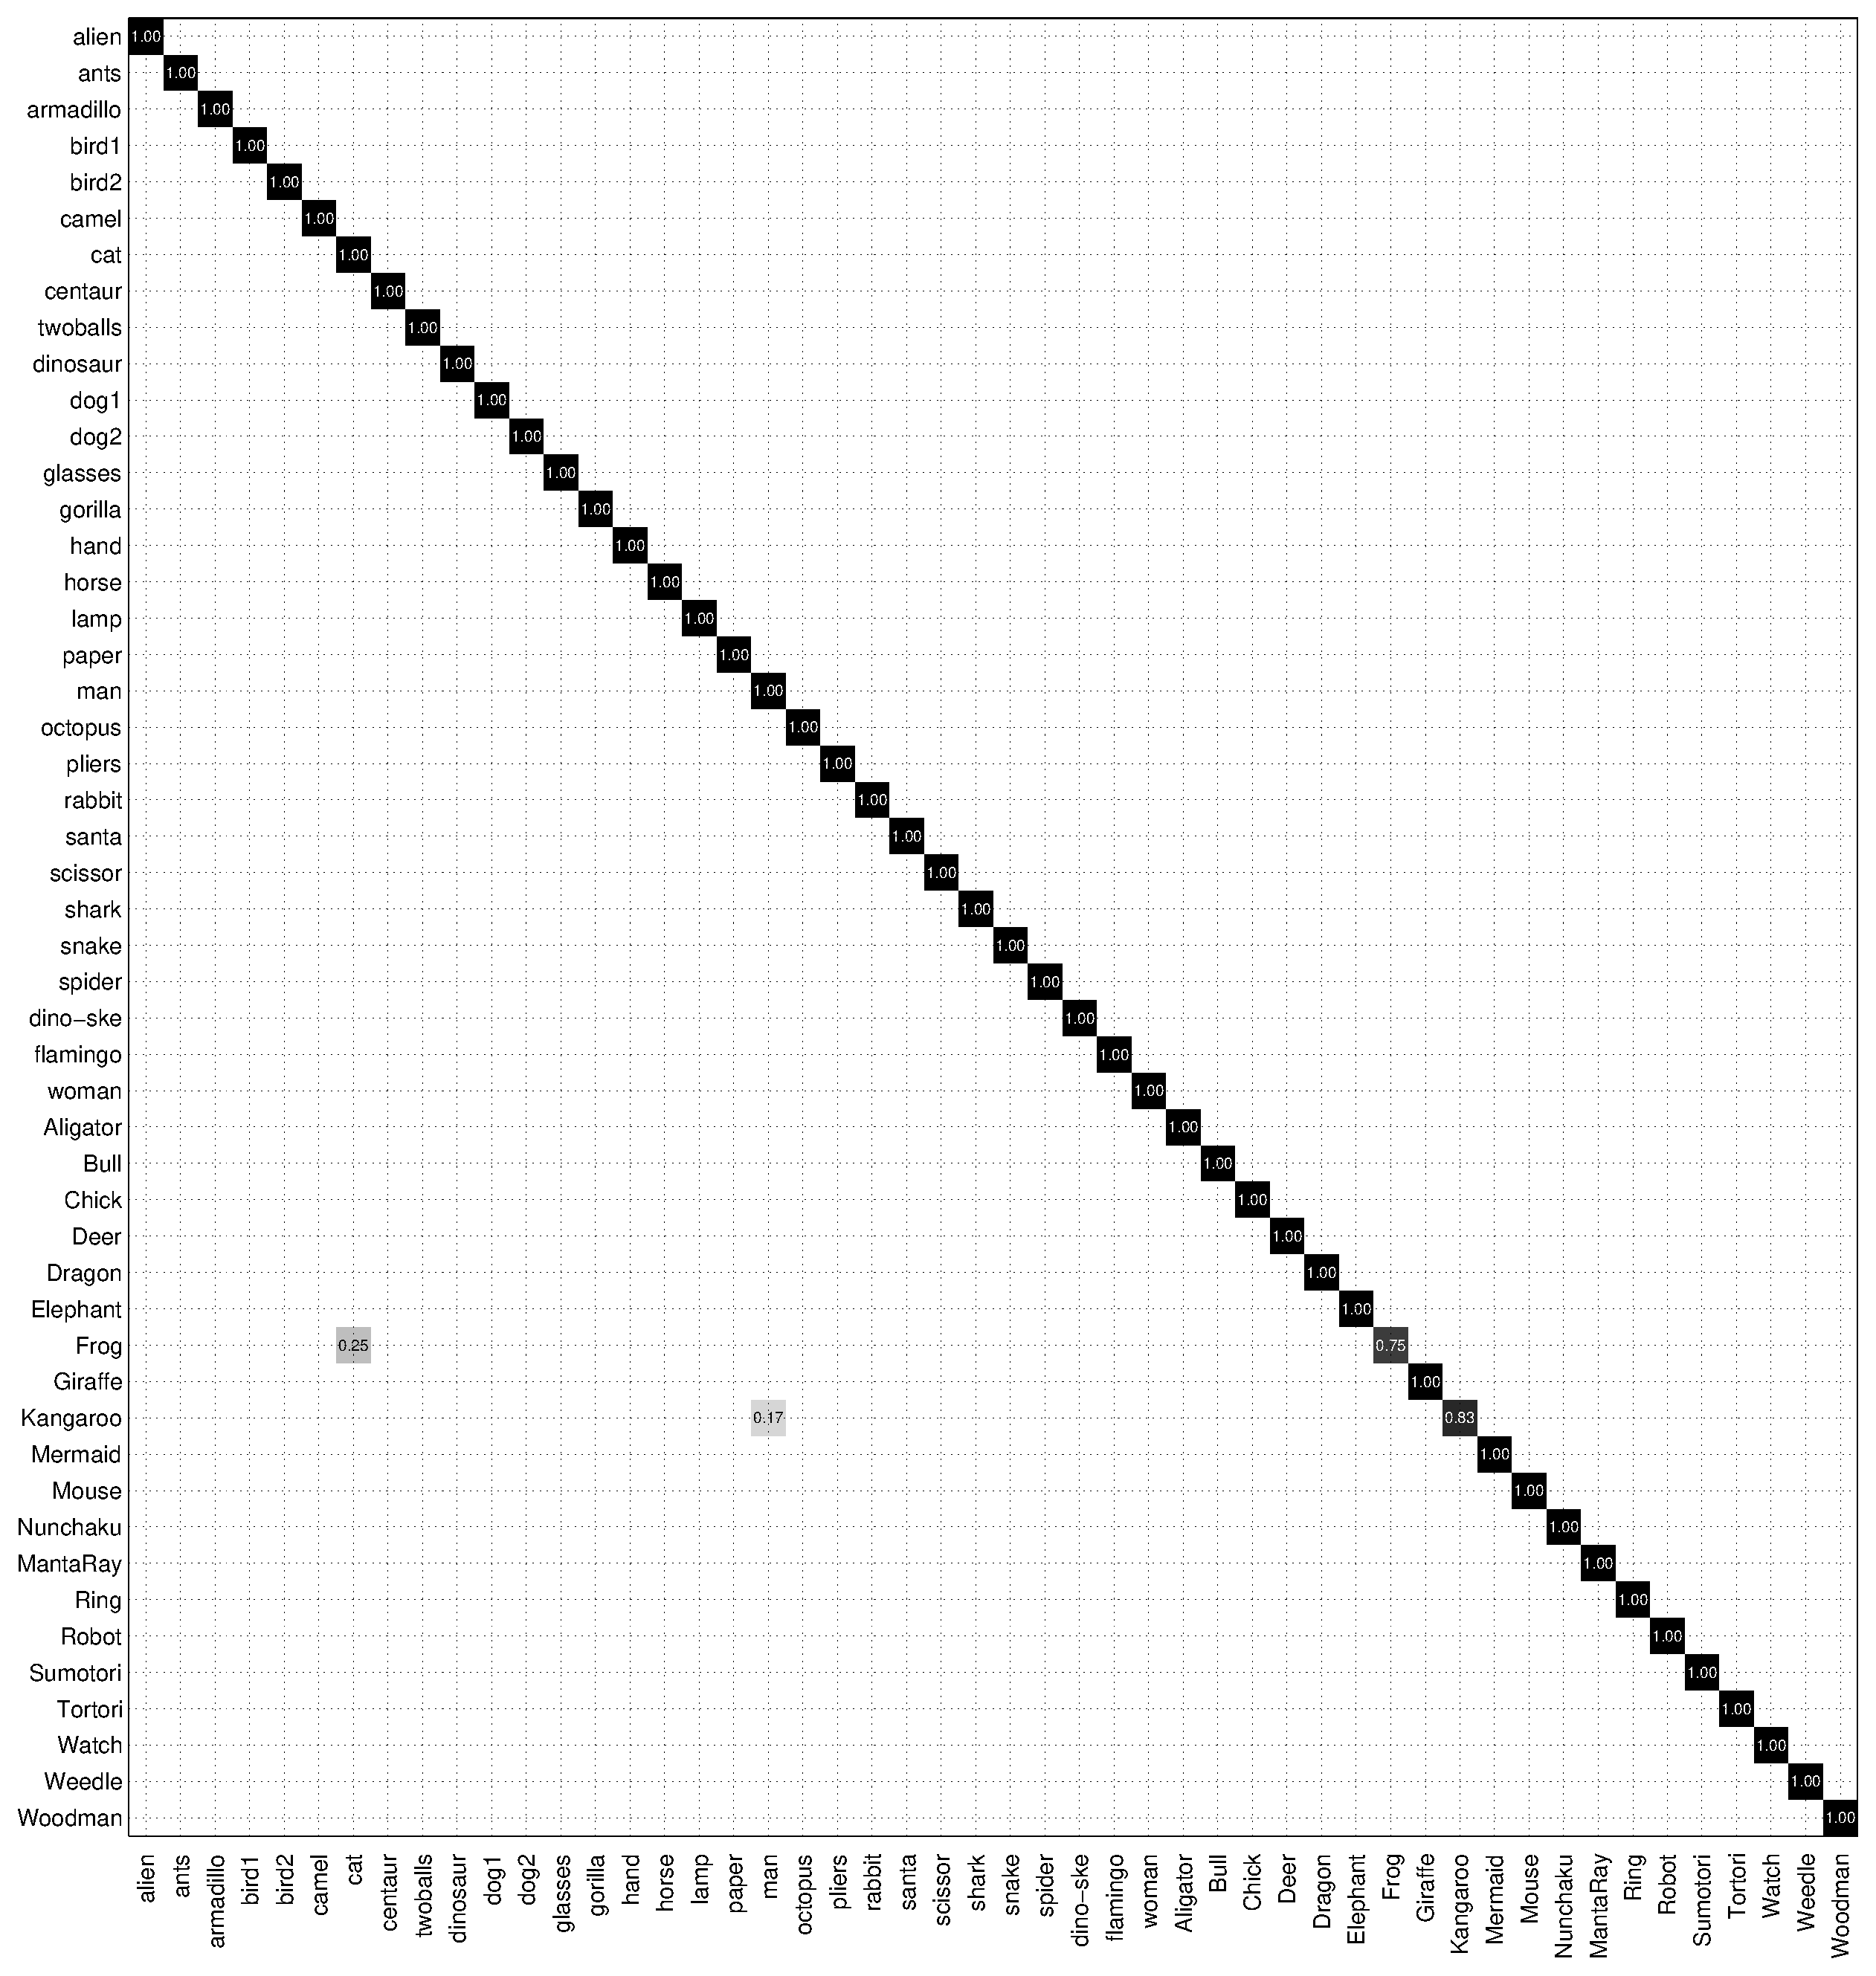
\includegraphics[width=0.45\linewidth]{figures/shrec2015_CM_200view.eps}
\end{center} 
\vspace{-4mm}
\caption{SHREC 2015的3个视图(左)和200个视图(右)的混淆矩阵} \label{fig_cm_shrec2015}
\end{figure*}


在机器学习领域,混淆矩阵是一种特定的表格布局,可以显示算法的性能。混淆矩阵包含有关分类系统完成的实际分类和预测分类的信息。为了进一步详细分析识别结果,使用所提出的方法在四个数据集上进行分类的混淆矩阵中 \ref{fig_cm_shrec2015}。实际上,每一行的总和是一个,因为它们是一个模型,但是,我们只画出了大于0.01的值,这使得一些行的总和不等于$ 1 $。从结果中,我们可以绘制得出的结论是该方法具有广阔的应用前景。横坐标表示实际分类,纵坐标表示预测分类。如图\ref{fig_cm_shrec2015}所示,SHREC 2015数据集混淆矩阵只有3个视图和200个视图。在左图中,虽然错误分类超过了右图,但分类准确性也被接受,因为分类错误的精度非常低。右图中,'猫'的25%被错误分类为'青蛙',同时17% “被误称为”袋鼠“。这种现象可能是由于猫和青蛙产生的一些相似的视图,而“袋鼠”和“人”也是相似的。但平均分类精度接近100%,说明该方法具有广阔的应用前景。
\begin{figure}[tbhp]
\begin{center}
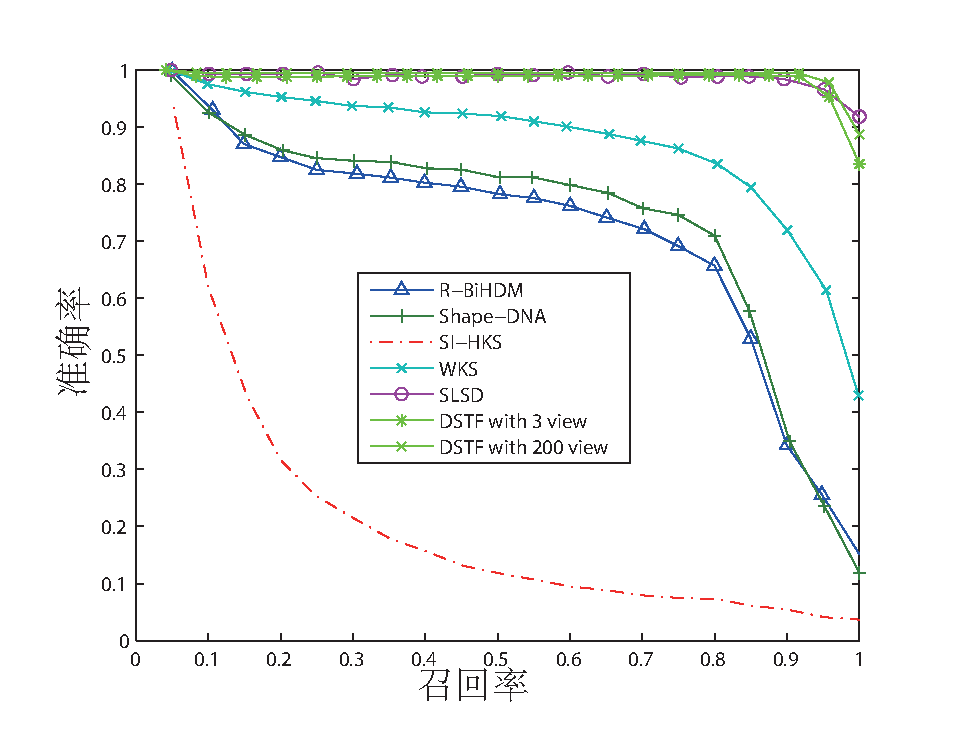
\includegraphics[width=1\linewidth]{figures/all_rp_cl_shrec2015.eps}
\end{center} 
\vspace{-4mm}
\caption{SHREC2015上3视图和200视图的一些最先进的方法和提出的方法的PR曲线。} \label{fig_rp_shrec2015}
\end{figure}




%table
\begin{table}[tbhp]
\caption{采用SHREC2015数据集测量方法对不同方法进行检索性能(\%)} \label{table_retrieval_shrec2015}
\begin{center}
\begin{tabular}{cccccc}  % {lccc} 
\hline  \hline
方法	    						&NN     &FT     &ST     &E      &DCG \\ 
\hline 
HAPT \cite{Giachetti2012Radial} 	&99.8	&96.6	&49.1	&81.5	 &99.2 \\
HKS-TS \cite{Lian2015SHREC}			&6.5	&6.4	&6.2	&7.4	 &39.1 \\
SGWS \cite{Li2013A}					&97.3	&76.0	&40.7   &66.0	 &91.9  \\
EDBCF \cite{Laga2013Geometry}		&97.8	&79.1 	&44.2	&70.8	 &94.3 \\
SLSD	\cite{Hamed2017Nonrigid}	&99.3	&98.0	&49.5	&82.4    &99.4	\\
DSTF 3-views   						&98.6  	&94.2  	&49.1  	&80.6  	 &99.1 \\ 
DSTF 200-views   					&99.5  	&94.9  	&49.4  &81.1  	 &99.6 \\ 
\hline  \hline      
\end{tabular}
\end{center} 
\end{table}

\subsection{检索实验}
对于检索任务,有6个标准评估指标用于评估推荐方法的性能。 它们是 precision-recall curve, nearest neighbor (NN), first tier (FT), second tier (ST), E-measure (E), 和 discounted cumulative gain (DCG),详细的定义可以在\cite{shilane2004princeton}中找到。等式\eqref{cal_cal_distance}被用来描述两个模型之间的相似性。


\textbf {SHREC2015检索实验}。 我们在SHREC2015数据集上进行了检索实验,以评估检索性能。我们的方法和一些现有技术的方法的回想精度曲线绘制在图\ref{fig_rp_shrec2015},其中包括S-HKS\cite {Bronstein2010Scale},WKS\cite{Aubry2011The}和浅层学习形状描述符(SLSD)\cite{Hamed2017Nonrigid}。从图中可以看出,推荐的方法总体上达到了最佳的检索结果。同时,该方法提高了类内相似度,降低了类间相似度。 结果,检索性能得到改善。

表\ref{table_retrieval_shrec2015}列出了我们的方法和一些最先进的方法进行的数值评估结果,包括面积投影变换(HAPT)的直方图\cite {Giachetti2012Radial},HKS-TS \cite {Lian2015SHREC}, SGWS\cite {Li2013A}和EDBCF\cite {Laga2013Geometry}。 从表 \ref {table_retrieval_shrec2015}中,我们可以清楚地看到所提出的方法对于检索是非常好的,这表明STF适合于稀缺的视觉信息获得良好的检索性能。 所提出的方法对于视觉信息稀缺的移动机器人三维识别任务是一种有效的方法。


\begin{figure}[tbhp]
\begin{center}
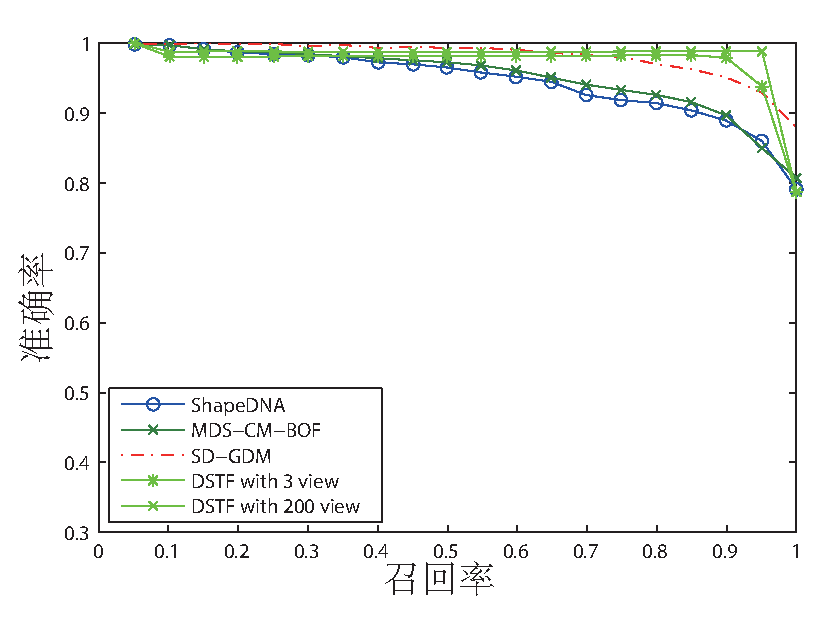
\includegraphics[width=1.0\linewidth]{figures/all_rp_cl_shrec2011.eps}
\end{center} 
\vspace{-4mm}
\caption{SHREC2011上的一些最先进的方法和提出的方法的PR曲线。} \label{fig_rp_shrec2011}
\end{figure}
%table
\begin{table}[tbhp]
\caption{采用SHREC2011数据集测量方法对不同方法进行检索性能(\%)} \label{table_retrieval_results_shrec2011}
\begin{center}
\begin{tabular}{cccccc}  % {lccc} 
\hline  \hline
方法      						&NN &FT &ST &E &DCG\\ 
\hline
Harris3DGeoMap \cite{Lian2011SHREC}	&56.2	&32.5	&23.3	&32.2	&65.4	\\
BOW-LSD \cite{Lavou2011Bag}				&95.5	&67.2 	&40.2	&57.9	&89.7 \\
ShapeDNA \cite{Reuter2006Laplace}		&99.2 	&91.5 	&47.9	&70.5	&97.8	\\
MeshSIFT \cite{Maes2010Feature}		&99.5	&88.4	&48.1	&70.8	&98.0	\\
DSTF	3-views								&97.7	&92.1	&48.7	&71.0	&98.6	\\
DSTF	200-views							&98.7	&93.5	&48.9	&71.4	&99.0	\\
\hline  \hline      % 
\end{tabular}
\end{center} 
\end{table}


\begin{figure}[tbhp]
\begin{center}
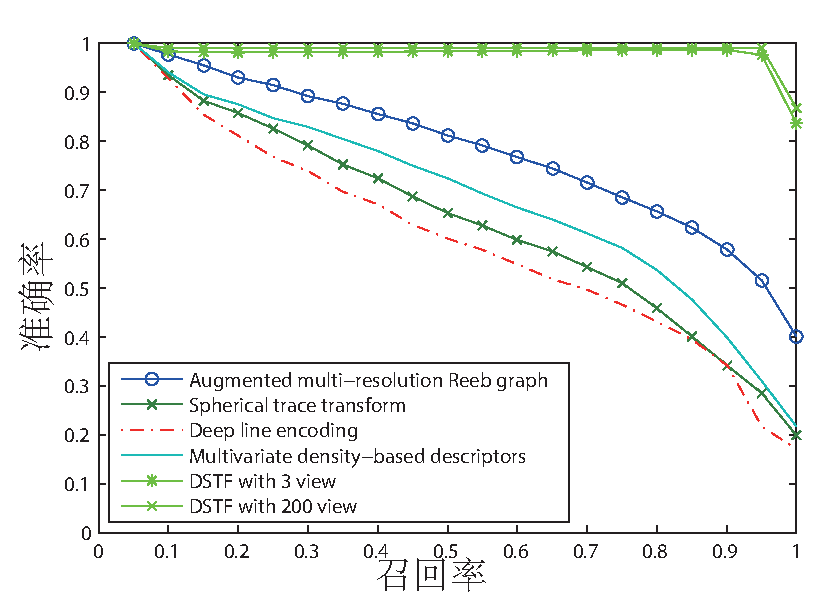
\includegraphics[width=1\linewidth]{figures/all_rp_cl_shrec2007.eps}
\end{center} 
\vspace{-4mm}
\caption{SHREC2007上的一些最先进的方法和提出的方法的PR曲线。} \label{fig_rp_shrec2007}
\end{figure}

%table
\begin{table}[tbhp]

\caption{采用SHREC2007数据集测量方法对不同方法进行检索性能(\%)} \label{table_retrieval_results_shrec2007}
\begin{center}
\begin{tabular}{cccccc}  % {lccc} 
\hline  \hline
方法	    &NN     &FT     &ST     &E      &DCG \\ 
\hline 
DSTF 3-views		&98.3	&92.2	&49.0	&71.4	&98.9	\\
DSTF	200-views	&99.0		&93.8	&49.2	&71.8	&99.3	\\
\hline  \hline      
\end{tabular}
\end{center} 
\end{table}



\begin{figure}[tbhp]
\begin{center}
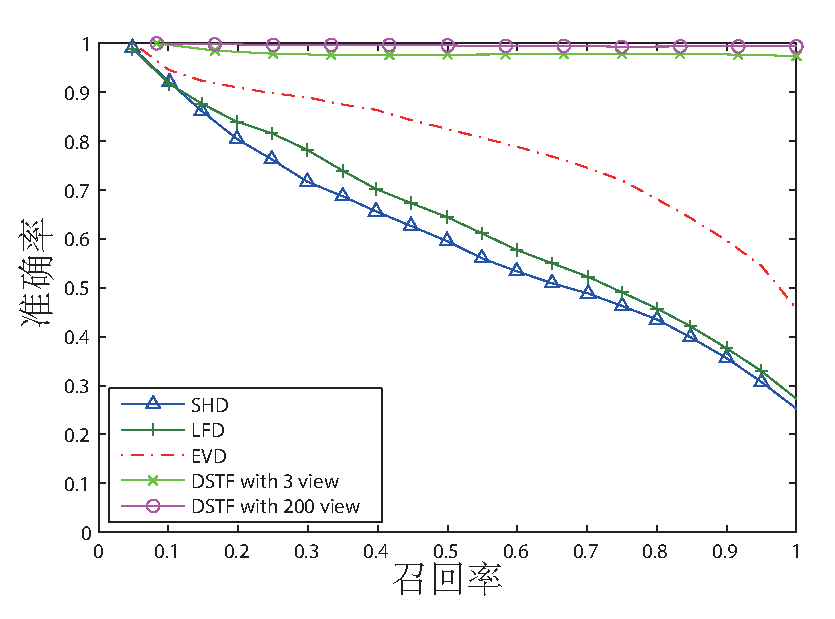
\includegraphics[width=1.0\linewidth]{figures/all_rp_cl_McGill.eps}
\end{center} 
\vspace{-4mm}
\caption{McGill上的一些最先进的方法和提出的方法的PR曲线.} \label{fig_rp_McGill}
\end{figure}

%table
\begin{table}[tbhp]

\caption{采用McGill数据集测量方法对不同方法进行检索性能(\%)}\label{table_retrieval_results_McGill}
\begin{center}
\begin{tabular}{cccccc}  % {lccc} 
\hline  \hline
方法                 &NN &FT &ST &E &DCG\\ 
\hline     
DSTF 3-views					&97.8 &92.9 &48.7 	&81.3		&98.7 \\
DSTF 200-views				&99.8 &	94.9 &49.6	&83.2		&99.7	\\
\hline  \hline      %
\end{tabular}
\end{center} 
\end{table}








\textbf{SHREC 2011, SHREC 2007和McGill检索实验。} 我们还对SHREC 2011,SHREC 2007和McGill数据集进行检索实验,以评估检索性能。我们的方法和一些最先进的方法,包括深度线编码(DLE)\cite {giorgi2007watertight},多元密度描述符(MDD)\cite {giorgi2007watertight},球形轨迹变换(STT )\cite {giorgi2007watertight},增强的多分辨率Reeb图(aMRG)\cite {giorgi2007watertight},ShapeDNA \cite {Reuter2006Laplace},MDS-CM-BOF\cite{lian2010non},SD-GDM \cite{Lian2011SHREC} 球面谐波描述子(SHD)\cite{Kazhdan2003Rotation},光场分布(LFD)\cite{chen2003visual}和EVD \cite {gal2006salient}绘制在图\ref {fig_rp_shrec2011}, \ref {fig_rp_shrec2007}和\ref {fig_rp_McGill}。与这些方法相比,我们的方法要好于其他方法。表\ref {table_retrieval_results_shrec2011},\ref {table_retrieval_results_shrec2007}和\ref {table_retrieval_results_McGill}列出数字评估。结果表明,提出的框架是对于视觉信息稀缺的三维形状进行识别良好效果。


\section{总结}
在本节中,我们提出了一个新的三维形状识别和检索框架,以解决移动机器人面临的信息缺乏的三维形状识别问题。首先,视觉描述符被提取为基于视图的CNNs特征。 然后将不同的视觉描述符作为LSTM的输入,以了解它们之间的顺序关系。 CNN模型就像人类的“视觉系统”一样,从单幅图像中学习视角的特征。 而且,LSTM模型与“记忆系统”类似,挖掘了不同视觉特征的内在时空关系。在分类和检索任务的标准基准上进行的实验已经证明,与最先进的方法相比,推荐的方法实现更好的性能。 实验结果表明,提出的表示方法具有较强的判别能力,能够抑制类内变异,增强类间相似性分离。与传统的计算机视觉形状分析方法不同,我们充分考虑了视觉特性和时空序列特性。 通过使用这种策略,可以对高度非线性的相关性视图模式进行全面建模。

\textbf{局限性。} 我们处理每个视图都是同等重要的,但是有些视图比其他观点重要得多。 最佳视图选择在时空建模中应该被考虑。有限数据集限制了神经网络的规模。 小规模的数据集不能完全训练一个更大的深度学习网络,影响进一步的应用。

\textbf{未来工作。} 首先,目前各视角的权重是相等的,不符合实际。 为了提高所提模型的适应性,应该增加图像权重,从而得到更好的性能。其次,进一步的应用需要更大的神经网络来完成更复杂精细的工作。 因此,有必要建立一个更大的三维形状数据集,以适应更大的深度学习网络。 



% 第五章
\chapter{总结与展望}

随着具有更强大功能的新型捕捉设备的不断演进,给三维形状分析领域带来了新的机遇,同时也带来了新的挑战。 深度学习彻底改变了很多二维计算视觉任务,有的甚至超越人类的表现,现在它也开始在3D领域进行扩展。尽管3D数据提供了更精确,更有区别力的表示,但其内在的复杂结构使得它们在深度架构中的应用是具有挑战性的。

\section{全文总结}

\subsection{基于多模态深度学习的三维形状识别与检索}
随着信息时代的到来,3D形状作为一种多媒体数据,已经广泛应用于计算机图形学和计算机视觉应用领域,如多媒体游戏,医学诊断,工业设计,信息检索等。所有这些应用程序都需要对3D模型进行有效的自动存储,识别和检索。因此,建立一个高效的形状搜索引擎是非常重要的,通过这个引擎,用户可以方便地获得三维模型,并进一步探索。而搜索引擎的核心需要有效的检索和分类技术来管理和重用三维形状。在过去的几十年中,对文本和图像的分析和检索进行了大量的努力,取得了很好的成果。然而,由于三维形状的特征与文本和图像有很大的不同,这些成功的识别和检索方法不能直接应用于三维模型,因此对三维形状的分析和理解仍然是一个长期的研究课题。近年来,对于三维形状识别,匹配和检索问题已经有许多解决方案。回顾这些解决方案的实现,我们发现它们与形状描述符直接相关,用于描述与其他形状或局部区域相区别的重要特征。许多早期的主要形状特征取决于人类设计或手工制作,从三维模型中捕捉一些特定的信息,如几何,拓扑和部分级结构。

三维形状由复杂的拓扑结构和明显的变化几何构成。因此,只有有限的信息可以用手工特征方法来提取。为了进一步提高3D形状描述符的性能,另一种方法是从复杂的3D数据中学习隐藏状态。自动特征学习方法的最近成功引起了计算机视觉和机器学习领域的广泛兴趣。这些方法可以从训练数据中自动学习特征,与根据人类先验知识设计特征的方式相比,这不仅可以减少工作量,而且还可以提取更高效的描述符。尤其是深度学习技术的快速发展,提高了特征表示能力,提高了识别任务的性能。直接采用深度学习技术来提取三维形状描述符似乎很困难,因为三维模型通常表示为与二维图像表示不同的二维流形。对于3D几何模型的编码没有一个标准的程序。为了解决这个问题,最常见的思想是将3D形状转换成图像表示,然后使用深度学习技术来处理这些图像。

然而,仅从视点方面分析3D数据对于3D形状理解来说仍然不够,因为在将3D形状转换为2D图像时,3D空间几何信息不可避免地丢失。 在现实世界中,人类通过各种各样但不可能相互独立的信息来理解对象。 例如,视频通常包括视觉和音频信号,与标题和标签相关的图像。 因此,对于3D形状,它包括从各个角度捕捉的多视图图像并形成固有属性。 由于描述相同对象的这些特征,它们具有一些高度非线性的关系。 然而,不同形式的这些特征具有不同的表现形式和结构。 三维物体的特征往往包括几何结构和拓扑关系的信息。 正因为如此,挖掘不同形态特征之间隐藏的非线性关系是一个挑战。

在第三章的工作中,我们提供了一个综合考虑三维形状的外在属性和内在特征的解决方案。 我们提出了一个新的方案来融合3D形状的不同形态数据到深度学习框架。 其核心思想是运用深度学习技术,结合利用三维模型本身的复杂拓扑关系和几何特性的基于几何的算法的优点,以及基于视觉的特征方法从不同视图中提取三维模型视觉特征的优点。 简而言之,分别采用卷积深度信任网络(CDBN)和卷积神经网络(CNN)分别从几何模态和基于视图的模态学习三维形状。 接下来,这两种模式与受限玻尔兹曼机(RBM)融合以获得更多的判别特征。 该计划包括以下三个主要部分:

\begin{enumerate}
\item \textbf{视觉特征学习}: 首先,每个3D形状由来自不同视图的一组2D图像表示。接下来,由于CNN在计算机视觉领域具有出色的视觉特征提取能力,所有这些投影都被用来训练CNN获取三维形状的视觉表示。
\item \textbf{几何特征学习}: 由于卷积运算具有旋转和平移不变的优点,并且将其集成到神经网络中实现了权重共享,由于减少了参数数量,CDBNs被用来学习几何特征。首先将三维形状转换为容易输入到CDBN模型的体积表示,然后用它来学习三维形状的几何表示。
\item \textbf{模态特征融合}: 上面提到的两种类型的特征代表了三维形状的不同方面信息。我们使用DBN来进一步探索它们的高级表示,这些表示被称为高级视觉描述符(HVD)和高级几何描述符(HGD)。然后利用RBM将两种模态高层特征相关联,挖掘其非线性信息,生成更强的代表性特征,即3D多模态特征(3D MMF)。
\end{enumerate}

这个框架的优点如下:
\begin{itemize}
\item 融合不同的形式来全面理解3D形状。
\item 在不同的特征提取程序中使用不同的深度学习技术充分利用各种深度学习方法从三维模型中提取不同的属性。
\item 与其他需要手动调整参数以获得最佳性能的机器学习方法不同,在整个学习过程中没有要调整的参数。 提出的方案是自动学习的。
\end{itemize}


\subsection{用有限信息进行三维形状识别的深度空时网络}
随着机器学习技术的发展,智能化是移动机器人与现实环境互动,有效导航的趋势。传统上,普通相机被用来获取图像,以帮助移动机器人探索周围的环境。毕竟,这种方式只是获取2D信息,与它们的3D模型相比,包含了更丰富的信息保存实物的表面和纹理。因此,3D模型在移动机器人的感知环境中起着至关重要的作用。目前,微软Kinect等多种RGB-D传感器被开发出来,以便捷有效的方式获取3D数据,进一步导致3D数据爆炸。快速发展需要一个强大的形状搜索引擎,有效地实现检索和分类任务,这是移动机器人智能系统的必要组成部分。

对于形状搜索引擎,在过去的几十年里,对于三维形状识别和检索已经有了很多的解决方案。实现了三维形状描述符来表征重要的全局或局部属性,并与其他形状或局部区域进行区分,说明形状特征提取是设计形状检索系统的重要工作。

回顾以前的作品,基于视觉的特征和基于几何的特征是在分类和检索任务中应用的两种典型形状描述符。视觉描述符通常通过从不同视图中收集2D投影来提取,以描述3D对象,并且对3D模型表示伪像(如孔和噪声)有效。灵感来源于人类通常从不同角度学习基于2D外观识别3D对象而不是获得3D形状的概念。特定的早期工作是光场描述符(LFD),它从几个不同的视点提取一个从几何和傅里叶描述符中提取一个几何和傅立叶描述符,这提供了一个基本思想,可以很容易地将复杂的三维形状转换成二维图像用某些创造性技术进一步获得特征。几何描述符通常是基于三维网格的位置和方向,或在顶点上定义的坐标系统,如形状直径函数(SDF),平均测地距离(AGD)等等。这些方法的核心思想是构建复杂三维网格的几何,拓扑和纹理的数学模型。然而,3D形状由数百个顶点和面组成,形成复杂的拓扑结构。更糟糕的是,3D模型表面存在一些空洞和噪声,这是实际应用中常见的情况。建立一个完美的数学模型来描述网格上的三维数据特征是很困难的。与基于几何的方法相比,基于视觉的方法不需要指定相对于任意定义的坐标系的描述符位置。因此,视觉特征具有表示用于3D模型分析的3D形状的优点。

一般而言,基于几何和视觉的特征属于手工描述符,这增加了特征设计者的工作量,降低了智能系统的水平。进一步降低智能代理在各种复杂环境下的自我调节能力。近年来,深度学习技术是机器学习方法中的一种技术,由于其强大的学习深度和判别性高层特征的能力,在计算机视觉领域做出了突出的贡献。在最新的研究中,使用深度学习技术分析三维模型数据有两种方法:间接和直接的方法。这种间接的方法是基于这样一种思想,即利用深度学习工具来处理由三维数据产生的各种类型的二维信息。通过逐步的特征提取,将原始三维数据的低级特征转换为二维数据格式的中间级特征,再将二维信息馈入深度学习体系结构,学习高层次判别特征。主要贡献是建立三维数据与深度学习工具之间的桥梁。一般来说,由于图像特征提取能力突出,常常使用卷积神经网络(CNN)来分析三维数据生成的视点图像。直接的方法是将原始3D数据直接送入深度学习架构。尽管如此,大部分的成绩来自间接的深度学习描述,直接的方法仍然远远不能令人满意。主要有以下两个原因:首先,间接方法是将三维数据转换为二维信息,这一步被认为是将原始三维网格重建为图像格式数据的过程,将其转化为深度神经网络。它利用了最近深度网络架构的图像特征提取的优势。其次,由于三维形状复杂的几何和拓扑结构,直接利用原始三维数据深度网络提取的新特征仍然不能满足。如三维立体体积和坐标,对方向,位置和变换都很敏感。因此,三维预处理的方法,深层结构的输入数据格式以及深层网络的设计架构都会影响形状描述符的提取。

目前,间接深层描述符达到了最先进的表现,这是由于充分利用了视点转换技术和深度学习技术的优点而产生的。但是这些特征仍然忽略了两个关键点:一是在实际应用环境中,移动机器人无法获得关于一个三维物体的全部视图,实现识别和检索任务。所以它要求智能代理能够高度准确地理解一个视图很少的3D对象。其次,大多数深层的描述符都是在忽略序列视图之间的内在联系的情况下学习的,这些关联信息丰富。例如,人类无法用单一的视角对三维物体进行准确的分类,而具有持久记忆的人类大脑有助于他们更自信地了解周围环境。长期短期记忆(LSTM)是一种神经网络,能够使用记忆机制对数据之间的时间或空间关系进行建模。与前馈神经网络不同,它构建了一个内部状态,允许在神经网络中循环的信号流,这是保持顺序信息的关键。许多作品表明,这种创造性的神经网络已经成功应用于语音识别领域。通过对上述两个问题的分析,提出了一个新的框架,利用更有价值的信息实现三维物体识别,指导智能代理的行为。该框架的基本原理是采用LSTM提取不同视图的非线性关系,在这之前CNN被用来学习从3D对象转换的视图的深度学习描述符。通过监督学习,优化CNN和LSTM的模型参数,将新输入数据的LSTM输出称为深时空特征(DSTF)。


这个框架的优点如下:首先,它不仅考虑了视觉特征,而且包含了时空的顺序关系。而且,在不同的识别程序中使用不同的深度学习技术,充分利用各种深度学习方法提取3D模型的高层次判别特征。第三,与其他需要手动调整参数以获得最佳性能的机器学习方法不同,在整个学习过程中没有要调整的参数。 提出的方案是自动学习的。

\subsection{总结}

本文从两个思路来解决三维形状的识别任务。第一种思路是多模态特征提取与融合方法。首先,通过CDBN和CNN分别提取几何描述符和视觉描述符作为基于几何的特征和基于视图的特征。 然后,采用两个DBN学习结构化的高层描述符。 此外,为了发现模式之间的深层相互关系,我们利用RBM来融合这些高级特征。第二种思路是为了解决解决移动机器人面临的信息缺乏的三维形状识别问题,从稀缺视角的角度出发,首先,视觉描述符被提取为基于视图的CNNs特征。 然后将不同的视觉描述符作为LSTM的输入,以了解它们之间的顺序关系。 CNN模型就像人类的“视觉系统”一样,从单幅图像中学习视角的特征。 而且,LSTM模型与“记忆系统”类似,挖掘了不同视觉特征的内在时空关系。这两种思路都取得了不错的效果,是一种积极的探索。

\section{展望}
目前,虽然取得了不错的结果,但是在该工作中还是有很多局限性,比如在生成几何描述符的过程中,网格尺寸越小,精度越高,但计算量呈指数增长。 因此,应该设计一个合适的方法来平衡这两个方面。在我们的框架下,为了学习三维形状的融合表示,我们将不同模式的高层特征连接起来。 然而,每个形态特征携带的信息并不完全相同。 因此,应寻求解决办法来表示不同形式的重要性。 此外,在所提出的方法中,深度学习的特征是全局性的,使得三维形状的局部信息或多或少地丢失。 因此,该方法难以应用于更复杂的任务,如分割,局部检索和对称检测。我们处理每个视图都是同等重要的,但是有些视图比其他观点重要得多。 最佳视图选择在时空建模中应该被考虑。有限数据集限制了神经网络的规模。 小规模的数据集不能完全训练一个更大的深度学习网络,影响进一步的应用。

因此,对于未来工作的展望如下,为了更好地描述三维形状,我们将探索将各种形式的全局特征和局部特征相结合的可能性。 其次,研究其他方法可以保留更多的结构信息进行特征学习。第三,研究可以直接处理图形数据的深度学习方法。目前各视角的权重是相等的,不符合实际。为了提高所提模型的适应性,应该增加图像权重,从而得到更好的性能。其次,进一步的应用需要更大的神经网络来完成更复杂精细的工作。 因此,有必要建立一个更大的三维形状数据集,以适应更大的深度学习网络。 




\backmatter
\bibliographystyle{nputhesis}
% \bibliographystyle{plain}  
\bibliography{ref}

% 附录
\backmatter
\Appendix
%This is appendix.

% 致谢
\Thanks
在此论文完成之际,两年多的研究生学习生活也即将结束,回首往事,成长道路上的点点滴滴在眼前掠过,感慨良多。在这里衷心地向曾经关心和帮助过我的人致以谢意。

向悉心培养与指导我的导师布树辉教授,致以最真挚的敬意和谢意!布老师指导学生总是春风化雨,润物无声。论文是在布老师的精心指导下完成的。在论文选题、理论、实验研究到撰写的整个过程中,处处渗透着导师无尽的心血。布老师丰富的实践经验、精益求精的科研作风与实事求是的学术态度以及对科学事业执着的追求精神将使我受益终身。对我影响最深的就是布老师在大年初三就投身科研的勤奋的钻研精神和他勤于思考问题善于创造性思维的习惯。他不仅授我知识、教我做人,还在思想、工作和生活等方面也予以无微不至的关怀。三年时间,布老师伴我成长,育我成才,我为教研室奉献青春深感荣幸。点点滴滴,深心铭感,浩瀚师恩,无以为报。谨向导师致以最诚挚的敬意和由衷的感谢!同时感谢刘贞报老师的关心和指导。

整个研究生学习期间,教研室的各位兄弟姐妹给予我很多的关心和帮助,让我感受到大家庭般的温暖。感谢李城梁、韩鹏程、程少光、王旭斌、赵勇、孙林杰、邵海东、阎蒙、何必、樊大森、李洋、黄金鑫、太敏、王雅南师兄师姐;感谢张臻伟,杨君,贾真,吕剑锋,于忠良,卜士洋,刘文萌等同级同学,感谢张咪、范帝楷、程城、冷鹏宇、马文科、王伟、李清、贺宇、童品模等师弟师妹,大家互相关心、互相帮助,给我留下很多美好开心的回忆,感谢你们一直以来的支持和鼓励,尤其是在我完成论文期间对我的帮助。

感谢我的家人和朋友,你们的默默鼓励和支持是我前进的最大动力。

最后,由衷的感谢参加论文评审和答辩的各位专家和学者。

%相关工作
\Work
% TODO 如何直接引用使参考文献的内容显示在这里

\begin{enumerate}
\item Bu S, Wang L, Han P, et al. 3D Shape Recognition and Retrieval based on Multi-modality Deep Learning[J]. Neurocomputing, 2017, 259.
\item 专利:一种基于多视角信息融合的机器人三维形状识别方法
\item 软件著作权:RTMapper在线实时快速地图构建与定位系统[简称RTMapper]V1.0
\end{enumerate}


% \statement
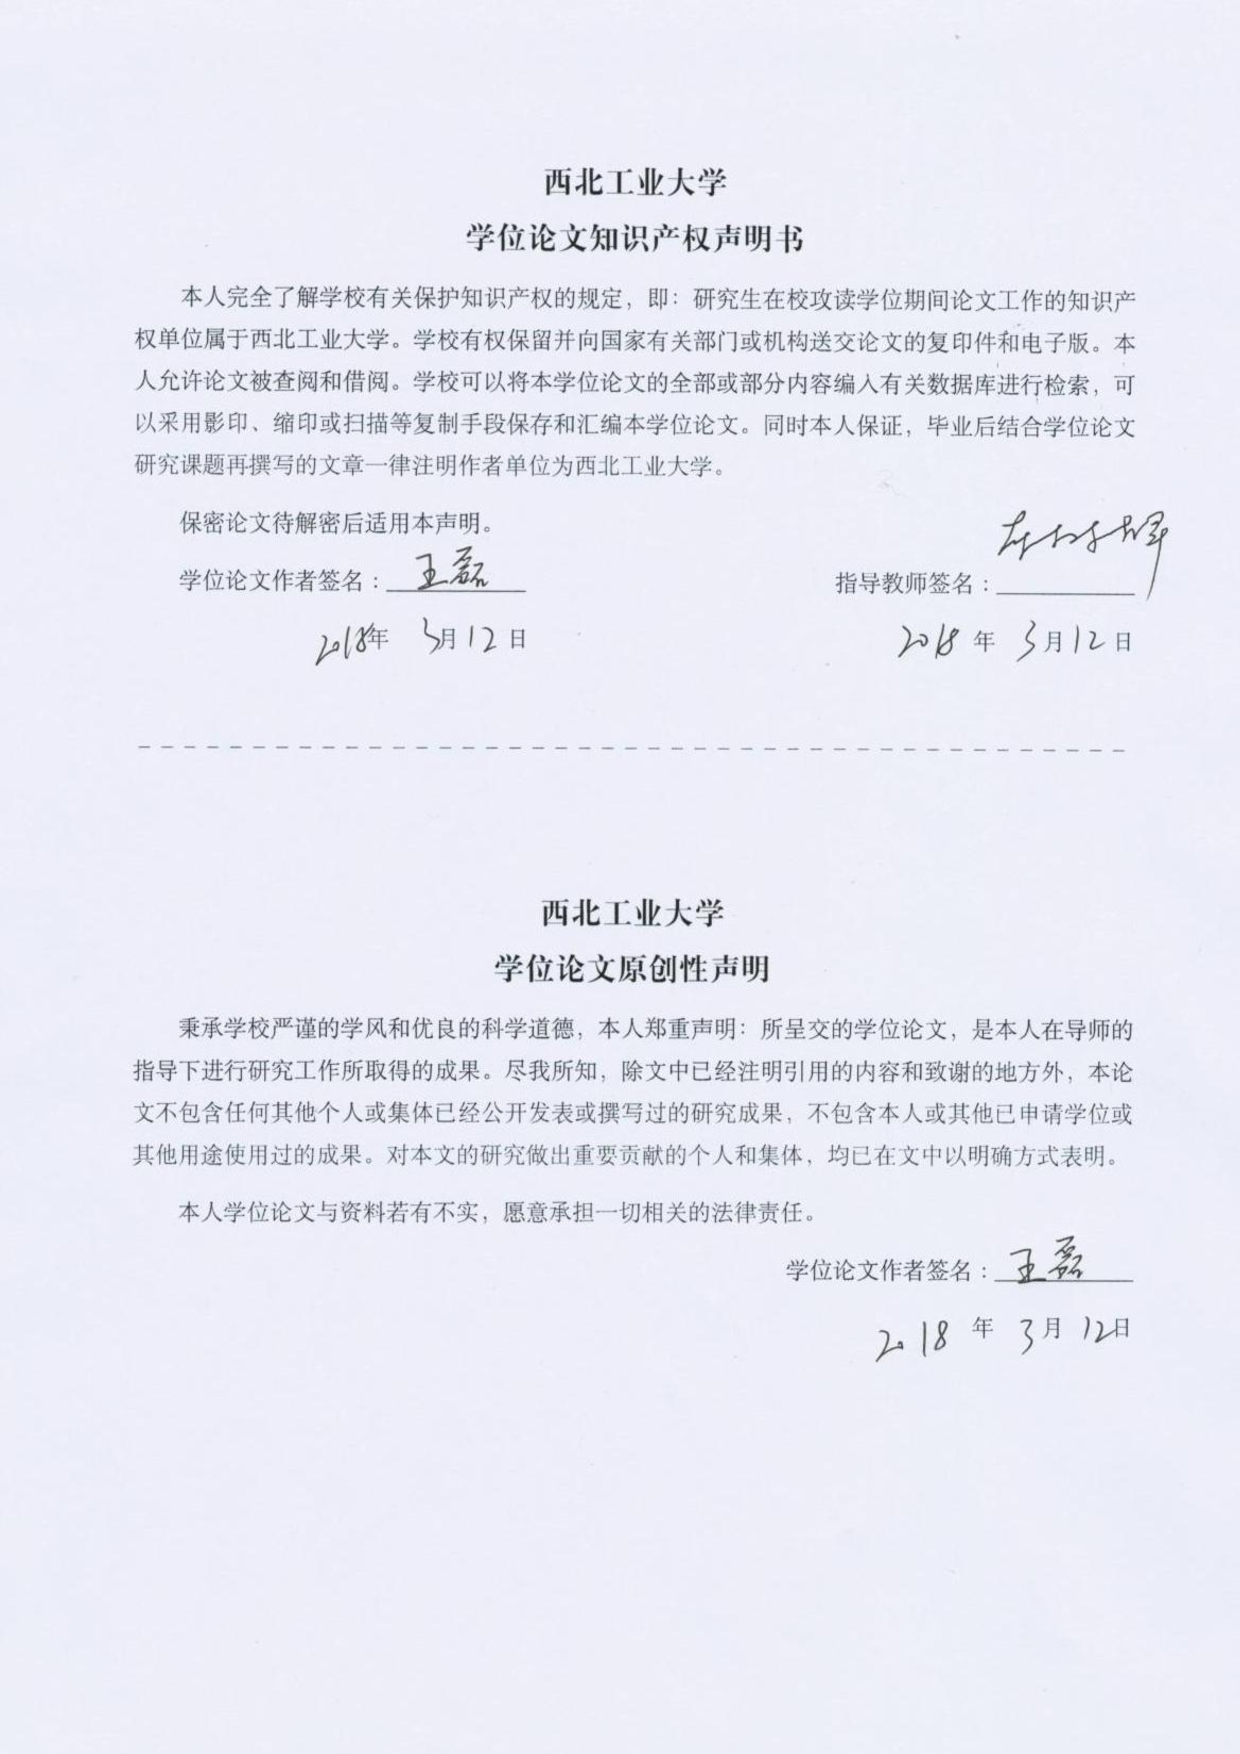
\includepdf{figures/签字.pdf} 
\newpage

\end{document}
